% Article in the format of the SBC Reviews journal (SBC Computing Reviews), English version.
% Translation of main.tex made by Claude Code (Claude Fable 5.2) on 24 November 2026 (D141), pending review by
% the author. The chapters are in capitulos-en/, one file per file of capitulos/; scripts/verificar_traducao.py
% compares labels, citations, identifiers and numbers between the two languages. Origin, version and limits of
% the adaptation are in TEMPLATE-SBC-REVIEWS.md. Compile with LuaLaTeX (make pdf-en).
\documentclass[english]{sbcreviews-2025}

% Language-dependent texts, used by sbc-comum.tex and by referencias.bib.
\newcommand{\SBCrotulopendente}{Pending}
\newcommand{\SBCorcidpendente}{ORCID pending}
\newcommand{\SBCemailpendente}{e-mail pending}
\newcommand{\versaoconsultada}[1]{Version consulted: #1}
\newcommand{\publicacaoantecipada}{Online-first publication, with no volume assigned.}
% Preâmbulo comum às duas versões do artigo no formato SBC Reviews: main.tex (português) e
% main-en.tex (inglês). Cada versão define antes os textos que dependem do idioma:
% \SBCrotulopendente, \SBCorcidpendente, \SBCemailpendente, \versaoconsultada e \publicacaoantecipada.
% A classe sbcreviews-2025.cls não é alterada; ver TEMPLATE-SBC-REVIEWS.md.
\usepackage[bottom]{footmisc}
\usepackage{afterpage}
\usepackage{url}
% O estilo apalike-sol.bst imprime o DOI como texto; o pacote permite o sublinhado de um DOI fora do modo matemático.
\usepackage[strings]{underscore}
\setcitestyle{square}

\definecolor{engtitle}{rgb}{0.5,0.5,0.5}
\definecolor{darkblue}{rgb}{0.0,0.0,0.0}
\hypersetup{colorlinks,breaklinks,
            linkcolor=darkblue,urlcolor=darkblue,
            anchorcolor=darkblue,citecolor=darkblue}

% ---------- Pendências visíveis ----------
\newcommand{\pendencia}[1]{\par\noindent\textcolor{red!65!black}{\textbf{\SBCrotulopendente:} #1}\par}
\newcommand{\aconfirmar}[1]{\textcolor{red!65!black}{#1}}

% ---------- Referências ----------
% Identificador e endereço das referências que só existem no arXiv (campo howpublished do .bib).
\newcommand{\soartigo}[1]{#1}

% ---------- Adaptação dos arquivos escritos para a classe IEEEtran ----------
% Os capítulos abrem os apêndices com \appendices, comando da IEEEtran.
\newcommand{\appendices}{\appendix}
% As tabelas foram dimensionadas para a classe IEEEtran (coluna de 252 pt e página de 516 pt); aqui a
% coluna tem 240 pt e a página, 498 pt. Sem alterar os arquivos dos capítulos, o espaço entre colunas
% diminui e a tabela que ainda passar da largura disponível é reduzida até caber (no máximo 5\%).
\newsavebox{\SBCcaixa}
\newcommand{\SBCtabelasajustadas}{%
  \let\SBCtabular\tabular \let\SBCendtabular\endtabular
  \renewenvironment{tabular}%
    {\begin{lrbox}{\SBCcaixa}\SBCtabular}%
    {\SBCendtabular\end{lrbox}%
     \ifdim\wd\SBCcaixa>\linewidth\resizebox{\linewidth}{!}{\usebox{\SBCcaixa}}\else\usebox{\SBCcaixa}\fi}}
\AtBeginEnvironment{table}{\setlength{\tabcolsep}{4.5pt}\SBCtabelasajustadas}
\AtBeginEnvironment{table*}{\SBCtabelasajustadas}

% ---------- Campos do cabeçalho da revista: marcadores do template, preenchidos pelos editores ----------
\jid{ROCS}
\jtitle{SBC Computing Reviews, 202X, XX:1}
\issn{2966-3938}
\doi{10.5753/rocs.202X.XXXXXX}
\copyrightstatement{This work is licensed under a Creative Commons Attribution 4.0 International License}
\jyear{202X}

% ---------- Título e autoria ----------
\newcommand{\titulotcc}{Revisão Rápida da Literatura: Engenharia de Prompt para Codificação e Implementação de Software}
% Título em inglês proposto por Claude Code em 24/11/2026; pendente de aprovação do autor (D141).
\newcommand{\titulotccen}{Prompt Engineering for Software Coding and Implementation: A Rapid Literature Review}
\newcommand{\nomeorientador}{Eduardo Magno Lages Figueiredo}
\newcommand{\nomecoorientador}{Pedro Saint Clair Garcia}

% Autoria: orientador como coautor por decisão do autor em 08/11/2026 (D88); coorientador informado
% em 21/11/2026 (D136), coautor por pedido do autor em 22/11/2026 (D138), com vínculo ao DCC/UFMG
% informado pelo autor (D139), não conferido em fonte institucional.
% ORCID e e-mail vêm de busca em fontes públicas feita em 24/11/2026 (D142) e estão A CONFIRMAR:
%  - Eduardo Figueiredo: ORCID no registro público do ORCID (vínculo UFMG, doutorado em Lancaster);
%    e-mail no perfil do DCC/UFMG (https://dcc.ufmg.br/professor/eduardo-figueiredo/).
%  - Pedro Garcia: ORCID de «Pedro Garcia» (UFMG), com obra assinada por «Pedro S. C. Garcia» em
%    coautoria com Eduardo Figueiredo (doi:10.5753/sbes.2024.3503). E-mail não localizado.
%  - Caio César de Freitas: ORCID não localizado; e-mail institucional não informado.
% O envelope marca o autor correspondente; a escolha do primeiro autor também está a confirmar.
\author[Freitas et al. 202X]{
\affil{\textbf{Caio César de Freitas}~\aconfirmar{[\SBCorcidpendente]}~\textcolor{blue}{\faEnvelope}~~[{Universidade Federal de Minas Gerais}~|~\aconfirmar{\textit{\SBCemailpendente}}~]}

\affil{\textbf{\nomeorientador}~\orcidlink{0000-0002-6004-2718}~[{Universidade Federal de Minas Gerais}~|\href{mailto:figueiredo@dcc.ufmg.br}{~{\textit{figueiredo@dcc.ufmg.br}}}~]}

\affil{\textbf{\nomecoorientador}~\orcidlink{0009-0005-7744-697X}~[{Universidade Federal de Minas Gerais}~|~\aconfirmar{\textit{\SBCemailpendente}}~]}
}


\category{Review}
\title[Prompt Engineering for Software Coding and Implementation]{\titulotccen}
\hypersetup{%
  pdftitle={\titulotccen},
  pdfauthor={Caio César de Freitas; \nomeorientador; \nomecoorientador},
  pdfsubject={Article in the SBC Reviews format -- Undergraduate final project -- Systems Engineering -- UFMG},
  pdfkeywords={prompt engineering, rapid literature review, code generation}
}

\begin{document}

\begin{frontmatter}

\maketitle

% Address from the footer of the DCC/UFMG website, consulted on 24 November 2026.
\begin{mail}
Departamento de Ciência da Computação, Universidade Federal de Minas Gerais, Av. Antônio Carlos, 6627, Prédio do ICEx, Pampulha, Belo Horizonte, MG, 31270-901, Brazil.
\end{mail}

\begin{abstract-en}
% Tradução do resumo (capitulos/00-resumo.tex) feita por Claude Code em 18/11/2026.
% Pendente de revisão do autor. Ao alterar o resumo, atualizar este arquivo.
Prompt engineering is one of the ways of using large language models in software development, and studies on the
subject vary widely in techniques, models, tasks and metrics. This work organizes the evidence on prompting
techniques applied to code generation, translation, refactoring and debugging, by means of a rapid review of the
literature, a taxonomy and a decision-support table. The search in arXiv, IEEE Xplore and the ACM Digital Library
returned 2,304 unique studies. Of these, 715 named the task in the title and were screened by two language
models, with checking by the author. At the full-text stage, the author checked the 419 studies read by the models
and included 332. The records of the 332 studies, with 805 comparisons and a quality assessment, were extracted by
AI; the author checked a sample of 67 studies, with corrections in 18 of 571 blocks, and checked against the
original papers the 120 empirical claims made in the text. Most of the evidence compares complete techniques with
baselines, without isolating the mechanism responsible. In the extracted comparisons, many favourable results
involve verifiable external information, such as tests, execution and repository context, and depend on more calls
to the model or on information from the reference solution. Reasoning instructions, self-critique without
execution, fixed examples and changes in wording had mixed results, especially with small models. Fewer than half
of the studies evaluate any risk mitigation. The main limitations are the requirement that the task appear in the
title, the exclusion of studies available only on arXiv and the extraction by AI, checked by the author only in a
sample.

\end{abstract-en}

\begin{keywords}
prompt engineering, code generation, rapid literature review, language models
\end{keywords}

\begin{dates}
% Dates filled in by the editors before publication.
\noindent{\sffamily\textbf{Received:}} DD Month YYYY~~~$\bullet$~~~
{\sffamily\textbf{Accepted:}} DD Month YYYY~~~$\bullet$~~~
{\sffamily\textbf{Published:}} DD Month YYYY
\end{dates}

\end{frontmatter}

% English translation of capitulos/01-introducao.tex, made by Claude Code (Claude Fable 5.2) on 24 November 2026.
% Pending review by the author. When the Portuguese file changes, update this one (scripts/verificar_traducao.py).
\section{Introduction}
Large language models (LLMs) have become part of software development tools. \citet{chen2021codex}, for
example, reported in 2021 the use of a production version of Codex in GitHub Copilot. As a result,
part of a programmer's work becomes writing instructions for the model, defining
context, examples and constraints. This practice is known as prompt engineering.

The literature on the subject is growing fast and uses techniques, models, tasks and metrics that differ
widely from one another. In the search carried out for this work, the same structure of terms retrieved 2,304
unique studies in three databases (Section~\ref{sec:busca}). This volume makes it hard to know what has already
been evaluated, under which conditions and with which limits. The motivation of this work is the expectation, which it
does not test, that an organized synthesis helps developers and researchers choose techniques
more judiciously.

The scope is restricted to pre-trained models used through prompts in four tasks: code generation,
translation, refactoring and debugging, including program repair. Training, fine-tuning
and model architecture are not covered, except when the study also evaluates prompting.
This work does not propose models and does not run experiments of its own to measure the effectiveness of
prompting techniques in the four tasks. LLMs are used and evaluated only in the operation of the review
(Section~\ref{sec:metodologia}), and those numbers do not answer the research questions.

\subsection{Objectives}
The objective is to organize evidence on prompt engineering techniques applied to code generation,
translation, refactoring and debugging, by means of a literature review and a
taxonomy to support developers. The specific objectives are:
\begin{itemize}
  \item to identify which prompting techniques are evaluated and what evidence of effectiveness is
  presented, under which models, tasks, metrics and conditions;
  \item to identify the technical risks reported and the mitigation strategies proposed or evaluated;
  \item to relate techniques, tasks and conditions in a taxonomy and in a decision-support table,
  examined in eight scenarios for clarity, grounding in the sources and concrete guidance.
\end{itemize}
This examination does not measure the effectiveness of the techniques or the productivity of those who use them.

\subsection{Organization of the paper}
Section~\ref{sec:fundamentacao} presents the concepts and the related work.
Section~\ref{sec:metodologia} describes the protocol, what was carried out and what is left for the final version. The following sections bring together the results, the discussion, with the
application that makes the decision-support table available for consultation (Section~\ref{sec:aplicacao}), and the conclusion.

% English translation of capitulos/02-fundamentacao.tex, made by Claude Code (Claude Fable 5.2) on 24 November 2026.
% Pending review by the author. When the Portuguese file changes, update this one (scripts/verificar_traducao.py).
\section{Background and related work}\label{sec:fundamentacao}
\subsection{Language models}
Current LLMs derive, to a large extent, from the Transformer architecture, based on attention
mechanisms~\citep{vaswani2017attention}. These models are pre-trained on large volumes of text and
directly model the probability of text sequences~\citep{liu2021pretrain}. They can therefore
be used in new tasks without changing the parameters, only by changing the input~\citep{sahoo2024survey}.
It is this possibility that separates the focus of this work from approaches based on training or fine-tuning.

\subsection{Prompt engineering}
A prompt is the instruction given to the model to enforce rules, automate processes and obtain certain
qualities in the output~\citep{white2023patterns}. Prompt engineering is the practice of designing these
inputs to obtain the desired behaviour from an already trained model~\citep{sahoo2024survey}.
\citet{white2023patterns} treat prompts as a form of programming and catalogue
reusable patterns, by analogy with software patterns.

\subsection{Prompting techniques}
The techniques below illustrate the kind of object the review intends to classify. The list is not
exhaustive, its presentation here does not indicate which one works best, and the mention does not decide the
eligibility of any family of studies.
\begin{itemize}
  \item \textit{Zero-shot}: only a natural-language instruction, without
  demonstrations~\citep{brown2020fewshot}.
  \item \textit{Few-shot}: the prompt includes a few demonstrations of the task.
  \citet{brown2020fewshot} evaluate this condition, alongside \textit{one-shot} and \textit{zero-shot},
  as ways of measuring in-context learning, so the two terms are not perfect synonyms.
  \item \textit{Chain-of-thought}: in the formulation of \citet{wei2022cot}, the demonstrations
  carry a series of intermediate reasoning steps. Variants without demonstrations will only be
  described if they appear in the corpus.
  \item ReAct: the model interleaves reasoning traces and actions, which allows it to consult external sources or
  environments~\citep{yao2023react}.
  \item \textit{Self-planning}: the model first plans the solution and then writes the code,
  from the plan~\citep{jiang2025selfplanningv5}.
  \item \textit{Self-debugging}: demonstrations teach the model to debug its own program,
  examining execution results and explaining the code~\citep{chen2023selfdebug}.
\end{itemize}
These items are not of the same kind: some describe a way of building the prompt, and others, a
sequence of interaction with the model.
For this reason, the synthesis uses two units. The technique, with the name given by the authors, is the unit of the comparisons.
The mechanism is the unit of the classification: each technique receives one or more labels from a closed dictionary of eleven
mechanisms, which are instruction, context, constraints, examples, decomposition, reasoning, feedback,
sampling, multi-agent, prompt optimization and other. Thus, an interaction sequence such as
\textit{self-debugging} appears as a combination of mechanisms, for example feedback, reasoning and
examples, and not as a category of its own. The classification is multi-label and distinguishes the mechanisms of the complete
package from those the technique adds to the base prompt.

\subsection{Tasks and forms of evaluation}
In this work, generation is the production of code from a description, specification or example.
Translation is the conversion of code between languages or platforms, including migration and transpilation.
Refactoring is the improvement of the structure of the code without a change in behaviour. Debugging and repair
consist of locating and fixing defects. Tests are included when they support these tasks. These
definitions delimit the scope of the review, but do not settle every borderline case:
Section~\ref{sec:metodologia} shows the calibration carried out and the cases still open.

Evaluation usually relies on benchmarks. HumanEval measures the functional correctness of
programs synthesized from docstrings~\citep{chen2021codex}. SWE-bench uses
real GitHub problems, in which the model has to edit a code base to resolve an
issue~\citep{jimenez2024swebench}. Results on these sets do not, by themselves, demonstrate
gains in productivity, security or cost. \citet{sallou2024breaking} discuss
threats to validity in the use of LLMs in software engineering, and part of them guides the quality
assessment planned in this work.

\subsection{Related work}
% AFIRMACAO: A119
\citet{hou2024slr} reviewed 395 studies on LLMs in software engineering, from January 2017 to
January 2024. On prompting, they describe the techniques and count their frequency: \textit{few-shot} in 88 studies,
\textit{zero-shot} in 79 and CoT in 18.
% AFIRMACAO: A120
\citet{fan2023survey} survey the area, rather than conduct a systematic review, and point to hybrid
techniques, which combine traditional software engineering and LLMs, as central to reliable results.
Both cover many software engineering activities, and not only prompting.
% AFIRMACAO: A121
In the opposite direction, \citet{sahoo2024survey} organize 41 prompting techniques by application area,
among them code-specific techniques such as \textit{Program of Thoughts}, SCoT and \textit{Chain of Code}, and
\citet{liu2021pretrain} systematize the prompting paradigm in natural language processing, without
restricting themselves to code tasks.

The search of this work also found closely related secondary studies, recorded as supporting material.
% AFIRMACAO: A122
\citet{yang2025aprsurvey} (S820) classify 66 LLM-based repair systems into fine-tuning,
prompting, procedures and agents and record, for the main result of each system, the benchmark, the
metric, the model and the assumption about fault localization.
% AFIRMACAO: A123
\citet{masthanali2026energy} (S1246) gather 18 studies on the energy efficiency of code
generated by LLMs and conclude that no prompting strategy improves it consistently across configurations.

This work crosses the two perspectives: prompting techniques in the four tasks, with extraction of the type of
counterfactual, the direction of each comparison, the evaluation conditions, the risks and the mitigations. The full
texts of these reviews were read, in the arXiv versions indicated in the references, for the comparison in Section~\ref{sec:comparacao}. Since the
search was not designed to locate reviews, no claim is made that this combination is new.

% English translation of capitulos/03-metodologia.tex, made by Claude Code (Claude Fable 5.2) on 24 November 2026.
% Pending review by the author. When the Portuguese file changes, update this one (scripts/verificar_traducao.py).
\section{Methodology}\label{sec:metodologia}
This section describes what was carried out up to 17 November 2026 and indicates what is left for the final version. The verb
tenses follow this distinction. The word ``pilot'' has three uses in the project records, which receive
distinct names here: the six reference studies of the initial analysis, the two screening
calibration samples and the full-text measurement.

\subsection{Type of study}
This work is a declared rapid review~\citep{cartaxo2020rapid}, reported according to PRISMA
2020~\citep{page2021prisma} where applicable. The original protocol defined a systematic literature
review according to \citet{kitchenham2015ebse}, complemented by
snowballing~\citep{wohlin2014snowballing}, and provided for a fallback to a rapid review if the former
proved unfeasible. The author adopted this fallback on 3 November 2026, before the batch screening, based on the effort
projection of Section~\ref{sec:calibracao} and with the agreement of the advisor.

Cartaxo et al. allow steps to be omitted or simplified, provided that the concessions are stated in the protocol and the
report warns about the limitations. The concessions adopted here are choices of this project, and not part of the
definition of a rapid review: requiring the task terms in the title, without broad snowballing, and reading
the studies from the text extracted from the PDFs. Since 8 November 2026, the version for the examining committee also leaves out the studies
that are only on arXiv, with no indication of peer review (Section~\ref{sec:textocompleto}). The execution is largely done by AI, with checking by the
author at defined points, and every inclusion is confirmed by the author.

\subsection{Research questions and criteria}
The research questions are: RQ1, which prompting techniques are evaluated and what evidence of
effectiveness is presented, under which models, tasks, metrics and conditions; RQ2, which technical
risks are identified and which mitigation strategies are proposed or evaluated; and RQ3, how to
relate techniques, tasks and conditions in a useful taxonomy.

The selection criteria are in Table~\ref{tab:criterios}. The protocol used only open-access texts. On 5 November 2026, after the title and abstract screening,
the author started to accept also texts obtained through the CAPES journals portal (Portal de Periódicos da CAPES), with UFMG access,
to reduce availability bias. The change is reported as a deviation; the remaining bias is a threat to validity.

The application of I2 at the full-text stage was defined on 3 November 2026, after the measurement of
Section~\ref{sec:calibracao}, and not from the beginning of the protocol. The measurement brought up cases that the draft
of the prompt (tc-v1) did not resolve: an observational study that analyses prompts without measuring their effectiveness
(S2261), a workflow that uses prompting techniques without isolating their effect (S306) and a decoding
strategy with no prompting technique evaluated (S2128), for which the author used X3, and the models, X4.
Under the rule decided, recorded in version tc-v2, the study must report a code result obtained by
prompting, with the prompt strategy described, without requiring a prompting comparator. Code as an
intermediate step is eligible if it is evaluated. An observational study that only describes the use, with no result
about the prompts, goes to the author as a doubt. An evaluated intervention that is not prompting is excluded as X4,
which broadens this code at the full-text stage; at the title and abstract stage, tr-v2 keeps the previous wording, with which
it was calibrated. The change is reported as a deviation from the protocol.

With tc-v2, the two models reread in new contexts, from the extracted text, S2261, S306, S2128 and S427,
the latter included to check whether the broadening of X4 would rule out a study that compares prompting with fine-tuning.
The two answered doubt, include, exclude by X4 and include, respectively. Since the rule was written
with these cases known, the agreement shows that it is applicable to them, but does not validate it in other studies.

\begin{table}[!htb]
\caption{Selection criteria}\label{tab:criterios}
\centering\footnotesize
\begin{tabular}{@{}lp{0.82\columnwidth}@{}}
\hline
I1 & Primary study.\\
I2 & Applies prompting of a pre-trained model to generation, translation, refactoring or debugging/repair; tests are included when they support these tasks.\\
I3 & Empirical evaluation or sufficiently described case study.\\
I4 & First public version between 1 January 2021 and 7 September 2026.\\
I5 & Text in Portuguese or English.\\
I6 & Full text in open or institutional access (CAPES/UFMG).\\
\hline
X1 & Duplicate or overlapping version of a study already recorded.\\
X2 & No technical detail to identify technique, task and evaluation.\\
X3 & Task out of scope (e.g., only summarization, code review or questions about code).\\
X4 & Centred only on training, fine-tuning or architecture; at the full-text stage, also another evaluated intervention that is not prompting.\\
X5 & Secondary study, position paper or tutorial.\\
X6 & Full text with neither open nor institutional access.\\
X7 & Outside the period or the language.\\
\hline
\end{tabular}
\end{table}

\subsection{Search and records}\label{sec:busca}
The search was run on 29 October 2026, by AI, and checked by the author. The same conceptual structure was
applied to title and abstract in arXiv, IEEE Xplore and the ACM Digital Library, combining three blocks:
prompting terms, terms for the four tasks and language-model terms. The syntax and the
filters were adapted to each database (Appendix~\ref{ap:busca}). Table~\ref{tab:busca} summarizes the collection.

\begin{table}[!htb]
\caption{Records exported per database (search of 29 October 2026)}\label{tab:busca}
\centering\footnotesize
\begin{tabular}{@{}llr@{}}
\hline
Database & Collection method & Records\\
\hline
arXiv & Official API, filter by day & 1,597\\
IEEE Xplore & RIS export, filter by year & 665\\
ACM DL & Result pages, filter by month & 482\\
\hline
\multicolumn{2}{@{}l}{Total} & 2,744\\
\multicolumn{2}{@{}l}{Redundant records grouped} & 440\\
\multicolumn{2}{@{}l}{Unique studies} & 2,304\\
\hline
\end{tabular}
\end{table}

IEEE Xplore displayed 671 results; the 665 exported do not include six courses, which had no export
option. The ACM collection used the result pages because the free edition does not offer
export, and the additional complete pass of 29 October was not preserved. On 1 November 2026, the collection was
repeated and preserved, with a different ordering: the 482 DOIs matched, and the check revealed three
titles truncated by the extraction, corrected in a traceable way. The match shows the same
set on the two dates, but does not guarantee the stability of the database index.

Deduplication used DOI, arXiv identifier and normalized title, and grouped the 2,744 records into
2,304 studies, without deleting the original records. Four of these studies belong to the reference
set~\citep{zhang2011identifying}, formed by six studies from the initial analysis: S1, on
\textit{self-planning}~\citep{jiang2025selfplanningv5}; S2, on
\textit{self-debugging}~\citep{chen2023selfdebug}; S3, Reflexion~\citep{shinn2023reflexion}; S4, on
refactoring~\citep{cordeiro2024refactoring}; S5, on users of assistants~\citep{perry2023insecure};
and S6, on grounded objectives~\citep{yeo2025cogo}. S1, S2, S4 and S6 were retrieved, kept
their historical label and were left out of the random draw, without having been included or excluded. The other 2,300
are the candidates from which the calibration samples were drawn. S3 and S5 were not retrieved, because title and
abstract do not satisfy the combination of the three blocks of the search string. Since their eligibility was not assessed by the
screening, their absence indicates a potential coverage limitation, and not the confirmed loss of eligible studies.
The author decided that S1, S2, S4 and S6 would go through the batch and the full text like the others, with no automatic
entry into the corpus. S1, S4 and S6 were included; S2, only on arXiv, remained in stage 2, outside this version. S3 and S5
were left out, as a reference.

Among the 2,304 studies, 2,298 have an abstract, coming from arXiv (1,595), IEEE Xplore (446), OpenAlex
(234) and Semantic Scholar (23). Of the six without an abstract, five do not have the task in the title and were left
out of the batch; the sixth, S2160, was screened by title as a doubt, read in full text and excluded by the author (X2). Among the 2,300 candidates, 1,919 have an indication of open text, by
arXiv identifier, ACM DOI or a version located in OpenAlex, and 381 had no such indication
in the search; the access of those that went on to full text was verified at that stage.
The indication does not prove that all texts can be read, and the lack of a result in OpenAlex is not
enough to apply X6.

Criterion I4 is checked by the first public version, and not by the database date, and this check
has not yet been made for all candidates. The IEEE Xplore and ACM filters do not by themselves implement
the cut-off of 7 September 2026: 196 IEEE records have only the year 2026, and 29 ACM records have a publication
date after the cut-off, of which 15 were retrieved only in ACM in this search and depend on the search for
an earlier public version. These pending items do not exclude studies automatically.

\subsection{Screening}
Two models do the screening in separate contexts, without sharing decisions: AI-A (Claude Opus 5.5)
and AI-B (Claude Sonnet 5.5). They receive the same versioned prompt and answer include, exclude or
doubt, by title and abstract. The study goes on to full text if at least one model answers
include or doubt, so that exclusion requires both. At the full-text stage, the disagreements go to the
author, every inclusion is confirmed by the author, and only the human decision to include places a study in the
corpus. This does not constitute dual human screening.

\subsection{Screening calibration and effort measurement}\label{sec:calibracao}
Before the batch screening, the author screened two random samples of candidates, with 100 and 50 distinct
studies (seeds 20261101 and 20261102), without seeing the models' decisions. The files with those decisions
were sealed with SHA-256 before the author finished each round. The hash confirms that the files
did not change; the chronology and the absence of access depend on the record of the procedure. In the first
round, AI-A ran in the main session of the tool; in the second, in a new subagent.

A loss was defined as a study that the author included and both models excluded. If there is a loss, the
protocol requires revising the prompt and applying it to a new sample of 50 studies, with at most two revisions.
Agreement is measured by Cohen's $\kappa$ coefficient, which discounts the agreement expected by chance and
does not measure correctness. The coding was fixed before the seals were opened. In the binary $\kappa$, include and doubt count as
``goes on'', and exclude counts as ``out'', both for the author and for the union rule. The $\kappa$ between the
models uses the three categories. Table~\ref{tab:piloto} shows the results.

\begin{table}[!htb]
\caption{Results of the calibration samples}\label{tab:piloto}
\centering\footnotesize
\begin{tabular}{@{}lrr@{}}
\hline
Measure & Sample 1 & Sample 2\\
\hline
Prompt & tr-v1 & tr-v2\\
Studies that go on under the union rule & 67/100 & 38/50\\
Author's include that go on & 50/56 & 23/23\\
Author's include + doubt that go on & 67/81 & 37/41\\
Losses & 6 & 0\\
Binary $\kappa$, author $\times$ union rule & 0.645 & 0.700\\
Three-category $\kappa$, AI-A $\times$ AI-B & 0.808 & 0.613\\
\hline
\end{tabular}
\end{table}

The six losses in sample 1 triggered the revision of the prompt. Version tr-v2 started to require the answer
doubt when there is code generation by prompting and title and abstract do not settle the classification,
and made explicit that the mere presence of training or fine-tuning is not enough to apply X4. The criterion did not
change: X4 already referred to studies centred only on these topics.

Zero losses in sample 2 has a narrow meaning: none of the 23 studies that the author included was excluded
by both models. This does not prove full recall. Studies that the author marked as doubt were dropped by
exclusion by both models: eight in sample 1 and four in sample 2 (S24, S539, S962 and S2112). The author
did not record reasons in these 150 decisions, so the labels do not allow each result to be attributed
to the rules of I2 or X4. The protocol also uses the absence of loss after at most one revision as the
criterion for deciding between the full review and the fallback. This criterion was met in sample 2, which
does not validate the future process in general.

The comparison between the rounds is not a controlled experiment, for three reasons. The author already knew the
models' reasons in the second round and took part in the new rule. AI-A changed context, so as not to carry
the author's decisions. And, in the first round, the author's guide contained guidance on code generation
in broader tasks and on X4 that tr-v1 did not give to the models, so part of the losses may come
from this difference in instructions.

To calibrate the reading and estimate the effort, the author checked 12 studies in full text, with 209
pages in total, drawn at random (seed 20261103) from the 80 that went on in the two samples and have an indication
of open access. They were already in the samples, are not added to the 150 and do not enter the corpus through this
check. The author did not see the models' assessments before submitting the decisions, but the form
displayed the guidance on I2 from the tc-v1 draft, with the indication that the author could disagree with it, which may have
influenced the reading. The author included nine
studies, excluded two and was in doubt about one. The decisions coincided with those of AI-A in 10 cases and with
those of AI-B in 9, which does not measure accuracy against an external reference, and no study included by the
author was excluded by both models. The form recorded an average of 89~s per study, but the author
reported that this time does not cover the whole activity and estimated about 3~min per article. This value is a
retrospective estimate, and not a measurement.

On 2 November 2026, the two models reread the same 12 studies in new contexts, from the text extracted
from the PDFs, without figures and with compacted spaces. The recorded token consumption fell by about 40\%
in AI-A and 60\% in AI-B. AI-A kept the 12 decisions, and AI-B changed three (S2261, S427 and S306), without any
study included by the author being excluded by both models. Without repeating the reading from the PDF, it is not possible
to separate the effect of the format from the variation of the model. At that moment, the adoption of this format had not yet been
decided. On 3 November 2026, the author adopted it, with a return to the PDF in case of doubt or of a scrambled table.

In the central extrapolation, with the proportions observed in small samples, about 1,748 studies
($2{,}300 \times 38/50$) would go to full text. In the 12 texts, ten would require checking, by inclusion or
disagreement, and two were consensual exclusions, of which 20\% would be checked, which leads to about 1,515
studies. At 3~min per study, adding about 1.3~h for the 100 title and abstract exclusions, the human
checks up to the full text would require about 77~h. The projection does not cover extraction, quality, synthesis, examination
of the matrix, writing or the snowballing records, and does not discount possible unavailability among
the 381 unchecked candidates. The 12 studies are also not a simple sample of the future texts, since
they come from two samples screened with different prompts and only from studies with an indication of open access.

In the fallback variant, simulated locally on the titles and without a new search in the databases, 711 candidates remain. With the
proportion observed among the sample studies with the task in the title (37/44, with the two versions of the prompt),
about 598 would go to full text, and the same calculation gives about 27~h. However, 46 of the 79 studies included by the
author in the samples (58\%) do not have the task in the title and would be left out. This loss is the main limitation of the rapid review adopted. The ceiling of 12~h set in the protocol was removed by the author after knowing the
calibration data, which is reported as a deviation.

\subsection{Title and abstract screening}\label{sec:lote}
On 3 November 2026, AI-A and AI-B screened 715 studies by title and abstract: the 711 candidates with the task in the
title, selected locally on the titles, and S1, S2, S4 and S6. The 13 candidates from sample 2 kept
the decisions already made with tr-v2; the other 702, including the 31 from sample 1, which had tr-v1, were screened
with tr-v2 in new subagents. The decisions remained sealed with SHA-256 until the author finished the check. There was one
deviation: AI-B excluded five studies citing inclusion codes, which the response format does not accept. A new
subagent, told to cite an X code, screened them again, and one of them (S1108) went from exclude to doubt.

The protocol provided for the author to check a random sample of 100 consensual exclusions. Since there were fewer
than 100, the author checked all those that did not yet have a decision of the author's own, in a form that did not show the models'
decisions. Before the check, the author decided that a consensual exclusion marked by the author as include or
doubt would go on to full text. The rule also applies to the author's decisions in the calibration samples. This
rescue takes the study to full text, but not into the corpus.

\subsection{Full-text reading}\label{sec:textocompleto}
The studies that went on were divided into three stages: first the studies with an indication of peer review
(record in IEEE Xplore or ACM, DOI or publication reference on arXiv, or publication venue in Semantic
Scholar or OpenAlex), then the others with open access and, finally, those that depend on institutional access,
almost all from IEEE Xplore, downloaded manually by the author. Initially, the indication defined the reading order; after
the decision of 8 November 2026, it also came to delimit the studies considered in the version for the examining committee. The indication does not
prove peer review.

In stage 1, the PDFs were obtained by arXiv identifier or by DOI, and the text was extracted with Ghostscript.
For six studies, a version was found on arXiv by the exact title. ACM blocked the automated requests. In the
author's browser, 16 PDFs were downloaded before an anti-robot check, and the automation stopped at that point,
without circumventing the check. The remaining PDFs were left for manual download by the author.

Between 5 November and 7 November 2026, AI-A and AI-B read the extracted texts with tc-v2, in eight batches, returning to the PDF in case
of doubt or of a scrambled table, in new subagents. From the third batch on, each subagent received four
studies and could only read and write files, and the SHA-256 of the prompt was checked before each batch. The decisions remained sealed until the
author's check. In three studies, one of the models reported having read only part of the text: S14, without the supplementary
appendix, and S1415 and S2131, because of the context limit. In seven texts with more than 2,000 lines, it was not verified
whether the reading was complete.

The author received the studies in random order, without the models' decisions: all those with inclusion,
doubt or disagreement, and 20\% (minimum of 15) of the consensual exclusions. Because of an implementation error, the draw
applied the 20\% without the minimum, and only 3 of the 29 consensual exclusions entered. The error was noticed at import.
The author then decided to check the other 26, also without seeing the models' decisions, so that all studies
read by the models went through the author. For each study, the author recorded the decision, the criteria and a reason with
section or page. According to the author, reading the first 230 took about 12~h~30~min, done largely outside
the form. For this reason, the form's timer, which mostly measures the recording, does not serve as reading time.

During the check, the author delimited X4 for studies whose main intervention is not prompting, but which
also evaluate prompting. On 8 November 2026, the author adopted the following formulation, proposed by Claude Code from the
reasons the author had recorded: the study is included when it analyses, as a finding of its own, at least one code
result obtained by prompting in a model without fine-tuning; it is excluded by X4 when that result serves only as a
reference to show the advantage of another method. For example, S1034 and S1359 were included because they discuss
the prompting results, and S1586 was excluded because the prompt strategy, although described, serves as a
comparison for the proposed method. Having been formulated in view of the data, this boundary is reported as a
later interpretation of the criterion, and it applied to two studies included before it, S314 and S373. These two
were later excluded by X4: the author followed a recommendation by Claude Code, based on the reasons already
recorded, with no new reading recorded, and confirmed the two exclusions on 17 November 2026. At
import, two reasons that did not correspond to the recorded decision (S522 and S1586) went back to the author, who
rewrote the reasons and kept the decisions.

Between 8 November and 11 November 2026, the models read with tc-v2, under the same conditions, the 52 remaining texts of stage 1 and
the 111 of stage 3, in three batches. The author checked blind the 127 studies of the first two batches and finished that
check on 9 November 2026. Thus, 383 studies had gone through the reading by the two models and the author's check by that date. The text of S843 remains without extraction. In the 383 studies, the author included 306, was
in doubt about 9 and excluded 68. On 17 November 2026, when adjudicating the eligibility re-examination made during the extraction
(Section~\ref{sec:extracao}), the author excluded S682 by X4 and S1280 by X3, and the corpus came to 304 studies. On the same day, the author decided eight of the
nine studies in doubt, all as exclusions. For the ninth, S1617, the author decided that the date of the event counts
as the first public version, even when the DOI of the proceedings was registered later, and included it. The corpus came
to 305 studies. Also on 17 November 2026, the author finished the blind check of the 36 studies of the last batch of
stage 3, read by the models on 11 November 2026: included 28, excluded 7 and was in doubt about S1778, which was included after
examining the recommendation by Claude Code. With this, 419 studies went through the two models and the author, and the
corpus reached 334 studies. After the extraction, when adjudicating an eligibility assessment by Claude Code, the author
excluded S1721 by X4 (the quantitative result comes from fine-tuning) and S433 by X1 (arXiv version of S2053), and kept
S1929, S1886, S261, S320 and S398. The definitive corpus has 332 studies. The date of the
first public version (I4) of the included studies was checked by script, by the publication date of the first version
on arXiv and by the earliest date recorded in Crossref. All meet the period. S1610, whose DOI was registered after the
cut-off, meets it by the date of the event, under the same rule adopted for S1617.

\subsection{Stages outside this version}
The protocol provided for deciding on 10 November 2026 whether the second stage would fit within the usage limit of the models. The author brought
the decision forward to 8 November 2026: the version for the examining committee leaves out stage 2, with 233 studies only on arXiv, in line with the
cut of preprints suggested by the advisor, and reads stage 3 after stage 1. The committee corpus is thus that of the
studies with an indication of peer review, open or by institutional access. Keeping stage 3 prevents the cut
from favouring the reviewed studies that are in open access. The inclusion of stage 2 in the final version will be defined
with the advisor. The cost of the cut is losing recent work not yet published, which is reported as a
limitation.

\subsection{Extraction and quality}\label{sec:extracao}
The extraction followed the protocol revised on 10 November 2026. Each included study receives a record that registers:
\begin{itemize}
  \item tasks;
  \item techniques, with the original name, the mechanisms assigned, the role (focal or comparator) and the existence
  of a counterfactual condition;
  \item components that are not prompting, such as fine-tuning, decoding, model selection and budget;
  \item models, benchmarks, metrics and languages;
  \item risks and mitigations;
  \item discrepancies found in a targeted search (heterogeneity).
\end{itemize}
The numerical extraction targets up to three comparisons per study, chosen without considering the effect: first the
main comparison declared by the authors; in its absence, or in case of a tie, the first eligible table, the
first pertinent metric and the first model; then, the coverage of the focal techniques and of the tasks. Each value
has a literal quotation and a locator. A focal technique without a numerical result is only classified.

The instrument was calibrated twice on the 10 studies of the extraction pilot, based on the author's check. In the
first version, the author marked 43 of 85 blocks for correction; in the second, 26 of 81. The final version, ex-v2.2,
separates the mechanisms that the technique adds to the base prompt and the type of counterfactual:
\begin{itemize}
  \item \textit{package}: the whole technique against the condition without it;
  \item \textit{ingredient} or \textit{paired contrast}: an isolated mechanism;
  \item \textit{cumulative}: one round against the previous one of the same cycle;
  \item \textit{none}: no counterfactual condition.
\end{itemize}
On 17 November 2026, the author decided that a comparator system with a comparable base condition in the same table also
has an evaluation of the package, without isolation of the ingredients. The targeted revision that applied this rule changed 139
comparators in 47 studies.

Between 14 November and 16 November 2026, the frozen protocol ex-v2.2 was applied with the extracted text and the page images:
\begin{itemize}
  \item 266 studies were extracted by Claude Opus 5.5 subagents, one per study, limited to reading and writing files;
  \item 26 were extracted by Codex CLI (model gpt-6.1-sol), adopted as a second extractor after
  reproducing 18 of 21 reference comparisons in the pilot;
  \item the 10 pilot records complete 302.
\end{itemize}
Each study had a single extractor, so the extractor is a variable to be reported, and there is no dual extraction. The
raw outputs were not altered: later corrections are kept in a log with field, original value, final
value, reason and person responsible. S1610 and S1617, decided later as to I4, were extracted in the same way on
17 November 2026, and the records reached 304. The 29 studies included in the last batch of stage 3 were also extracted
this way, on the same day, and the records reached 333. The writing of S667 had
been interrupted by a safety filter of the model; at the author's request, Codex extracted it on 17 November 2026. With the
two subsequent exclusions, the corpus has 332 records, one per study. During the
extraction, the eligibility of eight studies was called into question. Claude Code re-examined them in the primary text, and the
author kept six and excluded two.

Quality was judged in the same record, by the same extractors. The rubric was adapted from
\citet{dyba2008agile}, with LLM-specific criteria~\citep{sallou2024breaking}: objective,
procedure, comparator, metrics, threats to validity, reproducibility and contamination. The possible judgements
are meets, partial, does not meet and not reported, each with a locator and a justification. The rubric qualifies the
synthesis, but does not exclude studies or produce an overall score. The judgements are made by AI and are part of the human check
described below.
% AFIRMACAO: A124
The LLM-specific part was checked against the original of \citet{sallou2024breaking}, who discuss three
threats, closed models, data leakage and reproducibility, and recommend reporting model version, seed,
prompts, query date and variability of the outputs. The reproducibility and contamination criteria
correspond to these threats, but the rubric does not ask about the query date or the variability between
runs.
% AFIRMACAO: A125
\citet{dyba2008agile} assessed each study on 11 dichotomous criteria (yes or no), grouped into
rigour, credibility and relevance, and used only the first, whether the study reports empirical research, to include or
exclude. In the rubric of this work, the objective corresponds to criterion 2 (clarity of the aims), the procedure
brings together criteria 3, 4 and 7 (context, design and data collection), the comparator corresponds to criterion 6 (control
group) and the metrics, to criterion 8 (rigour of the analysis). Criterion 1 is equivalent to I3 of the selection. Left out were
recruitment, the relationship between researcher and participants, the clarity of the findings and the value for research or
practice (criteria 5, 9, 10 and 11), which hardly apply to benchmark studies. Threats to validity are not
a criterion of Dybå and Dingsøyr and were added, and the four-level scale, with locator and justification,
replaces the dichotomous scale.

The human check has the whole study as its unit: record, comparisons and quality. The sample has
$\max(10, \lceil 0.20 \times 332\rceil) = 67$ studies:
\begin{itemize}
  \item S1608 and S1743, included because they have illegible text or tables;
  \item 59 studies from a systematic sample with a random start and a fixed seed, over the 292 records outside the pilot,
  ordered by extractor, by the existence of a manual correction and by task;
  \item 6 studies from a complement drawn by the same method over the 31 records extracted after the draw,
  when the corpus went from 304 to 334 studies; the 61 already drawn remained fixed. S1721, drawn in the complement
  and later excluded from the corpus, was replaced by S1935, by the same method.
\end{itemize}
The sample ended up with 61 studies from Opus and 6 from Codex. The protocol provided for prioritizing the studies that support
claims, but the sample was drawn before the synthesis. In compensation, each claim in the text is checked against the
original. The proportion of corrected blocks is descriptive of the
checked sample: two studies entered by obligation, those of the pilot were left out of the frame and 56 have only the author's
overall declaration, so it does not estimate an error rate for the corpus. The
check took place after the synthesis, and the status of each claim is recorded in the project repository.

\subsection{Synthesis and development of the matrix}
The synthesis starts from the records imported into the repository. The descriptive counts are generated by script:
tasks, mechanisms, counterfactuals, direction of the comparisons, quality, risks and mitigations. Distinct studies
are counted, except when the unit is the comparison. The direction of a comparison is better, equal or worse in the sense
of the metric, and is only assigned when the study defines that sense and reports both values. It describes the
extracted comparison, but does not estimate an effect or isolate a mechanism.

The synthesis by grouping of techniques was drafted in a first version by Claude Opus 5.5 subagents, over
excerpts of the records, with the rule of citing the identifier of each comparison. It was then revised and integrated by
Claude Code. Techniques are not ranked across incompatible studies, and no average is computed across
heterogeneous benchmarks. Measured result, inference of this work and suggestion of the authors are kept
separate. The contribution of a technique is discussed by what it adds to the base prompt and by the contrasts
actually evaluated.

The taxonomy and the decision-support table are examined in eight synthetic scenarios, two per task, for clarity,
grounding in the sources and concrete guidance. Claude Code wrote the scenarios before the synthesis, and they include
situations of insufficient evidence, in which the absence of a recommendation may be the appropriate answer. After the
synthesis, at the author's request, the scenarios were adjusted to fix language, domain, verification resources and
call budget, and the expectations became hypotheses. Since the adjustment took place after the synthesis, the
choice of languages and domains may reflect knowledge of the corpus. The scenarios and table v1 were
frozen with SHA-256 before the examination. For each scenario and criterion, a
judgement, a justification and ambiguities are recorded: Claude Code drafts the examination, and the author judges. After the examination, by decision
of the author, the table was revised into a version 2 over the same syntheses, and v1 remained in the repository as the object of the
examination. The advisor will review the work at the end, and the examination of the scenarios does not measure effectiveness.

\subsection{Artificial intelligence assistance}\label{sec:ia}
The search, the deduplication, the screening and the full-text reading by the models, the retrieval and extraction of the
texts, the analysis of the calibration, the import of the decisions, the counts and the draft of this text were
carried out by Claude Code (Claude Opus 5.5), with AI-B on Claude Sonnet 5.5. Codex (AI) audited
project materials, including the guide used by the author in the screening and an outline of this text. The author decided the
criteria, screened the calibration samples, checked the search and is responsible for the content. In the check of the 12 full
texts, the author did not use AI in reading the articles or in preparing the reasons, according to a declaration
recorded on 3 November 2026. On 8 November 2026, the author also declared not having used AI in the check of the 256 studies
in full text. The later change of S314 and S373 to exclusion followed a recommendation by Claude Code, with no new
reading recorded. In the extraction, Claude Opus 5.5 subagents and Codex CLI took part, as described in Section~\ref{sec:extracao}.
Claude Code carried out the targeted revision of the comparators, the eligibility re-examination, the drawing of the check
sample and the synthesis, the latter with Claude Opus 5.5 subagents. Agreement between models does not indicate correctness, since they are from the same vendor and may err
together. Assessments by AI are not treated as human review. The log of the activities, by executor and date, is
part of the project repository.
The protocol and its changes, the exact queries, the prompts, the data, the records and the logs of decisions and of
AI use are in the public project repository
(\url{https://github.com/caiofreitas1/tcc2-prompt-engineering}). The PDFs and the texts extracted from the articles are not
part of the repository.

% English translation of capitulos/04-resultados.tex, made by Claude Code (Claude Fable 5.2) on 24 November 2026.
% Pending review by the author. When the Portuguese file changes, update this one (scripts/verificar_traducao.py).
\section{Results}\label{sec:resultados}
This section reports the review as of 17 November 2026. The selection counts are in the project repository
(\texttt{dados/fluxos.csv}), with the denominator and the rule of each one. The synthesis counts come from the extraction
records (\texttt{dados/fichas.jsonl} and \texttt{dados/extracoes.jsonl}) and are generated by script
(\texttt{scripts/sintetizar.py}). The records were extracted by AI. The author checked the 67 studies of the sample and the
claims in the text (Section~\ref{sec:conferencia}); outside it, the results of this section are unchecked AI
extraction, unless otherwise indicated. The studies are cited by the review identifier (S1, S2, \ldots), listed in
Appendix~\ref{ap:estudos}. The comparisons are cited by the extraction identifier (for example, S6-C1), recorded
in the repository.

\subsection{Study selection}
Table~\ref{tab:fluxo} summarizes the flow. Of the 2,304 unique studies, 1,589 were left out for not having the task in the
title, a concession of the rapid review described in Section~\ref{sec:metodologia}. The remaining 715 were screened by
title and abstract. A total of 654 studies went on to full text:
\begin{itemize}
  \item 623 in which at least one model decided to include or was in doubt;
  \item 31 of the 92 consensual exclusions, rescued because the author decided to include or was in doubt.
\end{itemize}
Of the 31 rescued, 27 came from the 85 exclusions checked at this phase (6 inclusions and 21 doubts) and 4 from the 7 that the
author had already decided in the calibration samples.

\begin{table}[!t]
\caption{Selection flow as of 17 November 2026}\label{tab:fluxo}
\centering\footnotesize
\begin{tabular}{@{}lr@{}}
\hline
Stage & Studies\\
\hline
Unique studies after deduplication & 2,304\\
\quad Without the task in the title & 1,589\\
Screened by title and abstract & 715\\
\quad Go on under the union rule & 623\\
\quad Consensual exclusions & 92\\
\quad\quad Rescued (check + samples) & 27 + 4\\
Full text & 654\\
\quad Stage 1 (indication of peer review) & 310\\
\quad Stage 2 (arXiv only; outside this version) & 233\\
\quad Stage 3 (institutional access) & 111\\
Read by the models and checked by the author & 419\\
\quad Included (definitive corpus) & 332\\
\quad Author in doubt & 0\\
\quad Excluded by the author & 87\\
Stage 1 without extracted text (S843) & 1\\
Stage 1 excluded without PDF (S2148) & 1\\
\hline
Extraction records & 332\\
\hline
\end{tabular}
\end{table}

Two studies of stage 1 did not go through the models: the text of S843 could not be extracted
and was not read, and S2148, a one-page doctoral consortium abstract, without a PDF, was excluded by the author
(X2).

Of the 9 studies that were in doubt, the author excluded 8 on 17 November 2026. Six do not evaluate the code obtained by the
prompt strategies (S255, S766, S913, S955, S1802 and S2133; X2), and two have their first public version after
the cut-off (S1733 and S1814; X7). The ninth, S1617, was included when the author decided that the date of the
event counts for I4, a rule that also settles the date of S1610. In the last batch of stage 3, the author checked 36
studies: included 28, excluded 7 (S1651, S1667 and S1670 by X4; S1687, S1755 and S1789 by X3; S2160 by X2) and
left S1778 in doubt, later including it. After the extraction, the author excluded S1721 (X4), whose quantitative
result comes from fine-tuning, and S433 (X1), the arXiv version of S2053, and kept S1929, S1886, S261, S320 and S398.
S433 and S2053, the preprint and the published version of the same work, had not been merged in the deduplication and now
count as one study.

\subsection{Agreement at the full-text stage}
Since the author checked all 419 studies read by the models, the comparison below is not sample-based. It holds for
these 419, and not for stage 2. In the values that follow, $\kappa$ is Cohen's
coefficient in three categories (include, doubt, exclude). The coefficient measures agreement beyond chance, and not correctness.
\begin{itemize}
  \item AI-A and AI-B agreed on 368 studies ($\kappa = 0.745$).
  \item With the author's first decision, the author agreed with AI-A on 359 ($\kappa = 0.641$) and with AI-B on 337
  ($\kappa = 0.548$).
  \item With the author's last decision, after the revisions of S314, S373, S682, S1280, S1721 and S433
  and the decision of the ten doubts, the numbers are 355 ($\kappa = 0.621$) and 332 ($\kappa = 0.525$).
\end{itemize}
Of the 271 consensual inclusions by the models, the author kept 269; the two that were dropped are versions of another study
(S1749 and S433, by X1). Of the 60 consensual exclusions, the author included 5 (S398, S1034, S1359, S1640 and S1929). These
5 studies would have been left out if the exclusions on which the two models agreed
had not been checked.

\subsection{Characteristics of the corpus}\label{sec:corpus}
The 332 records cover 247 generation studies, 62 debugging or repair studies, 27 translation studies and 20 refactoring studies. Since the
classification is multi-label, 22 studies have more than one task. By the year recorded in the databases, 1 study is from 2021,
1 from 2022, 31 from 2023, 87 from 2024, 138 from 2025 and 74 from 2026, up to the cut-off date. The dates of the first public
version were checked by script for I4, but the database year was not replaced by them.
Table~\ref{tab:corpus} summarizes models, benchmarks and languages, counted by distinct studies.

\begin{table}[!t]
\caption{Most frequent models, benchmarks and languages (distinct studies, $N = 332$)}\label{tab:corpus}
\centering\footnotesize
\begin{tabular}{@{}lr@{\hspace{10pt}}lr@{}}
\hline
Model family & St. & Benchmark & St.\\
\hline
GPT-4, GPT-4o and variants & 186 & HumanEval and variants & 82\\
GPT-3.5 / ChatGPT & 136 & MBPP and variants & 49\\
DeepSeek & 127 & APPS & 16\\
Llama & 91 & CodeNet, Avatar, TransCoder & 14\\
Qwen & 91 & Defects4J & 12\\
Code Llama & 81 & CoderEval & 12\\
Gemini, PaLM, Bard, Gemma & 74 & LeetCode & 12\\
Claude & 59 & LiveCodeBench & 10\\
Mistral, Mixtral, Codestral & 44 & CodeContests & 10\\
StarCoder, SantaCoder & 38 & BigCodeBench & 9\\
\hline
Language & St. & Language & St.\\
\hline
Python & 148 & JavaScript & 18\\
Java & 65 & Go & 15\\
C++ & 36 & C\# & 10\\
C & 20 & PHP & 10\\
\hline
\end{tabular}
\end{table}

The family is assigned by a pattern in the model name recorded in the extraction record. The count per benchmark only
recognizes the sets in the table, and 188 studies use none of them: they use their own, domain-specific or
industrial sets. Of the 332 studies, 35 have no comparator, and 16 have no numerical comparison extracted. The
extraction has 805 comparisons. Of these, 45 are the main comparison declared by the authors, 271 come from the tie-breaking
rule and 489 cover other focal techniques or tasks.

In 303 studies, at least one component of the evaluated system is not prompting. These components include decoding
(217 mentions), model selection (182), fine-tuning (116) and call or token budget (84). The presence of these components requires examining
each contrast: when they vary together with the prompt and are not controlled, the result cannot be attributed only to the
prompting strategy; when they are held fixed across conditions, like the temperature in S1880, the prompting
contrast is preserved.

%% QP1
% English translation of capitulos/04a-qp1.tex, made by Claude Code (Claude Fable 5.2) on 24 November 2026.
% Pending review by the author. When the Portuguese file changes, update this one (scripts/verificar_traducao.py).
\subsection{RQ1: techniques evaluated and evidence}\label{sec:qp1}
Table~\ref{tab:mecanismos} counts, per task, the studies in which at least one focal technique adds each
mechanism to the base prompt. Context, decomposition, constraints and examples are the mechanisms most often added in generation. Feedback and reasoning come next. In debugging, context predominates, which includes
the faulty code, error messages and localization information. Translation and refactoring have few studies in
each cell. The frequency describes what the studies evaluate, and not how much each mechanism contributes.

\begin{table}[!t]
\caption{Studies per mechanism added by the focal techniques}\label{tab:mecanismos}
\centering\footnotesize
\setlength{\tabcolsep}{4pt}
\begin{tabular}{@{}lrrrr@{}}
\hline
Mechanism & Generation & Debugging & Translation & Refactoring\\
\hline
Studies in the task & 247 & 62 & 27 & 20\\
\hline
Context & 90 & 35 & 4 & 5\\
Decomposition & 78 & 18 & 9 & 6\\
Constraints & 77 & 16 & 7 & 3\\
Examples & 76 & 25 & 8 & 8\\
Feedback & 70 & 19 & 8 & 5\\
Reasoning & 63 & 18 & 5 & 4\\
Instruction & 39 & 11 & 2 & 2\\
Multi-agent & 29 & 6 & 3 & 2\\
Sampling & 23 & 8 & 3 & 2\\
Prompt optimization & 13 & 2 & 2 & 1\\
Other & 20 & 4 & 2 & 0\\
\hline
\end{tabular}
\end{table}

Of the 712 focal techniques, 373 have an evaluation of the package, that is, the whole technique against the condition without it, and 212
are themselves an isolated ingredient. Another 3 have a paired contrast, 13 have only a cumulative comparison between
rounds and 111 have no counterfactual condition in the study. The records also register 708 components, that is,
ingredients of the focal techniques, and 337 of them were isolated by ablation or paired contrast. Per study:
\begin{itemize}
  \item 218 of the 332 have at least one package evaluation;
  \item 191 have at least one isolated ingredient or paired contrast;
  \item 50 have no counterfactual condition for any focal technique or component.
\end{itemize}
Among the focal techniques, the comparison of the complete technique with a baseline predominates, and its gain cannot be
attributed to an isolated mechanism. The component ablations isolate ingredients within the packages.

The 805 extracted comparisons are distributed as follows, in the sense of the metric of each one: 516 with a better result in the
condition with the technique, 145 worse and 28 equal. The other 91 have no defined sense or do not report both values, and
25 are descriptive, with no comparator. These numbers do not estimate an effect, for four reasons:
\begin{itemize}
  \item the comparisons come from different benchmarks, metrics and models;
  \item the technique is usually the one proposed by the authors themselves;
  \item studies with a favourable result tend to be published;
  \item the 45 declared main comparisons follow the framing of the authors themselves: 39 are favourable to the technique,
  and the other 6 have no defined direction.
\end{itemize}
The selection rule, which chooses without looking at the effect, reduces selective choice in the extraction, but not publication
bias. For this reason, the following subsections give the same weight to contrary results and to the conditions in which they
appear.

% English translation of capitulos/04a1-geracao.tex, made by Claude Code (Claude Fable 5.2) on 24 November 2026.
% Pending review by the author. When the Portuguese file changes, update this one (scripts/verificar_traducao.py).
\subsubsection{Code generation}

Code generation is the task of 247 studies. The partial syntheses, made before the last inclusions and exclusions,
covered 222 studies, of which 221 remain in the corpus (S433 was later grouped with S2053), divided by focal technique into three non-overlapping groups:
\begin{itemize}
\item 92 studies whose technique adds feedback, a multi-agent arrangement or candidate sampling;
\item 52 with reasoning or decomposition, without those mechanisms;
\item 78 with only instruction, examples, context, constraints or prompt optimization.
\end{itemize}

The groupings below cut across the groups, and a study may appear in more than one. The counts add up the partial syntheses of each group; since each synthesis delimited the grouping in its own way, the sums are approximate and are marked as ``in the partial syntheses''. The records were extracted by AI and checked by the author in a sample of 67 studies, and the claims, one by one against the original (Section~\ref{sec:conferencia}); quality was also judged by AI. The comparisons were chosen by rule (declared main result, first table or coverage), and many techniques are proposals of the authors themselves; the proportion of improvements, therefore, does not estimate the general effectiveness of a technique.

\paragraph{Self-repair and execution feedback}
These studies evaluate loops in which compiler messages, failing tests, interpreter outputs or analyser warnings return to the prompt to regenerate the code. In the partial syntheses, about 37 studies fall here. Most contrasts are package contrasts; the loop is isolated as an ingredient in a minority (among others, S150, S479, S645, S878, S1047, S1086, S1898 and S1977), and S917, S1833, S2055 and S2163 are cumulative.

% AFIRMACAO: A61
Against a single-call prompt, the repair packages raised Pass@1 from 73.78\% to 90.24\% on HumanEval with gpt-3.5-turbo-0613 ($\mu$FiX; S150-C1) and from 8.73\% to 28.0\% on the Class Runnable split of CoderEval-Python (CoCoGen; S302-C1), and removing the feedback phase of $\mu$FiX left the value at 85.37\% (S150-C2).
% AFIRMACAO: A62
In five ingredient comparisons with absolute values, the outcome with the loop was more favourable, in the sense of each metric, on metrics that cannot be aggregated: execution errors from 9 to 6 (S878-C1), HMean accuracy from 12.9\% to 18.3\% (S1047-C3), accuracy from 61.7\% to 65.0\% (S1053-C3), Pass@1 of the final solution, after attempts with feedback, from 0.90 to 0.94 on a fine-tuned model (S1077-C1) and accuracy from 19.6\% to 22.6\% (S1086-C6).
% AFIRMACAO: A63
In the conditions extracted from the two studies that equalize the budget of attempts or of programs, there was no gain: on CodeContests, with pass 1@3, the multi-turn variants with feedback stayed at 2.4\% and 2.8\% against 2.9\% with Llama 3.0 8B and at 6.9\% against 7.7\% with Llama 3.1 8B (S479-C2 to S479-C4), although S479 reports gains with other models and budgets; and, on PSB2-Python with GPT-3.5, a cut of 10 programs and tournament selection, SEIDR solved on average 11.5 problems, against 12.2 for sampling without repair and 12.0 for repair-only search (S645-C1, S645-C2).
% AFIRMACAO: A64
With Llama 3.2 3B, the condition with the given test and generated tests in the prompt (TDD Combined) yielded higher accuracy (48.2\%) than the isolated interpreter loop (22.6\%) and than the interpreter with the given test (42.2\%), against 19.6\% for the base; the conditions also differ in the tests (S1086-C5, S1086-C6, S1086-C1).
% AFIRMACAO: A65
In one of the few contrasts that isolate the source of the feedback, with 10 requirements, the structured static report and the generic self-review each produced 27 valid outputs out of 30 (S1763-C3).

The loop depends on available tests, executor or compiler. Outside S479 and S645, no comparison equalizes the number of calls; one possible reading is that part of the package gains accompanies the increase in calls, which the studies do not isolate. In requirements clarification, the simulated user sees the reference tests, an oracle condition (S2140-C2).

\paragraph{Self-critique and review without execution}
These studies evaluate critique of the output by the model itself, or by an external report that does not execute the code, followed by rewriting, often aimed at bias, security or exception handling. In the partial syntheses, there are 9 studies (S114, S140, S149, S397, S604, S759, S834, S842 and S1204), almost all with a package contrast.

% AFIRMACAO: A66
With PaLM-2-CodeChat-bison, the five bias mitigation strategies without feedback raised the CBS (lower is better) from 17.96\% to values between 23.05\% and 33.83\%, and the five with a bias test report reduced it to values between 3.89\% and 6.29\% (S140-C1 to S140-C10).
% AFIRMACAO: A67
RCI self-critique reduced the density of weaknesses flagged by Bandit from 0.103 to 0.029 per line of code with GPT-3 text-davinci-002 (S397-C1) and the proportion of vulnerable samples from 5.74\% to 4.5\% with GPT-3.5-turbo (S604-C11), but, in S397, the Kruskal-Wallis test on the density was not significant for GPT-3 (p = 0.334) or for GPT-3.5 (p = 0.160) (S397-C1).
% AFIRMACAO: A68
With the small model Qwen2.5-1.5B, Self-Refine (38.2\%) and SETS (38.8\%) had lower Accuracy@t2 than simple correction (44.6\%) (S759-C1, S759-C3), whereas, in larger models, the gains recorded are small, such as CodeBLEU from 0.732 to 0.743 with Gemini-2.0 (S842-C5) and completeness from 92.9\% to 96.0\% with GPT-5 (S1204-C2).

S140 uses a single model, and its authors admit that part of the reduction may come merely from the change of prompt. The dependence on model size is a hypothesis of this review, not a test. Static analysers and LLM judges do not demonstrate security in real use.

\paragraph{Multi-agent systems}
These studies evaluate chains of agents with roles (analyst, planner, tester, reviewer) and arrangements in which an external model critiques or implements. In the partial syntheses, there are about 29 studies, all evaluated as a package, with component ablations in about ten. No comparison with values contrasts multi-agent and single agent with the same number of calls.

% AFIRMACAO: A69
The packages raised Pass@1 from 48.1\% to 80.5\% (MapCoder; S344-C1), from 67.68\% to 87.8\% (PairCoder; S448-C1) and from 57.3\% to 74.4\% (Self-collaboration; S2131-C1), and, in S1747, MapCoder went from 39.63\% to 64.02\% with Llama3.1 8B using on average 8.1 calls against 1.0 for the base (S1747-C3).
% AFIRMACAO: A70
In S344, S448, S530 and S634, the eight ablations that remove a component recorded a value lower than that of the complete system, each on a single model and benchmark (S344-C2, S344-C3, S448-C2, S448-C3, S530-C2, S530-C3, S634-C2, S634-C3).
% AFIRMACAO: A71
There are also contrary and null results: with CodeLlama 34B, Agents4PLC compiled 31.3\% against 68.8\% for LLM4PLC (S492-C1); replacing the progressive coding module of Spec2RTL-Agent kept 3 of 3 documents correct (S795-C3); and, with Qwen2.5-1.5B, External-Refine guided by GPT-4.1 stayed at 41.8\% against 44.6\% (S759-C2).

Since prompting and orchestration vary together, the gain cannot be attributed to the multi-agent mechanism. With a stronger external model (S759-C4, S1204-C3), the effect is confounded with model selection. There is fine-tuning of agents in S1815, S1828 and S2170, and the only ablation of the multi-agent arrangement (S530-C3) uses its own benchmark.

\paragraph{Candidate sampling and selection}
These studies evaluate the generation of several candidates with choice by tests, ranking, a value model or tree search. In the partial syntheses, there are about 17 studies, with an isolated ingredient in part of them (S301, S399, S416, S448, S582, S645, S724 and S1034).

% AFIRMACAO: A72
In packages, VRank raised Pass@1 from 48.8\% to 58.1\% on VerilogEval-Human with GPT-4o-mini (S582-C1) and SPECFIX, from 87.8\% to 92.0\% on HumanEval+ with DeepSeek-V3 (S724-C1); in the ablation of the latter, removing semantic entropy or consistency with examples took the value to 90.55\% and 89.95\%, against 91.99\% for the complete system (S724-C2, S724-C3).
% AFIRMACAO: A73
Among the contrary and null results, sampling with $k = 5$ lowered convergent creativity from 2.52 to 2.02 with GPT-3.5 (S399-C3), and removing the adaptive CoT from SEER changed pass@1 from 82.0\% ($\pm$1.1) to 81.0\% ($\pm$0.9), a difference of 1.0 percentage points (S1034-C3).

In S399, the selection uses the evaluation oracle itself, unavailable without reference tests. SEER includes a trained value model, and TIPCODER, a proposer tuned by SFT and RL; in these cases (S1034, S1592), the contrast does not measure only prompting.

\paragraph{Reasoning instruction}
These studies evaluate the instruction to reason step by step before the code, or the insertion of a reasoning chain, on a prompt that otherwise stays the same. In the partial syntheses, there are about 14 studies, most with an ingredient contrast.

% AFIRMACAO: A74
In the group with reasoning or decomposition, the 8 comparisons, in 8 studies, that add the reasoning instruction split into 4 improvements and 4 deteriorations (S124-C2, S207-C1, S309-C2, S319-C1, S491-C3, S508-C1, S560-C2, S569-C1), a descriptive count that does not demonstrate the effect of the ingredient: S207 is a preliminary example with incomplete conditions, and S319 uses a previously fine-tuned model; and S560 reports no significant effect of CoT on correctness in the three models evaluated (S560-C2).
% AFIRMACAO: A75
In the group with feedback, multi-agent or sampling, CoT reduced pass@1 from 18.24\% to 14.86\% with Qwen2.5-Coder-7B on BigCodeBench (S1121-C1), from 70.87\% to 61.11\% over the EAS prompt with DeepSeek-R1-Distill-Qwen-14B (S1024-C4) and the mean correctness from 0.53 to 0.49 with Llama-3.1-8B, under a limit of 512 generated tokens that the study associates with truncation (S1606-C4), and raised it from 81.0\% to 87.68\% with DeepSeek-V3 on a custom benchmark (S1229-C2).
% AFIRMACAO: A76
When the chain came from another model, the pass@1 of Qwen2.5-Coder-7B on BigCodeBench rose from 18.24\% to 28.38\% with the reasoning of DeepSeek-R1 (S1121-C4), a contrast that does not separate the reasoning from the model that produced it.

Single-cell comparisons (one model and one benchmark) on distinct benchmarks do not separate the role of the model, of the domain and of the generation ceiling. S207-C1 has $n = 1$, and S309-C2 measures robustness, not correctness.

\paragraph{Planning and decomposition}
These studies evaluate the generation of a plan, pseudocode, specification or intermediate tests before the code, in a structured prompt or in chained calls. In the partial syntheses, there are about 22 studies, most with a package contrast, besides three studies of solution hints (S892, S1679 and S2145).

% AFIRMACAO: A77
In the group with reasoning or decomposition, 9 package contrasts in generation, from 8 studies, record 7 improvements and 2 deteriorations (S1-C1, S6-C1, S77-C1, S216-C1, S216-C2, S295-C2, S491-C1, S654-C1, S845-C1); among the improvements are Self-planning, from 48.1\% to 60.3\% Pass@1 on HumanEval with code-davinci-002 against the direct prompt (S1-C1), and SCoT, from 53.29\% to 60.64\% against CoT (S77-C1).
% AFIRMACAO: A78
The two deteriorations occurred when the intermediate step came from a small model: the CoT generated by CodeGen 350M itself lowered the result on HumanEval from 14.63\% to 12.8\%, whereas that of a separate, fine-tuned model raised it to 20.73\% (S216-C2, S216-C1), and the helper function generated by Incoder 1B changed pass@1 from 0.0373 to 0.0364, against 0.2028 with the function written by humans, an oracle condition (S295-C2, S295-C3).
% AFIRMACAO: A79
Decomposing also worsened results: with WizardCoder-15B, the holistic generation of a Java class had Completion@1 of 98.0\%, against 74.0\% in independent per-method synthesis and 70.0\% in the incremental one, a metric that does not measure correctness (S365-C1, S365-C3), and Knowledge Generation Prompting reduced the pass@1 of GPT-3.5 Turbo on ChemEval from 45.0\% to 39.79\%, in contradiction with the narrative of the study (S2075-C2).
% AFIRMACAO: A80
In the two studies of solution hints with numbers, the largest gains came from information external to the evaluated model: with DeepSeek-Coder-V2 on MuPA, the self-generated hints took pass@1 (scale 0--100) from 11.84 to 13.21, 12.18 and 11.92, and the official solution provided, to 38.79 (S2145-C1, S2145-C3, S2145-C5, S2145-C6); with Deepseek-coder 33B, the passed test cases went from 269 to 299 with the official hints and to 801 with hints rewritten by GPT-4o (S1679-C1, S1679-C2).

The package gains cannot be attributed to decomposition, and no comparison measures cost, although several techniques use more than one call. The values of ``up to 25.4\%'' in S1 and ``up to 13.79\%'' in S77 are maximum relative changes, not percentage points. The reference hints measure the use of knowledge provided, not the ability to produce it.

\paragraph{Examples and their selection}
These studies evaluate the presence, quantity, selection and format of demonstrations or of test cases in the prompt. In the partial syntheses, about 14 studies of the group with only instruction, examples, context or constraints have examples as the focal technique. Packages with trained selection or symbolic exploration (S170-C1, S195-C1, S500-C1) include components outside the scope of prompting.

% AFIRMACAO: A81
When examples are merely added, without trained retrieval, the differences recorded are small: Pass@1 from 0.229 to 0.237 (proportion) on VHDL-Eval (S361-C1), from 59.0\% to 62.8\% on VerilogEval with GPT-4o (S432-C1) and, in R with DeepSeek Coder 1B, from 13.9\% to 14.1\% with \textit{few-shot} and to 13.8\% with translation examples (S591-C3, S591-C1).
% AFIRMACAO: A82
Examples also worsened results: CVT examples reduced functional pass@1 from 80.81\% to 70.87\% (S1024-C2), code samples with errors brought it down from 45.0\% to 15.62\% with GPT-3.5 Turbo (S2075-C1), and \textit{few-shot} raised the inaccessibility rate of GPT-4o from 0.326 to 0.469 (S2113-C2).

The sign varies with model, temperature and task (S432, S1707, S2090). In S902-C2, the retrieved content received names extracted from the reference solution, an oracle condition, and in S1613-C1 half of the evaluation tests were exposed in the prompt.

\paragraph{Retrieved and repository context}
These studies evaluate the addition of API documentation, code from the file or the repository, dependencies, types, data or domain rules. In the partial syntheses, there are about 17 studies of the group with only instruction, examples, context or constraints and 8 of the group with reasoning or decomposition that combine retrieval and decomposition. Package contrasts predominate; the ablations of S360 and S852 isolate components within complete systems.

% AFIRMACAO: A83
With file or repository context, Pass@1 went from 17.4\% to 53.04\% on DevEval with gpt-4 (S357-C1) and from 20.29\% to 44.93\% with RepoScope, which used on average 3,679 prompt tokens against 97 for the base (S852-C1).
% AFIRMACAO: A84
In the group with reasoning or decomposition, part of the context comparisons uses oracle information, and some combine types of context, such as the file context added to the invoked APIs, which raised the Pass@1 of GPT-4o Mini on RepoExec from 16.62\% to 37.75\% (S213-C2, S213-C3, S213-C5, S295-C3, S670-C2, S670-C5, S670-C6, S670-C7).
% AFIRMACAO: A85
There are reversals and null results: retrieval reduced the accuracy of Claude 3.7 on QHackBench from 31.0\% to 0.0\% (S806-C1), RAG over the Ansible documentation lowered the BLEU of GPT-4 from 0.1828 to 0.1568 (S1951-C1), the isolated QA API reduced execution accuracy from 59.6\% to 57.4\% (S176-C3) and InCoder-6B stayed at 0 Pass@1 in Java with and without context (S137-C1 to S137-C3).

The result seems to depend on the retriever and on the quality of what is retrieved (S273, S547, S1195). The oracle conditions of S120 and S556 give an upper bound, not a realistic condition, and there are trained retrievers in S120, S170 and S852.

\paragraph{Instruction, constraints and persona}
These studies evaluate specification, pre- and postconditions, security or accessibility constraints, style rules, persona, wording and language of the instruction. In the partial syntheses, about 17 studies of the group with only instruction, examples, context or constraints deal with instruction and constraints, and 9 with wording and language, with contrasts also in the other groups.

% AFIRMACAO: A86
In two studies, changes in wording alone worsened the result, and the persona did not help: fixing quality problems in the HumanEval Java prompts reduced the pass@1 of CodeGen-2.5-7B-multi from 0.219 to 0.15 (S323-C2), five of six instructional sentences raised the incorrect solutions of Codex from 45 to values between 59 and 74 out of 120, and the sixth reduced them to 44 (S2162-C1 to S2162-C6), and the persona changed the Pass@1 of GPT-4o from 47.5\% to 47.4\% (S560-C3).
% AFIRMACAO: A87
Constraints aimed at non-functional requirements had a variable direction: the structured security prompt reduced the RPE of GPT 4o from 0.42 to 0.13 (S1607-C1), but, with GPT-3.5-turbo, 13 instructional variants without iteration raised the proportion of vulnerable samples from 5.74\% to values between 5.99\% and 7.82\% (S604-C1 to S604-C10, S604-C13 to S604-C15), the OWASP guidelines reduced Pass@1 from 16.19\% to 9.52\% (S1195-C4) and the WCAG instruction raised inaccessibility from 0.326 to 0.433 (S2113-C1).
% AFIRMACAO: A88
The language of the instruction also changed the result: with StarCoder 3B on X-HumanEval-X, self-translation of the Chinese instruction into English reduced pass@1 from 18.29\% to 1.83\%, whereas external translation raised it to 20.12\% and 21.95\% (S2141-C1 to S2141-C3), and, with Claude3.5, the prompt in Arabic obtained a Pass@1 of 0.831 against 0.938 in English (S495-C1).

Scanners applied to benchmarks do not demonstrate security in production. The gain from pre- and postconditions in S1812-C1 is aggregated over six models and, according to the record, not significant. In S739, the objective of the instruction changes the vulnerability count over ten iterations, but with no condition without iteration.

\paragraph{Automatic prompt optimization}
These studies evaluate iterative or evolutionary search over the prompt, compression or pruning and automatic selection among styles. The partial syntheses record optimization in S650 and S2053, compression or pruning in S499, S1644, S1837 and S2048 and selection in hybrid packages in S570, S1853 and S1924.

% AFIRMACAO: A89
With GPT-3.5, Prochemy raised Pass@1 from 72.6\% to 76.2\% on HumanEval and from 60.5\% to 73.0\% on the Java$\rightarrow$Python translation of CodeNet (S650-C1, S650-C2), and EPiC raised the pass@1 of o3-mini on HumanEval+ from 0.88 to 0.941 (proportion; S2053-C1), although the records register a tie of CoT with and without Prochemy on LiveCodeBench and EPiC below LATS and LDB on MBPP+ (S650; S2053).
% AFIRMACAO: A90
Compressing the docstring reduced the Pass@1 of DeepSeekCoder-1.3B on HumanEval from 63.42\% to 54.88\%, 53.05\% and 57.93\%, depending on the method (S499-C1 to S499-C3), whereas guided pruning of examples, on ClassEval with GPT-3.5-turbo-0613, raised Pass@1 from 3.8\% to 9.5\% and from 4\% to 8.6\% against \textit{few-shot} without pruning (S1644-C1, S2048-C1).

On ClassEval, the absolute values stay below 10\%, and in S2048-C1 the intervention uses more examples than the comparator. The token savings of S499 are not equivalent to a measured cost reduction. The hybrid packages include model or solver selection, and S1853 measures search time; none of these gains can be attributed to prompt selection.

\paragraph{Studies extracted after the partial syntheses}
S1610 and S1617, included after the author's decision on the date of I4, S667, extracted later, and the 23 generation
studies included in the check of the last batch of stage 3 are not in the counts of the groupings above.
% AFIRMACAO: A103
In S1610, with Qwen 2.5 Coder 7B and 81 prompts, the proportion of generated files with at least one Bandit warning fell
from 63.0\% in \textit{zero-shot} to 54.3\% with \textit{few-shot} and to 55.6\% with CoT. In both conditions, the contrast also
adds a security directive, and is therefore a package contrast (S1610-C1; S1610-C2).
% AFIRMACAO: A104
In S1617, with GPT-5, Gemini 2.5 Pro and DeepSeek V3.2 on HumanEval-XL, the aggregate Pass@1 was 0.858 with prompts in English and 0.844 with prompts in Spanish (S1617-C1).

Among the studies of the last batch, those on security repeat the split of the security instructions.
% AFIRMACAO: A105
In S1655, with Gemini 2.0 Flash on LLMSecEval, Bandit flagged 61 weaknesses in the code of the base prompt. The
simple security instruction, \textit{zero-shot} CoT and RCI stayed between 58 and 60, and the comprehensive security
prompt and the persona rose to 66 and 65 (S1655-C1 to S1655-C5).
% AFIRMACAO: A106
In S1880, with GPT-4 on 221 tasks of SecurityEval and SALLM, the snippets with a weakness flagged by Bandit fell from
123 to 61 with RAG and to 42 with RCI and RAG. The valid codes analysed differ between the conditions (214, 217 and 206)
(S1880-C1; S1880-C2).
% AFIRMACAO: A118
In S667, prompting is the attack itself: with DeepSeek-V3 on RMCBench, CodeJailbreaker raised the success rate
of requests for malicious code from 61.54\% to 93.41\% relative to the explicitly malicious request (S667-C1).

% AFIRMACAO: A107
In S1847, with CodeGemma, in the App Features category, the mean percentage of vulnerable code across runs rose
from 23.78\% to 26.19\% with the role definition and fell to 19.93\% with the security-oriented prompt (S1847-C1;
S1847-C2).

% AFIRMACAO: A108
Loops with execution and debugging had large gains on HumanEval. In S1684, with GPT-4o, Pass@1 went from 85.98\%
to 92.07\%, above each isolated stage (87.80\% and 89.63\%). In S1871, with DeepSeek-Chat, it went from 73.17\% to
92.68\%, and the ablations on APPS attribute 2.0 and 1.33 percentage points to the policy graph and to the augmented tests (S1684-C1 to
S1684-C3; S1871-C1 to S1871-C3).
% AFIRMACAO: A109
In S1778, the four-agent system raised Pass@1 on HumanEval from 76.92\% to 84.97\% relative to the initial
output of the system itself. The verifier agent runs the test cases of the benchmark, which brings the
condition close to oracle information (S1778-C1).
% AFIRMACAO: A110
In the opposite direction, in S1738, with text-davinci-003 at the introductory level of APPS, four additional rounds of
optimization with the failing tests lowered the mean pass rate of the initially partial solutions from
39.9\% in the first round to 38.3\% in the fifth (S1738-C1).

% AFIRMACAO: A111
Retrieved or structural context had uneven results. In S1735, with Qwen2.5-32B on IaC-Eval, the two-layer graph
RAG raised Pass@1 from 10.4\% to 45.5\% relative to simple RAG. In S1931, with GPT-3.5-Turbo on
DevEval, exact match went from 0.33\% to 4.39\%. In S1926, with DeepSeek Coder 6.7B on EvoCodeBenchPlus,
the context obtained by GNN changed Pass@1 from 26.65\% to 27.60\% (S1735-C1; S1931-C1; S1926-C1).
% AFIRMACAO: A112
In S1748, with GPT-4o, three examples raised AST Match from 0.0761 to 0.2087 in the generation of CSP\# specifications.
In S1929, with DeepSeek-Coder-1.3B on CodeContests, \textit{self-planning} lowered Pass@1 from 0.1 to 0. In
S1935, multi-step prompting changed Block Match from 78.5 to 78.9 (S1748-C1; S1929-C1; S1935-C1).

The other new generation studies compare the proposed system with other models or approaches, combine prompting
with fine-tuning or show no difference (S1636, S1682, S1688, S1702, S1754 and S1888). S1624, S1809 and S1875 have only
descriptive results, and S1886 compares two models with the same prompt, with no prompting comparison.

\paragraph{Gaps}
The partial syntheses leave gaps that limit the generation findings:
\begin{itemize}
\item \textbf{Isolation with equal budget.} Only S479 and S645 equalize the budget of the feedback loop; no comparison contrasts multi-agent and single agent with the same calls, or separates reasoning from decomposition in the same package.
\item \textbf{Cost and real use.} No comparison measures cost or time in a paired way, and the benchmarks do not support conclusions about productivity, security or cost reduction.
\item \textbf{Oracle information.} Conditions with information from the reference solution (S120, S295-C3, S399-C3, S556, S670, S892, S902-C2, S1613-C1, S1708, S2140-C2, S2145-C6) indicate upper bounds.
\item \textbf{Models and domains.} Small models (for example, S114, S479, S759 and S1977) and hardware or domain languages appear in few studies, with their own sets.
\item \textbf{Single-cell comparisons.} Each comparison covers one model and one benchmark; the reversals between models remain only as heterogeneity.
\item \textbf{Quality and checking.} Contamination was judged ``meets'' in 9 of the 222 studies of the partial syntheses (S247, S323, S397, S398, S560, S782, S902, S2054 and S2123), and the records were only checked by the
author by sample (Section~\ref{sec:conferencia}). S433 and S2053, which describe EPiC, were versions of the same work and were grouped by X1.
\end{itemize}

% English translation of capitulos/04a2-depuracao.tex, made by Claude Code (Claude Fable 5.2) on 24 November 2026.
% Pending review by the author. When the Portuguese file changes, update this one (scripts/verificar_traducao.py).
\subsubsection{Debugging and repair}

The partial synthesis of debugging covers 59 studies of program debugging and repair, with 126 comparisons extracted in this task. In
the sense of the metric, 82 favour the condition with the technique, 22 disfavour it and 3 tie. The other 19 have no
defined direction, for lack of a declared sense or of both values. In 46 studies, at least one focal technique or
component has an evaluation of the package, and in 38, at least one has an isolated ingredient or paired contrast. Another 8 studies have no
numerical comparison in this task. The groupings below are from this review, and a study may fall into more than one.
The counts per grouping come from the partial syntheses. The 3 debugging studies included in the last batch of
stage 3 are at the end of the subsection.

\paragraph{Test and execution feedback}
Thirteen studies return to the model, in a new round, results of tests, of a debugger, of verifiers or counterexamples. Only four isolate the feedback as an ingredient (S62, S114, S412, S613). S65 has only cumulative rounds, and at least five studies evaluate it only within packages.
% AFIRMACAO: A6
On ARHE, the real observations of the debugger gave AutoSD a plausible patch in 73\% of the runs, against 63\% with observations predicted by the LLM itself (S62-C2).
% AFIRMACAO: A7
With ChatGPT on Defects4J, returning the test failures raised the bugs fixed from 36 to 62 (S412-C3); on DS-1000, removing the bug knowledge derived from the tests reduced ANF from 104 to 83 (S613-C3).

There are also null results and reversals.
% AFIRMACAO: A8
With InCoder 1B, the repair structures P1 and P2 tied at 0.0\% (S114-C2); in S2164, the AC rate rose from 72\% to 73.53\% on LeetCode, but, according to the heterogeneity recorded in the extraction record, fell from 31\% to 29\% on Codeforces (S2164-C2).
The number of calls is rarely equalized (ThinkRepair allows up to 25 sessions; S412-C1), and in S65 the locations provided come from the answer key, that is, they are oracle information.

\paragraph{Diagnostic information in the prompt}
Twenty studies insert, a single time, a compiler message, defect type, failing tests, traces, a bug report or a location.
% AFIRMACAO: A9
In S647, perfect localization, oracle information, raised the correct fixes from 34 to 44 (S647-C1); replacing the examples with a triggering test or with a bug report took them to 59 and 72, a change that removes and adds ingredients at the same time (S647-C2; S647-C3).
% AFIRMACAO: A10
With Qwen2.5-Coder:7B on 40 programs of QuixBugs, description, faulty line or test output raised the repair rate from 62.5\% to 70\%, whereas the PDG and the test file reduced it to 55\% and 57.5\% (S1674-C1; S1674-C2; S1674-C5; S1674-C3; S1674-C4).
The faulty line, in that study, comes from the correct version (oracle).
% AFIRMACAO: A11
In S1678, adding the stack trace to the localization prompt reduced the bugs localized from 47 to 32, and stack trace with assertion, to 41, in a count whose unit of aggregation is not reported (S1678-C1; S1678-C2).
% AFIRMACAO: A12
In S233, the execution messages increased the Pass Rate on syntax and reference bugs and reduced it on logic bugs, by 4.3 percentage points with GPT-4 and with GPT-3.5 (S233-C1); in S1008, no association was detected between more context and compilation ($\chi^2 = 0.21$; $p = 0.649$), which does not demonstrate a null effect (S1008-C1).
% AFIRMACAO: A13
Among the favourable additions are execution traces, from 154 to 177 correct fixes (S1304-C2), and search tools, from 14 to 23 plausible patches in 100 bugs (S303-C2).
One possible reading, without isolation, is that the effect depends on the type of information and on the category of the bug, since structural or bulky information appears among the deteriorations of S1674 and S1678.

\paragraph{Retrieved context}
Fifteen studies insert caller or callee code, API knowledge, design rationales, repair memory or retrieved patterns; eight have an ingredient contrast (S275, S435, S613, S783, S979, S2046, S2119, S1943).
% AFIRMACAO: A14
With GPT-3.5 on RepoBugs, RLCE (one-shot variant) raised the correct repair rate from 0.2258, with context only from the faulty function, to 0.5968 (S275-C1).
% AFIRMACAO: A15
In the ablation of S2046, with GPT-4o on Defects4J V1.2 and perfect localization, the internal search for dependencies raised the correct fixes from 85 to 116, and the external search for patterns, to 108 (S2046-C2; S2046-C3).
% AFIRMACAO: A16
More context, however, is not equivalent to a gain: injecting all the knowledge layers at once gave a Pass@1 of 0.38, against 0.5 for progressive injection (S821-C2), and DeepK-S stayed at 0.7449, against 0.7466 for ThinkRepair (S2119-C2).
The budgets differ (1 candidate in BaseChatGPT and up to 300 in RelRepair; S979-C1), and several studies assume perfect localization (S315, S821, S979, S2046).

\paragraph{Examples}
Eight studies compare fixed \textit{few-shot} or selection of defect-fix pairs.
% AFIRMACAO: A17
There are improvements with selection of examples by diagnosis (from 0.76 to 0.82; S25-C2), with two examples against \textit{zero-shot} completion, in a package (from 6.7\% to 20.3\%; S53-C1), and with episodic memory (from 44.7\% to 48.3\%; S783-C3).
% AFIRMACAO: A18
Three comparisons of fixed examples are not favourable, with a drop from 0.783 to 0.643 with DeepSeek Coder 1.3B (S1598-C1), from 205 to 200 plausible patches with GPT-4 (S2057-C1) and a tie at 11 (S1565-C4); in S552, the reference implementation and the closest program reduced the programs fixed from 606 to 576 and 578 (S552-C3; S552-C4).

\paragraph{Explicit reasoning}
In repair, six comparisons, from five studies, have reasoning as the only mechanism added: three ingredient
comparisons, in three studies, and three package comparisons, in two.
% AFIRMACAO: A19
Two of the three ingredient comparisons get worse: CoT had 0.5161, against 0.5645 for the Detail instruction (S275-C2), and asking for an explanation before the refinement gave a pass@1 of 40.37\%, against 40.64\% (S354-C2); the improvement from 36 to 57 in S412 includes selection of examples with reasoning, and not only the instruction to reason (S412-C2).
% AFIRMACAO: A20
In packages, with Qwen3 Coder Next on quantum circuits, Pass@1 fell from 95\% (Structured) to 45\% with CoT and 63\% with ReAct (S1429-C1; S1429-C2), and with DeepSeek Coder 1.3B CoT reduced the overall\_score from 0.783 to 0.613 (S1598-C2).
These deteriorations come from a small model and from a specific domain, and in S1429 the content of the prompts is not described.

\paragraph{Decomposition, planning and agents}
Eleven studies evaluate packages with root-cause analysis, plans, tools or several agents; there are ablations in S810, S654, S303 and S1304.
% AFIRMACAO: A21
In T3, the repair rate was 46.7\%, against 37.6\% without the plan step and 37.3\% without the root-cause analysis, with the model of the ablation not reported (S810-C2; S810-C3).
% AFIRMACAO: A22
In S303, removing the state machine reduced the plausible patches from 23 to 18 (S303-C3), and in S1304 removing the multi-agent debate reduced the correct fixes from 177 to 158 (S1304-C3).
% AFIRMACAO: A23
Between systems, TraceRepair with DeepSeek-V3.2 fixed 392 bugs, against 291 for REINFIX with GPT-4o, but, under the same GPT-3.5, it fixed 224 against 241 according to the heterogeneity recorded (S1304-C1); RepairAgent outperformed ChatRepair by 164 to 162, a relation that is reversed in the Defects4J v1.2 subtotal (S303-C1).
With different numbers of calls and backbones, the package gains cannot be attributed to a single mechanism.

\paragraph{Instructions and format}
Eight studies vary templates, constraints, persona, influence tactics or editing mode.
% AFIRMACAO: A24
In S2054, the taxonomy-guided prompt raised CER from 50.4\% to 57.3\% with GPT-4o-mini (S2054-C4); in S1565, an alternative comment style reduced the failures fixed from 10 to 5 (S1565-C3); and in S1556 the main effects of the influence tactics on SWE-bench Verified were not statistically significant, which does not demonstrate absence of effect (S1556-C2).

\paragraph{Studies extracted after the partial synthesis}
% AFIRMACAO: A113
In S1869, with GPT-4 Turbo on TFix, adding to the prompt the identifier of the violated rule raised CodeBLEU from
0.444 to 0.496, and combinations of two types of information reached 0.513 and 0.528 (S1869-C1 to S1869-C3).
% AFIRMACAO: A114
In S1715, a prompt that induces memorization led GPT-3.5 to generate, on Defects4J, patches identical to the reference one,
after normalizing comments and formatting, at a mean rate of 78.76\% across four temperatures (from 70.45\% to
90.91\%), a result that the study interprets as an indication, and not proof, of memorization of the benchmark (S1715-C1). S1624 has only descriptive results.

\paragraph{Gaps}
\begin{itemize}
  \item Execution feedback is only isolated as an ingredient in 4 of the 13 studies, and the effect of the number of rounds has no numerical support (S1429).
  \item Explicit reasoning gathers few comparisons, with opposite signs and restricted domains.
  \item Hardware languages (S342, S393, S1132), quantum circuits (S1429), OCaml (S2130), web accessibility (S2135) and security repair (S2129, with 7 cases; S391-C2) depend on one study or on sets without repetition.
  \item Of the 126 comparisons of the task, 19 have no defined direction; S1620 prints only relative change, without absolute accuracies.
  \item Comparators reused from other articles (S321-C1, S783-C1, S2046), unequal budgets and plausibility metrics limit the comparison.
  \item Contamination is not reported in 27 of the 59 studies of the partial synthesis, and no comparison measures productivity, cost or security in real use.
\end{itemize}

% English translation of capitulos/04a3-traducao-refatoracao.tex, made by Claude Code (Claude Fable 5.2) on 24 November 2026.
% Pending review by the author. When the Portuguese file changes, update this one (scripts/verificar_traducao.py).
\subsubsection{Translation}

The partial synthesis of translation covers 25 code translation studies, and the 2 included later are at the end of this
part; none of them also records the refactoring task. The records that support this subsection were extracted by AI and checked by the author only in a sample; the claims were checked against the original. Counting each study once per type of counterfactual, with overlap between the types, 17 of the 25 studies evaluate at least one package, 12 isolate some ingredient, 6 have a cumulative design and 3 (S1010, S1220 and S1836) have no counterfactual. The most frequent sets are CodeNet (6 of the 25 studies), TransCoder/GeeksforGeeks (5) and AVATAR (5). By the mechanism added to the prompt, the studies form six groupings:
\begin{itemize}
  \item repair with feedback from compilation, execution or tests (11 studies);
  \item examples, in quantity, selection or retrieval (6);
  \item explanation, reasoning and intermediate representation (2);
  \item instructions, constraints and context oriented to requirements (6);
  \item automatic prompt optimization (2, of which 1 with a translation comparison);
  \item hybrid systems and studies without a counterfactual (4).
\end{itemize}

\textbf{Repair with execution feedback.} In 9 of the 11 studies, the focal technique is evaluated as a package; only S329 and S1727 isolate ingredients by ablation.
% AFIRMACAO: A25
Among the packages, computational accuracy (CA) went from 54\% to 80\% in S732 (GPT-4o, from C to Rust), the syntax pass rate went from 51.9\% to 75.0\% in S1132 and the pass rate went from 80\% to 97\% in S2118, against an agent without compiler analysis, although in the latter the median speedup of the package was 0.76$\times$, against 0.88$\times$ for the condition without analysis (S732-C1; S1132-C1; S2118-C1; S2118).
% AFIRMACAO: A26
In the opposite direction, in S2051 with CodeLlama-70b, the pass rate went from 29.71\% (initial pass@3) to 16.57\% after the first repair iteration, measurements that are not equivalent, and the selection of the best version among the initial and the repaired ones reached 39.97\% (S2051-C1; S2051). In S919, Pass went from 89.5\% to 89.2\% (S919-C3), and in S1163 compilation stayed at the ceiling in both conditions in the nanoXOR cell without additional context (S1163-C1).

% AFIRMACAO: A27
In S329, with LLaMA-7B, the package raised CA from 22.74\% to 28.45\%; in the ablations, the test cases in the prompt took CA from 22.74\% to 27.43\%, and execution-guided repair, added to them, from 27.43\% to 28.45\% (S329-C1; S329-C2; S329-C3).
One possible reading is that, in this model and set, most of the difference of the package accompanies the addition of the tests, and not the repair. The studies also differ in the number of rounds (up to three in S1727, up to five in S732 and up to ten in S1132), and none measures cost, although the number of calls to the model varies between them.

\textbf{Examples.} The six studies compare \textit{few-shot}, \textit{many-shot} and selection of examples by similarity or structure.
% AFIRMACAO: A28
With examples, CA went from 61.28\% to 64.28\% in S674 (Qwen2-7B), with structural against random selection and five examples in both conditions, BLEU went from 12.14 to 12.58 in S1032 with five examples and the syntax pass rate went from 51.9\% to 60.0\% in S1132 with simple retrieval of examples (S674-C1; S1032-C1; S1132-C3).
% AFIRMACAO: A29
In the opposite direction, the prompt with one example reduced the compilation rate from 0.49 to 0.43 in S964 with LLaMA-3.3-70B (S964-C1), and in S409, on another metric (CodeBLEU), StarCoder 15.5B did not vary (delta of 0.000) with one, two or three examples (S409).
These results suggest, without isolating the factor, dependence on the model and on the selection criterion. In addition, S409 and S1032 use surface metrics (BLEU and CodeBLEU), which do not measure functional correctness.

\textbf{Explanation and reasoning.}
% AFIRMACAO: A30
In S193, with GPT-3.5 from Python to JavaScript, the three variants of explanation before the translation had pass@1 of 84.8\%, 84.3\% and 83.2\%, against 85.5\% for direct translation, although the introduction of the study claims consistent improvement (S193-C1; S193-C2; S193-C3; S193).
% AFIRMACAO: A31
In S836 (Open GPT4 8X7B, CodeNet), the \textit{one-shot} prompts with reasoning raised the success rate from 28.6\% to values between 32.2\% and 42.4\%, whereas the four two-step \textit{zero-shot} approaches (code, then natural language or AST, then target language) reduced it to 10.7\%, 2.6\%, 9.0\% and 11.2\% (S836-C1; S836-C4; S836-C7; S836-C8; S836-C2; S836-C3; S836-C5; S836-C6).
Since the conditions with reasoning also add an example, this gain is a package gain and cannot be attributed to the reasoning.

\textbf{Instructions and requirements.}
% AFIRMACAO: A32
In S304, with CodeLlama 7B and the same regular expression in both conditions, the format constraint raised the output extraction rate (MSR) from 6.6\% to 94.2\%, but in Mixtral the relation was reversed (MSR of 60.4\% against 82.20\%; CA of 0\% against 35.60\%) (S304-C1; S304).
MSR measures the extraction of the answer, and not its correctness.
% AFIRMACAO: A33
In S951, with GPT4omini on 67 samples, the VIR metric (lower is better) was 100.0\% in the baseline, 74.6\% with security requirements and 67.2\% with retrieval of vulnerable cases, with no explanation for the baseline of 100\% and with functionality measured on another set (S951-C1; S951-C2; S951).
This result on 67 samples does not demonstrate security in real use.

\textbf{Prompt optimization and hybrid systems.}
% AFIRMACAO: A34
In S650, with GPT-3.5, automatic prompt optimization raised Pass@1 from 60.5\% to 73.0\% from Java to Python on CodeNet, with one test case per task, and the ablation of the iteration was made only on a generation task (S650-C2).
S50 includes components outside the scope, and S1220 and S1836 are descriptive.

\textbf{Gaps.} The evidence is insufficient on the following points:
\begin{itemize}
  \item no extracted comparison isolates the reasoning from the example; S193 isolates the explanation, but with one model and one pair of languages;
  \item prompt optimization for translation has 1 study with 1 comparison (S650);
  \item security has 1 study (S951), with one model in the extracted comparisons;
  \item migration of versions and domains (Java 8 to 11, Python to Spark, SQL, VHDL, Triton) only appears in studies without a counterfactual, cumulative or with an internal set (S1220, S1836, S1803, S1132);
  \item no translation comparison measures cost or number of calls.
\end{itemize}

\textbf{Studies extracted after the partial synthesis.}
% AFIRMACAO: A115
In S1713, with Claude-2 in the translation of 569 C++ programs to Rust, \textit{few-shot} raised from 240 to 539 the
programs that compile. The counterexamples added nothing beyond \textit{few-shot} (539), and the package includes
repair by manual rules (S1713-C1 to S1713-C3).
% AFIRMACAO: A116
In S1807, with Llama 3.1 70B translating C programs from CodeNet, curated \textit{zero-shot} changed the rate of
translations that do not compile from 14.91\% to 14.79\%, and CoT raised it to 21.36\% (S1807-C1; S1807-C2).

\subsubsection{Refactoring}

The partial synthesis of refactoring covers 19 refactoring studies, and the one included later is at the end of this part. With overlap between the types, 12 of the 19 studies evaluate at least one package, 9 isolate some ingredient, 1 has a cumulative design (S2155) and 4 have no counterfactual (S739, S1368, S1698 and S1706). In S958, the baseline is the human code from LeetCode, and not another prompting condition. Fifteen of the 19 studies use their own sets or specific projects, and contamination is recorded as not reported in 13 of the 19. The groupings are:
\begin{itemize}
  \item examples and retrieval of examples (6 studies);
  \item specification of the transformation and domain knowledge (6);
  \item explicit reasoning (2);
  \item feedback from tests or compilation, self-repair and iteration (5);
  \item studies without a counterfactual (4).
\end{itemize}

\textbf{Examples.}
% AFIRMACAO: A35
With examples and the same model in both conditions, the test pass rate went from 28.36\% to 34.51\% in S4 (StarCoder2-15B, \textit{one-shot}), Pass@1 went from 87.44\% to 91.11\% in S202 (gpt-3.5-turbo-0301) and correctness went from 87.33\% to 90.0\% in S1822 with one retrieved example (DeepSeek-V3), in the row of structure distortions D1 (S4-C2; S202-C1; S1822-C1).
% AFIRMACAO: A36
There are also side effects or null results: in S202, compilability fell from 99.99\% to 99.93\% and the cyclomatic complexity of \textit{one-shot} got worse; in S1685, the compilations went from 31 to 32 in 37 samples, without a statistical test; and in S958 the execution time went from 0.00606 to 0.00617 ms, in comparison with the human code (S202; S1685-C2; S958-C4).

\textbf{Specification of the transformation.} The six studies name the type of refactoring or inject schemas, changelogs, taxonomies, rules or definitions; S466, S511, S799 and S2122 isolate ingredients.
% AFIRMACAO: A37
In S511, with GPT-4 on 180 cases, in cumulative stages, specifying the type of refactoring raised recall from 15.6\% to 52.2\%, adding subcategory and example raised it to 66.7\%, and limiting the search space took it from 66.7\% to 86.7\%, a value that the conclusion of the study records as 86.1\% (S511-C1; S511-C2; S511-C3; S511).
% AFIRMACAO: A38
In S2122, the package raised Pass@1 from 4\% to 76\% with Mistral-Large, and with LLaMA-4-Maverick removing the API schema or the changelogs gave 56\% and 60\%, against 76\% for the package, but CrystalBLEU fell from 0.78 to 0.66 while Pass@1 rose (S2122-C1; S2122-C2; S2122-C3; S2122).
% AFIRMACAO: A39
In S466, the reduction of smells went from 55\% to 89\%, and in S799 the true positives went from 10 to 12 in 25 snippets, with one invocation; the gain of the rule DSL in S466 (from 67\% to 89\%) was reported only in prose, with the model not reported (S466-C1; S466-C2; S799-C1).
% AFIRMACAO: A40
In the opposite direction, in S362 a rule-based baseline (RIdiom) had higher precision than the approach of the study in eight of the nine idiomatic Python patterns, by 0.8 to 6.2 percentage points (Figure 6c) (S362-C1; S362).
One possible reading is that the largest gains appear when the baseline is very low and the task depends on version knowledge (S511-C2; S2122-C1).

\textbf{Explicit reasoning.}
% AFIRMACAO: A41
Explicit reasoning raised the pass rate from 28.36\% to 32.22\% in S4, evaluated as a package, and in S958 the energy went from 1.7122 to 1.7112 mWh in comparison with the human code, which the study itself describes as almost equal consumption (S4-C1; S958-C1; S958).
Measuring energy on a benchmark does not demonstrate a reduction in operating cost.

\textbf{Feedback and iteration.}
% AFIRMACAO: A42
Among the favourable results, the TPP proportion went from 0.503 to 0.638 in S1054 (CodeQwen-1.5), with a comparator that also differs in the example and with a narrative that contradicts the table, syntactic validity went from 86.1\% to 92.4\% in S2183 and the compilations went from 23 to 32 in S1685, against GPT with an undescribed prompt (S1054-C1; S2183-C1; S1685-C1).
% AFIRMACAO: A43
There are also reversals: in S1685, the condition without the RefactoringMiner feedback had more compilations (34 against 32 for the package), and in S2164, with GPT-4, the second round raised acceptance in Python on LeetCode from 72\% to 73.53\%, whereas, in the Easy Before subset, asking for optimization increased the time from 86.24 ms to 90.53 ms (S1685-C3; S2164-C2; S2164-C1).
% AFIRMACAO: A44
In S739, after 10 iterations with GPT-4o without human intervention, the vulnerability totals observed over the iterations were 124 in the efficiency strategy, 158 in the functionality one, 67 in the generic improvement one and 38 in the security one; the study compares the strategies with one another, without a control without iterative improvement (S739-C1; S739-C2; S739-C3).
In S1685, the model is not reported and reproducibility is not met; in S739, the comparisons are between strategies, and not against a condition without the technique.

\textbf{Gaps.} The evidence is insufficient on the following points:
\begin{itemize}
  \item isolated reasoning: the 2 studies evaluate it as a package or against human code;
  \item tests, architecture, Terraform, SQL and decompiled code, with 1 study each (S466, S1775, S2122, S2183 and S1822);
  \item adoption by developers, addressed only by S1368, which is descriptive.
\end{itemize}

\textbf{Study extracted after the partial synthesis.}
% AFIRMACAO: A117
S1883 reports mean speedups of 2, 2.95 and 3.7 times on 2, 4 and 8 nodes when converting, with GPT-4o, the 100
most time-consuming serial codes to distributed execution, in comparison with serial execution. The result is that of a
system that combines prompting and execution environment, and there is no comparator that isolates the prompting (S1883-C1).



%% QP2
% English translation of capitulos/04b-qp2.tex, made by Claude Code (Claude Fable 5.2) on 24 November 2026.
% Pending review by the author. When the Portuguese file changes, update this one (scripts/verificar_traducao.py).
\subsection{RQ2: risks and mitigations}\label{sec:qp2}

This subsection synthesizes the risks and mitigations recorded in the extraction records of the 332 studies of the corpus. The records were extracted by AI and checked by the author in a sample of 67 studies; outside it, they remain without human checking, except for the claims verified one by one against the original. Each study enters once in each category it records. A mitigation is evaluated only when the study compares it with a condition without it, which does not imply effectiveness. The counts of the overview and of Table~\ref{tab:riscos} include all the records; those
of the following subsections come from the partial syntheses, made before the inclusion of S1610, S1617, S667 and of the studies of the last batch of stage 3.

\subsubsection{Overview}

% AFIRMACAO: A45
Functional correctness is recorded in 314 of the 332 studies, followed by cost (156), contamination (138), non-determinism (126), hallucination (99), security (90) and maintainability (41); 275 studies record at least one risk classified as ``other'' (Table~\ref{tab:riscos}).
% AFIRMACAO: A46
Almost all studies (328/332) record at least one mitigation, but only 144/332 evaluate any of them; per task, they are 112/247 in generation, 25/62 in debugging, 12/27 in translation and 7/20 in refactoring.

\begin{table}[!t]
\centering
\footnotesize
\setlength{\tabcolsep}{3pt}
\caption{Distinct studies per risk category and task}
\label{tab:riscos}
\begin{tabular}{p{2.6cm}p{0.75cm}p{0.75cm}p{0.75cm}p{0.75cm}p{0.75cm}}
\hline
Category & Gen. & Deb. & Tr. & Ref. & All \\
\hline
Studies (n) & 247 & 62 & 27 & 20 & 332 \\
\hline
Functional correctness & 232 & 58 & 27 & 18 & 314 \\
Security & 72 & 15 & 6 & 6 & 90 \\
Hallucination & 71 & 20 & 6 & 9 & 99 \\
Contamination & 96 & 31 & 13 & 6 & 138 \\
Non-determinism & 89 & 26 & 13 & 10 & 126 \\
Cost & 119 & 31 & 11 & 6 & 156 \\
Maintainability & 30 & 6 & 3 & 8 & 41 \\
Other & 202 & 54 & 22 & 16 & 275 \\
\hline
With mitigation & 244 & 61 & 27 & 20 & 328 \\
With evaluated mitigation & 112 & 25 & 12 & 7 & 144 \\
\hline
\end{tabular}
\par\smallskip
\parbox{\columnwidth}{\scriptsize Gen.: generation; Deb.: debugging; Tr.: translation; Ref.: refactoring. A study may have more than one task; the task columns do not add up to the total. Count by script from records extracted by AI, checked by sample. ``Evaluated mitigation'': at least one compared with a condition without it.}
\end{table}

\subsubsection{Synthesis by category}

\paragraph{Functional correctness}
% AFIRMACAO: A47
Passing tests is not equivalent to correctness: S1943 reports 62 correct patches among 93 plausible ones (S1943, Table I), S303 reports 186 plausible and 164 correct (S303, Table III) and, in S1562, tests generated by the agent passed wrong code in 90.9\% of the GPT failures (S1562, section 4.5).
% AFIRMACAO: A48
The prompting technique itself can worsen the measured outcome, with records for \textit{few-shot} (S6, section 4.2; S1598, p. 4, pass rate of 0.108 against 0.458 for \textit{zero-shot}), CoT in small models (S319, section 4.3; S1024, Table 5), RAG (S588, Fig. 5a), excess of context or of examples (S275, Figure 5; S1032, Fig. 3) and security preambles (S1693, section V-B).
% AFIRMACAO: A49
Self-correction and repair also make previously correct answers incorrect: S759 reports a $\Delta_{c \to i}$ of 8.4\% in Self-Refine with a small model (S759, Table 1), in S1592, the selection by reward model between the base generation and the hint-guided one corrupted 117 correct solutions and repaired 310 (S1592, section 3.3) and, in S2051, the rate after the first repair iteration stayed below the initial pass@3, measurements that are not equivalent, whereas selecting the best version improves the result (S2051, Table 8).

The mitigations evaluated were execution or compiler feedback loops (S302, S1053, S1077, S1086, S1562), external verification (S1977), interventions on the retrieved context (S670, S887) and control of reasoning according to difficulty (S1133, S1034), part of them by indirect indicators, such as similarity (S1155). Human review and manual checking of plausible patches remain as proposals (S1943, S2057).

\paragraph{Security}
The category brings together vulnerabilities in the generated code, privacy of the data sent to the model and operational security (S2060).
% AFIRMACAO: A50
When measured, vulnerabilities are frequent: in translation, from 28.6\% to 45.0\% of the translations of fixed sources introduce vulnerabilities and from 61.4\% to 71.9\% of the translations of vulnerable sources preserve them (S951, Table IV), and ``improvement'' iterations accumulated 387 distinct vulnerabilities, even with prompts that ask for more security (S739, Tables II and III).

The mitigations evaluated were security instructions in the prompt (S397, S427, S604, S951, S1179, S1195, S1604, S1607, S1693, S1763), injection of security knowledge (S695, S1894), reflection with detector feedback (S1065) and packages without isolation of mechanisms (S391, S2129).
% AFIRMACAO: A51
These evaluations record trade-offs with functional correctness: security guidelines reduced the Pass@1 of Claude-3.7-Sonnet from 16.19\% to 9.52\% (S1195, Table 7), RCI reduced pass@1 on HumanEval (S604, section V-C) and security preambles reduced correctness (S1693, section V-B); in S397, CWE-78 seemed not to be affected by the techniques (S397, section 6.3.2).

Sandbox or container (S137, S1415, S1694), human review between iterations (S739) and local deployment of the model (S1747, S1894) remain as proposals.

\paragraph{Hallucination}
The term has no uniform use; S511, for example, uses it for refactorings that change behaviour.
% AFIRMACAO: A52
A recurring pattern is the reference to non-existent APIs, functions, attributes or identifiers: in S1415, 47 to 48 of 100 reviewed failures are of this nature (S1415, Fig. 5), in S466, 22 cases, in a sample described as of 100 whose categories add up to 110 (S466, section 5.1), and in S109 at least one hardware value was hallucinated in 100\% of the IMU programs with GPT-3.5 (S109, section 5.2).
% AFIRMACAO: A53
Few evaluations measure hallucination itself: in S917, providing the list of signals in the prompt eliminated the non-existent signals observed with the base prompt, in a single task (S917, Tables V to X), whereas in S315 the inclusion of the imports was measured by pass@5 (0.233 without and 0.271 with the instruction, on 10 bugs) and in S1828, S1898 and S1977 the mitigations were measured by Pass@1 or pass rate.

\paragraph{Contamination}
% AFIRMACAO: A54
In the 128 studies that record it in the partial synthesis (138 in the current count, Table~\ref{tab:riscos}), contamination appears in general as a hypothesis; indications appear in S398 (at least 43 occurrences of each HumanEval prompt on GitHub, which indicates exposure, and not inclusion in the training of a specific model; section 3.1), S412 (24 of 98 correct patches lexically identical to the reference, section 6.1.1) and S2057 (122 of 522 bugs in the training data of StarCoder2, PDF p. 27).

The controls adopted (temporal cut-off, new benchmarks, renaming and similarity filters) are not compared with conditions without control.
% AFIRMACAO: A55
Only two studies evaluate a contamination mitigation against a condition without it: S137, by ablation with obfuscated prompts, whose outcome is performance and not contamination (Appendix M), and S2057, which compares trends between Defects4J and Defects4J-clean.

\paragraph{Non-determinism}
Repetitions, seeds and temperature 0 are adopted as a control, in general without comparison.
% AFIRMACAO: A56
Temperature 0 reduces, but does not eliminate, the variation between runs (S124, Table 5; S1695, Table V), and S782 reports a similarity of 0.7 between outputs of the same prompt with temperature 0 (S782, section 4.2); S124 evaluated two prompts: the \textit{concise prompt} made the candidates more deterministic than the base prompt at temperature 0, and CoT increased randomness in that condition (S124, Table 8).

\paragraph{Cost}
% AFIRMACAO: A57
Multi-step techniques add cost when it is measured: MapCoder uses on average 16.7 calls and 21.25 thousand tokens, against one call and 0.64 thousand tokens for the direct prompt (S344, Table 8), the technique of S2140 cost US\$ 0.421 against US\$ 0.017 for Default per 100 problems (S2140, section 7.1) and repair consumed from 5 to 15 times the energy of the single pass (S1415, section 6.1).

The units and the objects measured differ, which prevents aggregating the values; in some studies, the cost is that of the evaluation, and not of the prompting (S892, S1024).
% AFIRMACAO: A58
The cost mitigations evaluated use distinct metrics: candidate pruning reduced the time from 110.1 to 13.2 s per question (S195, Table 10), and routing by difficulty and \textit{adaptive} CoT were measured in tokens and in generation time, respectively (S1133, Table 2; S1034, Table 2).

\paragraph{Maintainability}
% AFIRMACAO: A59
When measured, maintainability gets worse in some scenarios: the C2C condition generated 62 \textit{blocker} or \textit{critical} code smells (56 and 6) against 17 (10 and 7) in the ground truth (S1708, Table VIII), complexity grew with the iterations in association with the vulnerabilities (r = 0.64; S739, section IV-D) and Zero-Verbosity reached a cyclomatic complexity of 54 (S1606, Table I).

Only two evaluated mitigations relate to the topic (S114, S2051).

\paragraph{Topics under ``other''}
In the partial syntheses, among the 248 studies that then recorded risks in the ``other'' category (275 in the current
count), threats to the validity of the studies themselves predominate: validity of the measurement and of the evaluation (100 of these
studies) and external validity (96). There are also context limits, unrequested behaviours (S1008) and human and ethical factors.
% AFIRMACAO: A60
In the latter, S62 reports participants who accepted without scrutiny the reasoning of incorrect patches (S62, section 5.4), and S140 records that \textit{few-shot} raised the social bias (CBS) of GPT-4 from 59.88\% to 68.56\% (S140, Table 7).

\subsubsection{Gaps}

\begin{itemize}
\item \textbf{Risks without evaluation.} Contamination (138 studies in the current count) has two mitigation evaluations in the
partial syntheses, and non-determinism (126), a single prompting one (S124). One possible reading is that the controls work as design care, without verifying the intended effect.
\item \textbf{Outcome different from the risk.} Hallucination mitigations are measured, in general, by Pass@k or pass rate; the term, like ``security'', covers distinct phenomena.
\item \textbf{Trade-offs between risks.} Few studies measure security and functional correctness together, and those that do record losses.
\item \textbf{Packages without isolation.} S1734, S2129 and S2140 do not allow the effect to be attributed to a component of the prompt.
\item \textbf{Uneven coverage.} Translation (27) and refactoring (20) have few studies.
\item \textbf{Checking by sample.} Counts and locators depend on records that, outside the sample of 67 studies, were not checked by a human.
\end{itemize}


\subsection{Quality of the studies}\label{sec:qualidade}
Table~\ref{tab:qualidade} summarizes the quality judgements, made by the extractors. Almost all studies
state a clear objective (327 of 332). Procedure, metrics and reproducibility are partial in almost all of them (312,
324 and 324), which usually reflects the lack of some element, such as the exact model version, the decoding
parameters or the complete prompts. The comparator is adequate in 105 studies and partial in 206. Contamination of the
benchmarks is not addressed in 187 studies, and only 17 address it sufficiently. This is the most
frequent limit to interpreting results on public benchmarks.

\begin{table}[!t]
\caption{Quality of the studies (judgement by AI, $N = 332$)}\label{tab:qualidade}
\centering\footnotesize
\begin{tabular}{@{}lrrrr@{}}
\hline
Criterion & Meets & Partial & Does not meet & Not rep.\\
\hline
Objective & 327 & 5 & 0 & 0\\
Procedure & 20 & 312 & 0 & 0\\
Comparator & 105 & 206 & 21 & 0\\
Metrics & 5 & 324 & 3 & 0\\
Threats to validity & 85 & 216 & 0 & 31\\
Reproducibility & 5 & 324 & 3 & 0\\
Contamination & 17 & 126 & 2 & 187\\
\hline
\end{tabular}
\end{table}

%% QP3
% English translation of capitulos/04c-qp3.tex, made by Claude Code (Claude Fable 5.2) on 24 November 2026.
% Pending review by the author. When the Portuguese file changes, update this one (scripts/verificar_traducao.py).
\subsection{RQ3: taxonomy and decision-support table}\label{sec:qp3}

This subsection brings together the practical contribution of the work: a taxonomy of the techniques
extracted and a decision-support table, in the version revised after the examination in the scenarios. Both are based on 332 records
and 805 comparisons extracted by AI and checked by the author in a sample (Section~\ref{sec:conferencia}). The counts come from
\texttt{scripts/sintetizar.py}, and the rows of the table, from the partial syntheses.

\subsubsection{Taxonomy}

The taxonomy is multi-label: a study may have more than one task, and a technique, more
than one mechanism. The records register five dimensions:
\begin{itemize}
  \item \textit{Task}: generation (247 studies), debugging (62), translation (27) and
    refactoring (20); 22 studies have more than one task.
  \item \textit{Mechanism}: eleven labels (instruction, context, constraints, examples,
    decomposition, reasoning, feedback, sampling, multi-agent, prompt optimization and
    other). The record separates the complete package, with all the mechanisms present in the prompt
    of the technique, from the mechanisms that the technique adds to the base prompt;
    Table~\ref{tab:mecanismos} counts only those added.
  \item \textit{Role}: focal, when the technique is the object of the study, or comparator, when
    it serves as a base or as an alternative to another technique.
  \item \textit{Type of counterfactual}: package (whole technique against the condition without
    it), ingredient (an isolated component), paired contrast, cumulative (successive
    rounds, without a parallel condition) or none. Among the focal techniques, there are 373 of
    package, 212 of ingredient, 3 of paired contrast, 13 cumulative and 111 without a
    counterfactual (unit: technique). Counting also the components of the techniques, 191 of the
    332 studies have at least one isolated ingredient or paired contrast.
  \item \textit{Conditions}: factors on which the results depend, according to the syntheses.
\end{itemize}

The syntheses point to the following recurring conditions:
\begin{itemize}
  \item available executor, tests or compiler, on which feedback and
    candidate selection depend;
  \item number of calls and of candidates, rarely equalized between the conditions;
  \item size and family of the model, with sign reversals within the same study;
  \item level of the task: function, class or repository;
  \item oracle information, such as perfect localization of the defect or APIs and solutions
    taken from the reference;
  \item components outside the scope of prompting (fine-tuning, trained retrievers,
    model selection), recorded in 303 of 332 studies;
  \item metric (textual similarity, tests or scanners) and domain, such as hardware and
    domain languages, in general with their own sets.
\end{itemize}

\subsubsection{Decision-support table}

Version 1 of the table consolidated the rows of the partial syntheses into 22, one per grouping
and task, and was frozen for the examination in the scenarios (Section~\ref{sec:exame}). After the
examination, the author decided to revise it. Version 2 (Tables~\ref{tab:apoio} and~\ref{tab:apoiob})
uses the same syntheses and has 31 rows, with five changes:
\begin{itemize}
  \item feedback was separated by type of verification, tests or compiler and
  analyser, in generation (G1 and G2) and in translation (T1 and T2);
  \item each row states the measured result, such as compilation, passing the tests,
  correctness of the repair or complexity;
  \item the condition makes explicit when the evidence assumes perfect localization or a test that
  reproduces the defect (D1, D3 and D6);
  \item the refactoring row was divided into specified type, API knowledge and
  examples (R1 to R3);
  \item each indication is marked as favourable, contrary, mixed, indirect or
  insufficient. Five new rows declare insufficient evidence: the distribution of a
  fixed budget of calls (G13), domain languages and small models (G14), repair
  without reproduction (D7), legacy language (T5) and repository scale (R5). The separations
  created G2, with indirect evidence, T2, insufficient, and R1 to R3.
\end{itemize}
In the mixed, contrary or insufficient rows, the guidance is not to recommend the technique
as a default. The strength is descriptive, without a score, and repeats the count of v1 when a row was
divided. v1 and v2 are in the repository (\path{evidencias/sinteses/}). The findings
below support the central rows.

In execution feedback in generation, the budget matters.
% AFIRMACAO: A91
With the number of attempts equalized, the multi-turn variants with feedback stayed at
2.4\% and 2.8\% of pass 1@3, against 2.9\% without iteration (Llama 3.0 8B), and at 6.9\% against
7.7\% (Llama 3.1 8B); SEIDR solved on average 11.5 problems of PSB2, against 12.2 for
sampling without repair (S479-C2; S479-C3; S479-C4; S645-C1).
% AFIRMACAO: A92
Without this equalization, five comparisons that isolate the loop and have absolute
values recorded a more favourable outcome with it, in the sense of each metric, and removing the iterative verification from CG-CG
reduced Pass@1 from 80.3\% to 70.1\% (S878-C1; S1047-C3; S1053-C3; S1077-C1;
S1086-C6; S1977-C2).
% AFIRMACAO: A93
In multi-agent systems, the gain comes with more calls: MapCoder and
LLMDebugger obtained 64.02\% and 67.07\% pass@1, against 39.63\% for \textit{zero-shot}, with 8.1
and 3.4 calls on average, against 1.0 (S1747-C3; S1747-C4).

% AFIRMACAO: A94
The reasoning instruction added to the generation prompt had a mixed result: in
12 comparisons from 12 studies, under heterogeneous conditions and metrics, 5 record an improvement and 7, a deterioration, a
descriptive count that is not equivalent to 12 isolated effects of the instruction (S124-C2; S207-C1; S309-C2; S319-C1; S491-C3; S508-C1;
S560-C2; S569-C1; S1024-C4; S1121-C1; S1229-C2; S1606-C4).
% AFIRMACAO: A95
Self-correction without execution, with Qwen2.5-1.5B, stayed below Simple-prompting: 38.2\%
(Self-Refine) and 38.8\% (SETS), against 44.6\% Accuracy@t2 (S759-C1; S759-C3).
% AFIRMACAO: A96
In the security instructions, 13 variants without iteration raised the vulnerable samples
of GPT-3.5-turbo from 5.74\% to values between 5.99\% and 7.82\% (S604-C1 to S604-C10;
S604-C13 to S604-C15), whereas, with GPT-3, the instructional variants reduced the
weaknesses counted by Bandit from 78 to values between 47 and 72 (S397-C2 to S397-C6).
Since model, metric and set differ, the two studies do not form a direct contrast.
% AFIRMACAO: A97
Oracle information produced the largest gains among the contrasts cited, without representing real use: the file
context added to the APIs taken from the reference raised the Pass@1 of GPT-4o Mini on RepoExec from 16.62\% to 37.75\%
(S670-C5), and the official solution raised the pass@1 of DeepSeek-Coder-V2 on MuPA from 11.84 to 38.79, the highest value among the conditions cited, whereas the self-generated hints stayed between 11.92 and 13.21 (S2145-C1; S2145-C3;
S2145-C5; S2145-C6).

% AFIRMACAO: A98
In repair, explicit reasoning worsened the result in 5 of 6 comparisons from 5
studies; the exception, the \textit{few-shot} CoT of ThinkRepair, also changes the selection of examples
(S275-C2; S354-C2; S1429-C1; S1429-C2; S1598-C2; S412-C2).
% AFIRMACAO: A99
Structural or bulky diagnostic information also made things worse: with Qwen2.5-Coder:7B on
QuixBugs, PDG and test file reduced the repair rate from 62.5\% to 55\% and
57.5\%, and, on Defects4J v1.2, prompts with stack trace localized 32 and 41 bugs, against 47
without it (S1674-C3; S1674-C4; S1678-C1; S1678-C2).
% AFIRMACAO: A100
Three repair comparisons with fixed examples recorded no improvement: the
overall\_score fell from 0.783 to 0.643, the plausible patches fell from 205 to 200, and
the failures fixed stayed at 11 against 11 (S1598-C1; S2057-C1; S1565-C4).

% AFIRMACAO: A101
In translation, explaining before translating reduced pass@1 from Python to JavaScript with
GPT-3.5 from 85.5\% to 84.8\%, 84.3\% and 83.2\%, and the two-step approaches reduced
the success rate on CodeNet from 28.6\% to values between 2.6\% and 11.2\% (S193-C1;
S193-C2; S193-C3; S836-C2; S836-C3; S836-C5; S836-C6).
% AFIRMACAO: A102
In refactoring, specifying the type of refactoring raised the recall of GPT-4 from 15.6\% to
52.2\%, and the TerraMod package raised the Pass@1 of Mistral-Large from 4\% to 76\%, both
from low baselines (S511-C2; S2122-C1).

% English translation of capitulos/04c2-tabela-apoio-v2.tex, made by Claude Code (Claude Fable 5.2) on 24 November 2026.
% The Portuguese file is generated by scripts/gerar_tabela_apoio.py from evidencias/sinteses/tabela-apoio-v2.csv;
% this file translates the generated .tex and is not regenerated by the script. Pending review by the author.
\providecommand*{\rr}{\raggedright\hspace{0pt}}
\begin{table*}[!tp]
\caption{Decision-support table, version 2: generation (G1--G12) and common rows (G13--G14)}\label{tab:apoio}
\centering
\fontsize{6.6}{7.4}\selectfont
\renewcommand{\arraystretch}{0.95}
\setlength{\tabcolsep}{2.5pt}
\renewcommand*{\rr}{\raggedright\hspace{0pt}}
\begin{tabular}{p{0.55cm}p{2.0cm}p{2.4cm}p{1.9cm}p{5.6cm}p{1.6cm}p{3.1cm}}
\hline
\rr\textbf{ID} & \rr\textbf{Grouping} & \rr\textbf{Condition and verification} & \rr\textbf{Measured result} & \rr\textbf{Evidence and indication} & \rr\textbf{Strength} & \rr\textbf{Caveats}\tabularnewline
\hline
\rr G1 & \rr Test or execution feedback in a loop & \rr Executable tests or executor; single-call base & \rr Pass@1; passing the tests & \rr \textit{Favourable; contrary with equalized budget.} Higher value with the loop, in a package (S150-C1) and isolated (S150-C2; S1977-C2). In the conditions extracted with the number of attempts equalized, no gain over sampling (S479-C2; S645-C1) & \rr approx. 37 (pkg. approx. 21; ingr. approx. 15), count of v1 for all types of feedback & \rr Calls not equalized in most; other ingredients in the package; passing the tests does not guarantee the requirement\tabularnewline
\rr G2 & \rr Compiler or static analyser feedback & \rr Compiler, IDE or security analyser, without functional tests & \rr Compilation; secure generation accuracy; validity & \rr \textit{Indirect.} Few studies and weak designs: compilable from 8 to 17 in cumulative rounds, without a parallel condition (Solidity; S2055-C1); security feedback in a package with a 32B model (S1065-C1); static report tied with self-review (S1763-C3) & \rr 3 studies & \rr Compiling does not measure functional correctness; a scanner does not demonstrate security\tabularnewline
\rr G3 & \rr Self-critique without execution & \rr The model itself critiques and rewrites, without executing & \rr Weaknesses flagged by scanner; accuracy; completion rate & \rr \textit{Mixed.} Fewer weaknesses with RCI (S397-C1; S604-C11); deterioration with a 1.5B model in one study (S759-C1); small gain (S1204-C2). Do not recommend as a default & \rr 6 (ingr. 1) & \rr One deterioration with 1.5B does not establish the behaviour of all small models; statistical null in S397\tabularnewline
\rr G4 & \rr Multi-agent with roles & \rr Tester, reviewer or evaluator; more calls, in a number that varies per arrangement & \rr Pass@1; compilation (S492) & \rr \textit{Favourable to the package.} Gains against a direct base (S344-C1; S2131-C1) and in ablations (S448-C3); deterioration in compilation in S492-C1 & \rr approx. 29 (pkg. approx. 29; ablation approx. 11) & \rr Arrangement against single agent only in S530; MapCoder with 8.1 calls on average (S1747-C3); fine-tuning of agents\tabularnewline
\rr G5 & \rr Sampling and selection & \rr Several candidates; selection by generated tests or value model & \rr Pass@1; creativity (S399) & \rr \textit{Favourable to selection; contrary to simple sampling.} Improvement in selection ablations (S416-C2; S724-C2; S1034-C2); deterioration with simple sampling (S399-C3) & \rr approx. 17 (ingr. approx. 9) & \rr Selection by the evaluation oracle is an upper bound (S399); trained components (S1034, S1592)\tabularnewline
\rr G6 & \rr Reasoning instruction (CoT) & \rr The same model generates the reasoning & \rr Pass@1 & \rr \textit{Mixed.} 5 improvements and 7 deteriorations in 12 comparisons (S319-C1; S1229-C2; S569-C1; S1121-C1). Do not recommend as a default & \rr 12 (ingr. 11; pkg. 1) & \rr Non-significant null (S560); token ceiling (S1606); reversals between models\tabularnewline
\rr G7 & \rr Planning or decomposition before the code & \rr Two or more steps; function level & \rr Pass@1 & \rr \textit{Favourable to the package.} Improvement in a package (S1-C1) and in ablations (S1133-C3); deteriorations with a step generated by a small model (S216-C2) and with knowledge generation (S2075-C2) & \rr approx. 20 (pkg. approx. 16; ingr. approx. 10) & \rr More calls; cost not measured; in a Java class, holistic generation outperformed the decomposed one (S365)\tabularnewline
\rr G8 & \rr Retrieved context (API, file, repository) & \rr Accessible repository or documentation & \rr Pass@1; accuracy; BLEU (S1951) & \rr \textit{Favourable; contrary in part.} Improvement in a package and in ablations (S357-C1; S852-C2); nulls and reversals (S806-C1; S1951-C1) & \rr approx. 45 (ingr. approx. 20) & \rr Oracle context is an upper bound (S670, S2145); more tokens; trained retrievers\tabularnewline
\rr G9 & \rr In-context examples & \rr Fixed, random or retrieved demonstrations & \rr Pass@1 & \rr \textit{Mixed.} Small differences of variable sign when examples are merely added (S432-C1; S591-C1); larger with trained selection (S170-C1); deterioration with faulty samples (S2075-C1) & \rr approx. 24 (ingr. approx. 14) & \rr Reversals by model and temperature; components outside the scope\tabularnewline
\rr G10 & \rr Specification and tests in the prompt & \rr Tests, pre- and postconditions or format rules in the prompt & \rr Accuracy; Pass@1; assertions passed & \rr \textit{Favourable in part.} Improvement with tests in the prompt (S1747-C1; S1086-C5) and with pre- and postconditions (S1812-C1); deterioration with Zero-Verbosity (S1606-C3) & \rr approx. 25 (ingr. approx. 9) & \rr Tests exposed in the prompt may also evaluate (S1613); S1812 not significant and aggregated\tabularnewline
\rr G11 & \rr Security instructions and constraints & \rr Prefixes, persona, CWE or guidelines & \rr Vulnerable samples by scanner; exposure to risk patterns; Pass@1 & \rr \textit{Mixed.} Deterioration and improvement, on distinct metrics (S604-C1; S397-C2; S1607-C1); lower Pass@1 with guidelines (S1195-C4). Do not recommend as an isolated measure & \rr 7 (pkg. and ingr.) & \rr Benchmark and scanner do not demonstrate security\tabularnewline
\rr G12 & \rr Wording, language, compression and automatic optimization & \rr Wording, natural language, pruning or search of the prompt & \rr Pass@1; incorrect solutions & \rr \textit{Mixed; insufficient per variant.} Rewordings worsen or do not change (S2162-C1; S323-C2); a language other than English worsens (S495-C1); guided pruning improves (S1644-C1). Do not recommend without a local test & \rr approx. 20 (ingr. approx. 8) & \rr One model or one study per variant; optimization in few studies (S650; S2053)\tabularnewline
\rr G13 & \rr Distribution of a fixed budget of calls (all) & \rr Choosing between repairing, generating new candidates or planning, with a limit of calls & \rr Pass 1@3; problems solved & \rr \textit{Insufficient.} The corpus does not guide how to split the calls. In the conditions extracted from the two studies with the budget of attempts equalized, the feedback loop did not outperform sampling (S479-C2; S645-C1); S479 reports gains with other models and budgets & \rr 2 studies & \rr 8B models and GPT-3.5 on competitive problems; they equalize attempts, not tokens or cost\tabularnewline
\rr G14 & \rr Domain languages and small local models & \rr E.g.: Solidity; models up to 8B & \rr Compilation; CodeBLEU (S556); Pass@1 & \rr \textit{Insufficient.} No contrast of a prompting technique in Solidity (S2055-C1 is cumulative; S556 only measures CodeBLEU). With small models, rows G3 and G6 record deteriorations (S759-C1; S1121-C1) & \rr no count of its own & \rr The evidence of the other rows comes from other models and languages\tabularnewline
\hline
\end{tabular}
\par\smallskip
\parbox{\textwidth}{\scriptsize Evidence: favourable, contrary or mixed, according to the direction of the comparisons; indirect, when it comes from another condition, domain or metric; insufficient, when the corpus has no contrast for the condition. Strength: comparisons and studies, without a score. Extraction by AI, checked by sample; syntheses of the 302 records used in v1.}
\end{table*}

\begin{table*}[!tp]
\caption{Decision-support table, version 2: debugging (D), translation (T) and refactoring (R)}\label{tab:apoiob}
\centering
\fontsize{6.6}{7.4}\selectfont
\renewcommand{\arraystretch}{0.95}
\setlength{\tabcolsep}{2.5pt}
\renewcommand*{\rr}{\raggedright\hspace{0pt}}
\begin{tabular}{p{0.55cm}p{2.0cm}p{2.4cm}p{1.9cm}p{5.6cm}p{1.6cm}p{3.1cm}}
\hline
\rr\textbf{ID} & \rr\textbf{Grouping} & \rr\textbf{Condition and verification} & \rr\textbf{Measured result} & \rr\textbf{Evidence and indication} & \rr\textbf{Strength} & \rr\textbf{Caveats}\tabularnewline
\hline
\rr D1 & \rr Test or execution feedback in a loop & \rr Tests that reproduce the defect, debugger or counterexample & \rr Correct fixes; plausible patches (S62) & \rr \textit{Favourable.} Improvement in most (S62-C2; S412-C3); tie with a 1B model (S114-C2) & \rr 13 (pkg. 8; ingr. 4) & \rr Assumes a test that triggers the defect; calls not equalized; hints from the answer key (S65); drop on Codeforces (S2164); a plausible patch is not a verified fix\tabularnewline
\rr D2 & \rr Diagnostic information in the prompt & \rr Failing test with error message, test output or defect report & \rr Correct fixes; repair rate; bugs localized (S1678) & \rr \textit{Favourable; contrary in part.} Improvement with triggering test and message (S647-C2), defect report (S647-C3) and test output (S1674-C5); deterioration with PDG (S1674-C3) & \rr 20 (ingr. in at least 8) & \rr Measured with perfect localization in S647; the deterioration with stack trace (S1678-C1) is in the localization of the defect, not in the repair; varies with the type of bug\tabularnewline
\rr D3 & \rr Retrieved context and ingredients & \rr Repository, history or base of patterns; in general with perfect localization or triggering tests & \rr Correct fixes; repair rate; exact match & \rr \textit{Favourable to the package.} Improvement in a package and in ablations (S275-C1; S435-C3; S2046-C2); injecting all the context at once worsens (S821-C2) & \rr 15 (ingr. 7) & \rr Perfect localization (S2046); triggering tests (S303); unequal budgets; different models between conditions\tabularnewline
\rr D4 & \rr Examples & \rr Fixed, historical or selected & \rr Exact match; programs fixed; overall score & \rr \textit{Mixed.} Improvement with selection or two examples (S25-C2; S53-C1); deterioration or tie with fixed or reference examples (S552-C3; S1598-C1). Do not recommend fixed examples & \rr 8 (ingr. in at least 4) & \rr Reversal between models (S2057); diverging tables (S25)\tabularnewline
\rr D5 & \rr Explicit reasoning & \rr CoT, ReAct or explanation of the error as the only mechanism added & \rr Repair rate; Pass@1; overall score & \rr \textit{Contrary.} Deterioration in 5 of 6 comparisons in which reasoning is the only mechanism added (S275-C2; S354-C2; S1429-C1; S1598-C2). Do not adopt as a default on the basis of this corpus; evaluate under the conditions of use & \rr 5 (ingr. 3; pkg. 2) & \rr The improvement (S412-C2) includes selection of examples; few contrasts, with a 1.3B model (S1598) and the quantum domain (S1429)\tabularnewline
\rr D6 & \rr Decomposition, planning and agents & \rr Several stages, tools or debate; in general with execution that reproduces the defect & \rr Correct fixes; repair rate & \rr \textit{Favourable to the package.} Improvement in a package (S810-C1; S699-C1) and in ablations (S810-C2; S1304-C3) & \rr 12 (pkg. 12; ablation in 4) & \rr Execution traces require reproduction (S1304-C2); different calls and models; reversals in subtotals (S303, S1304)\tabularnewline
\rr D7 & \rr Repair without reproduction and with unknown localization & \rr Only the defect report; the suite does not trigger the failure & \rr Correct fixes; plausible patches & \rr \textit{Insufficient.} There is no evidence to recommend the complete process. The defect report in the prompt is the only applicable favourable element, measured with perfect localization (S647-C3). Compilation and existing tests verify regressions, not the reported defect & \rr no count of its own & \rr Defects4J provides triggering tests; S303 and S2046 assume tests or localization\tabularnewline
\rr T1 & \rr Repair with tests and compiler & \rr Executable tests and compiler; iterative repair & \rr Computational accuracy; pass rate & \rr \textit{Favourable; contrary in one study.} Improvement in most: package with repair (S732-C1); tests in the prompt and repair (S329-C2; S329-C3). Drop in S2051-C1 (non-equivalent metrics); null at the ceiling (S919-C3) & \rr 11 (pkg. 9; ingr. 2) & \rr In S329, the tests in the prompt accompany most of the difference; S732 is a package with its own repair steps and limits; cost not measured\tabularnewline
\rr T2 & \rr Compiler-only feedback & \rr Compiler, without tests & \rr Compilation & \rr \textit{Insufficient.} Compiling does not demonstrate equivalence of behaviour; in S1163-C1, compilation stayed at the ceiling in both conditions & \rr 1 study & \rr No comparison measures equivalence with only the compiler\tabularnewline
\rr T3 & \rr Examples & \rr k examples; structural or retrieved selection & \rr Computational accuracy; BLEU; compilation & \rr \textit{Mixed.} Small improvement (S674-C1; S1032-C1) or deterioration (S964-C1). Do not recommend as a default & \rr 6 (ingr. 3; pkg. 3) & \rr BLEU does not measure correctness; the effect does not grow with k (S409)\tabularnewline
\rr T4 & \rr Explanation and two steps & \rr Explaining or representing before translating & \rr pass@1; rate of successful translation & \rr \textit{Contrary.} Deterioration (S193-C1; S836-C2; S836-C3); one-shot with reasoning improves (S836-C1). Do not adopt as a default on the basis of this corpus; evaluate under the conditions of use & \rr 2 (ingr. 1; pkg. 1) & \rr S836-C1 confounds example and reasoning; one model per study\tabularnewline
\rr T5 & \rr Legacy language or platform migration & \rr E.g.: COBOL; change of version or of platform & \rr — & \rr \textit{Insufficient.} No study of the corpus translates COBOL; migrations only appear without a counterfactual or in a cumulative contrast (S1220; S1803; S1836) & \rr no count of its own & \rr The absence of evidence does not demonstrate that the techniques are ineffective\tabularnewline
\rr R1 & \rr Refactoring type specified & \rr Expected type indicated in the prompt & \rr Recall in the identification of opportunities & \rr \textit{Indirect.} Recall from 15.6\% to 52.2\% (S511-C2) & \rr 1 study & \rr Measures the identification of opportunities, not the refactoring performed\tabularnewline
\rr R2 & \rr API knowledge: schema and changelog & \rr API documentation and changelog in the prompt & \rr Pass@1 & \rr \textit{Favourable in one study; indirect outside it.} Package from 4\% to 76\%; without the schema, 56\%; without the changelogs, 60\% (S2122-C1 to S2122-C3) & \rr 1 study & \rr Single study, on Terraform; number of calls not reported\tabularnewline
\rr R3 & \rr Examples & \rr Selected or one-shot examples; low baseline & \rr Passing the tests; Pass@1; correctness (S1822); complexity (S202) & \rr \textit{Favourable in pass rate; mixed in complexity.} Improvement (S202-C1; S4-C2; S1822-C1); S202 also measures complexity, with small differences that depend on the condition & \rr count of v1 for the three refactoring ingredients together: 11 (ingr. 6) & \rr Own sets; passing the tests does not imply reducing complexity; number of examples not established\tabularnewline
\rr R4 & \rr Feedback, iteration and reasoning & \rr Tests, compilation or detector; CoT & \rr Proportion that passes the tests; compilation; syntactic validity & \rr \textit{Insufficient.} Improvements (S1054-C1; S2183-C1); higher compilation without the feedback (S1685-C3); CoT with a small gain (S4-C1). Do not recommend as a default & \rr 7 (pkg. or ingr. in 6) & \rr Comparators with several ingredients; S739 without a baseline\tabularnewline
\rr R5 & \rr Repository scale and performance & \rr Interdependent changes in many files; performance requirement & \rr — & \rr \textit{Insufficient.} No study with a counterfactual at this scale; performance only appears against human code (S958) & \rr no count of its own & \rr Per-file checks do not establish the success of the complete migration\tabularnewline
\hline
\end{tabular}
\par\smallskip
\parbox{\textwidth}{\scriptsize Evidence: favourable, contrary or mixed, according to the direction of the comparisons; indirect, when it comes from another condition, domain or metric; insufficient, when the corpus has no contrast for the condition. Strength: comparisons and studies, without a score. Extraction by AI, checked by sample; syntheses of the 302 records used in v1.}
\end{table*}


\subsubsection{How to read the table and what it does not do}

The table is read by row: given the task and the condition of use, it summarizes the direction of the
extracted comparisons, the strength with which they were obtained and the caveats that prevent
generalization. ``Favourable'' indicates that most comparisons of the grouping recorded an
improvement on the metric of each study, and not that the technique will work in another project.
When the row is favourable to the package, the gain cannot be attributed to a single mechanism. The
table does not rank techniques: benchmarks, metrics and models differ between the rows, and
no average was computed. It also does not measure effectiveness in real use, since benchmarks do not
demonstrate productivity, security or cost reduction. The proportion of improvements among
the 805 comparisons (516 improvements, 145 deteriorations, 28 equal, 91 without direction and 25
descriptive) reflects the choice of the main comparison by the authors and publication
bias, and does not estimate an effect. Groupings with a single study, such as prompt
optimization and security requirements in translation (S650, S951), were left out of the table and
count as insufficient evidence. The two versions use the syntheses of 302 records; S1610, S1617, S667 and the studies of the last
batch of stage 3, extracted later, do not enter its rows. S433, cited in a row of v1, was later grouped
with S2053 for being a version of the same work (X1), and v2 cites S2053. Finally, the table reflects extraction by AI checked only by
sample: counts and directions may change with corrections outside it.

% English translation of capitulos/04e-exame.tex, made by Claude Code (Claude Fable 5.2) on 24 November 2026.
% Pending review by the author. When the Portuguese file changes, update this one (scripts/verificar_traducao.py).
\subsection{Examination of the table in the scenarios}\label{sec:exame}
Table~\ref{tab:cenarios} summarizes the eight synthetic scenarios, two per task. Each one fixes language and domain,
model, verification resources and call budget. The evidence expectations are hypotheses to be confronted. The
scenarios and decision-support table v1 were frozen with SHA-256 before the examination. For each scenario, the examination applies the
rows of the table, checks the studies cited in the records and registers limitations and ambiguities. Claude Code drafted the examination and a proposed judgement, and the author made the final judgement. The examination does not measure effectiveness.

\begin{table}[!t]
\caption{Scenarios used in the examination of version 1 of the decision-support table}\label{tab:cenarios}
\centering\scriptsize
\setlength{\tabcolsep}{3pt}
\begin{tabular}{@{}p{0.55cm}p{3.2cm}p{2.4cm}p{1.3cm}@{}}
\hline
ID & Situation & Verification & Budget\\
\hline
G1 & Python functions from a docstring; large model & Public unit tests & 5 calls\\
G2 & Solidity 0.8 contracts; local model up to 8B & \texttt{solc} and static analyser & 3 calls\\
D1 & Defect in a Python function & Failing test and suite & 10 calls\\
D2 & Defect in a Java repository from a report & Compilation; suite does not reproduce & 20 calls\\
T1 & C99 module to safe Rust & \texttt{rustc} and ported tests & 5 rounds\\
T2 & Batch COBOL to Java 17 & Java compiler only & 3 calls\\
R1 & Long Python methods, lower complexity & Tests and complexity meter & 3 calls\\
R2 & API migration in about 200 Java files & Compilation, tests, benchmarks, changelog & 2 per file\\
\hline
\end{tabular}
\end{table}

The author judged the eight scenarios on 17 November 2026 (Table~\ref{tab:julgamento}). On the three criteria, the result was:
\begin{itemize}
  \item clarity: 1 meets and 7 partial;
  \item grounding in the sources: 2 meet, 5 partial and 1 does not meet;
  \item concrete guidance: 1 meets, 6 partial and 1 does not meet.
\end{itemize}
The author agreed with 22 of the 24 judgements proposed by Claude Code and downgraded to partial the grounding of
T1 and R1. In T1, the result cited (S732-C1) comes from a package with several repair steps and limits per step, which
is not equivalent to five total rounds per function. In R1, the highlighted results do not support at the same time the
reduction of complexity and that of smells.

\begin{table}[!t]
\caption{Author's judgement per scenario and criterion}\label{tab:julgamento}
\centering\scriptsize
\begin{tabular}{@{}lccc@{}}
\hline
Scenario & Clarity & Grounding & Guidance\\
\hline
G1 & partial & meets & partial\\
G2 & partial & partial & partial\\
D1 & partial & meets & meets\\
D2 & partial & partial & does not meet\\
T1 & meets & partial & partial\\
T2 & partial & does not meet & partial\\
R1 & partial & partial & partial\\
R2 & partial & partial & partial\\
\hline
\end{tabular}
\end{table}

D1 is the only scenario in which grounding and guidance meet the criteria: the table leads to an executable script, with the
function, the test and the error message in the prompt and verification by the suite. The guidance fails in D2, in which the
suite does not reproduce the defect and the localization is unknown, and the grounding fails in T2, in which there is only a compiler
for a COBOL migration that requires equivalence of behaviour. In both cases, the table does not declare that the
evidence is insufficient. The ambiguities that the author recorded recur across the scenarios:
\begin{itemize}
  \item the table does not say how to split a fixed budget of calls between repair and new candidates (G1, G2 and T1);
  \item the feedback condition puts together compiler, tests and static analyser and does not distinguish the result
  measured, such as compilation, passing the tests or fixing the defect (G2, T1 and T2);
  \item passing the suite does not guarantee that the change fixes the intended defect or that it preserves the behaviour
  (D1, D2 and T2);
  \item the dependence on known localization or on a test that reproduces the defect only appears in the caveats (D2);
  \item the refactoring row puts together specification, domain knowledge and examples, which have different foundations
  (R1 and R2).
\end{itemize}
The author also corrected the derived guidance in some scenarios. In G2, the appropriate wording is not to recommend
self-critique without execution as a default, since one deterioration with a 1.5B model does not establish the behaviour of all
models up to 8B. In D2, compilation and existing tests still give feedback on the change, although they do not verify
the reported defect. In T1, the study cited does not have a budget equal to that of the scenario. In R1, from one to three examples is not
a range established by the evidence.

The author decided to apply the revisions in a version 2 of the table:
\begin{itemize}
  \item distinguish the types of feedback and make explicit the result measured (compilation, passing the tests,
  correctness of the repair, complexity or performance);
  \item make explicit the dependences on localization and on reproduction of the defect;
  \item declare the conditions without sufficient evidence and the cases in which the corpus does not guide the distribution of the
  calls;
  \item separate the ingredients grouped in the refactoring row;
  \item differentiate absence of evidence, contrary result and indirect evidence.
\end{itemize}
In the first proposal, the eight hypotheses of the scenarios were given as confirmed, H-G1 only in part. The author asked
that each hypothesis be judged separately, admitting partial confirmation or an inconclusive result. The examination assesses the
guidance offered by the table, and not the effectiveness of the techniques. The complete examination is in
\path{evidencias/sinteses/exame-cenarios-v1.md}, and the author's judgements, in
\path{evidencias/sinteses/exame/julgamentos-autor.json}.
Version 2 of the table, revised after the examination, is in Section~\ref{sec:qp3}. In the separate judgement, the author confirmed six hypotheses and confirmed two in part
(\path{evidencias/sinteses/exame/hipoteses-proposta.md}). H-G1 is confirmed in part because there is evidence to
consider tests, feedback and planning, but not to choose between them with five calls. H-T1 is
confirmed in part because the result cited comes from a package with its own steps and limits and does not cover the requirement
of safe Rust. No hypothesis was inconclusive. The six confirmed include the four that predicted insufficient
evidence (H-G2, H-D2, H-T2 and H-R2): in these scenarios, not recommending a technique as a default is the appropriate
answer.


\subsection{Status of the human check}\label{sec:conferencia}
% English translation of capitulos/04d-conferencia.tex, made by Claude Code (Claude Fable 5.2) on 24 November 2026.
% Pending review by the author. When the Portuguese file changes, update this one (scripts/verificar_traducao.py).
The check sample has 67 studies (Section~\ref{sec:extracao}). The author checked all of them on 17 November 2026, with
about 6 hours of work in total for the first 66, according to the author's account. S1935 entered the sample later, in
place of S1721, excluded from the corpus, and was checked next. In each study, the author judged as correct or to be
corrected each block of the record (classification, context, risks, heterogeneity, quotations, quality and each
comparison), with the right value and the page.

The record has two levels. In 11 studies, the judgement of each block is stored in the form. In the other 56, the
author declared that all the blocks were correct, without storing them one by one. The proportion below treats these 56
studies as without correction, according to the declaration:
\begin{itemize}
  \item studies with some correction: 6 of 67 (5 of the 61 extracted by Opus and 1 of the 6 extracted by Codex);
  \item blocks corrected: 18 of 571 (3.2\%), 17 of 521 in the Opus records and 1 of 50 in the Codex ones.
\end{itemize}

The corrections were of five types:
\begin{itemize}
  \item values that the extractor judged illegible in a low-resolution table and that the author read with magnification
  (S1743 and S650);
  \item the selection of the comparisons, with a variant proposed by the authors of the study treated as a focal technique (S77);
  \item the classification of mechanisms and the unit of a metric not declared by the study (S1935);
  \item outdated justifications or incorrect generalizations in the heterogeneity (S6 and S1935);
  \item a word of a quotation transcribed differently from the printed text (S2090).
\end{itemize}
No correction reversed the direction of a comparison already extracted. Those of S1743 added four results that
were missing, and that of S77 replaced an ablation with a focal variant. The changes are recorded field by
field, and the raw outputs of the extractors were not modified. With 6 Codex studies in the sample, it is not possible
to compare the extractors.

The author also checked against the original the 120 empirical claims in the text, each with the passage in which it appears and the
comparisons or the reference that support it. The author judged 89 as supported, 30 as to be corrected and 1 as not
verifiable. The corrections were of framing and wording, and not of direction: indicating the subtable, the category or the
condition the number comes from (for example, the split of CoderEval in S302 or the subset of LeetCode in S2164),
distinguishing a non-significant result from absence of effect, separating cumulative stages (S511) and non-equivalent
measurements (S2051), and removing a debugging comparison from a generation count (S654-C2). The sentences were rewritten according to these indications,
including the third denominator of S1880 (206 valid codes with RCI and RAG), which was missing in A106. The non-verifiable claim (A84) depended on a fraction calculated in the
partial syntheses, which the author could not reproduce; the sentence now cites only the checked example.
The claims remain with draft status in the data, with the reviewer recorded in the supported ones, because the
``supported'' status also requires checked metadata, which are left for the final version.


% English translation of capitulos/05-discussao.tex, made by Claude Code (Claude Fable 5.2) on 24 November 2026.
% Pending review by the author. When the Portuguese file changes, update this one (scripts/verificar_traducao.py).
\section{Discussion and Application}\label{sec:discussao}
This section interprets the results of Section~\ref{sec:resultados} and presents the application that makes them available for
public consultation (Section~\ref{sec:aplicacao}). The interpretations are those of this work and
depend on records extracted by AI and checked by the author only in a sample.

\subsection{What the results indicate}
\textit{The evidence is mostly about packages.} Most of the focal techniques were evaluated as a complete system
against a baseline, and the gain of a package does not tell which mechanism produced it. Component ablations
exist in 191 studies, but they isolate ingredients within the system of each study, in general with few models and
benchmarks. For this reason, the taxonomy by mechanism describes what is evaluated more safely than
how much each mechanism contributes.

\textit{The call budget is a recurring confounding factor.} The iterative, multi-agent and
sampling packages use more calls and more tokens than the baselines. In the conditions extracted from the two studies that equalize the
budget of attempts, the feedback loop did not outperform sampling without repair (S479-C2; S645-C1).
% AFIRMACAO: A63
One possible reading is that part of the gains attributed to iteration accompanies the increase in attempts. This
hypothesis was not tested here and deserves studies that equalize the budget.
% AFIRMACAO: A69

\textit{The size of the model and the origin of the intermediate content condition the sign.} The reasoning instruction
had a mixed result when added to the prompt, with no significant effect in one study and drops with small
models or with a generation limit (S560-C2; S1121-C1; S1606-C4).
% AFIRMACAO: A74
% AFIRMACAO: A75
When the reasoning or the plan came from another model, stronger or fine-tuned, the result improved. In that case, the
effect is confounded with the choice of the model (S1121-C4; S216-C1). Self-correction without execution also got worse with a
1.5B model (S759-C1).
% AFIRMACAO: A68
In repair, explicit reasoning got worse in almost all the extracted comparisons.

\textit{Verifiable external information appears in a good part of the favourable results.} Many of the favourable
contrasts come from conditions that bring new information to the model: tests, execution, repository context and
localization of the defect, under the conditions of each study. Since models, metrics and benchmarks differ, this
does not establish that this information outperforms instructions in general. Part of them, however, uses oracle information, taken from the reference solution, and indicates an upper
bound, and not realistic use (S670-C5).
% AFIRMACAO: A84
Changes only in wording, persona or language of the instruction had small, null or negative effects. More
context is also not always better: there were drops with inadequate retrieval (S806-C1) and with bulky context
in repair.
% AFIRMACAO: A85

\textit{Non-functional requirements bring trade-offs.} Security instructions reduced vulnerabilities in some
studies and reduced functional correctness in others (S1195-C4). The measurement of these trade-offs is rare, and the
scanners used do not demonstrate security in real use.
% AFIRMACAO: A87

\textit{Translation and refactoring have little evidence.} In translation, compilation and test feedback
appears favourable in packages, but the ablation of one study attributes most of the difference to the tests in the prompt
(S329-C2; S329-C3).
% AFIRMACAO: A27
Explaining before translating did not improve the result (S193-C1).
% AFIRMACAO: A30
In refactoring, specifying the type of transformation or providing API knowledge brought the largest gains, from low baselines and in few studies (S511-C2; S2122-C1).
% AFIRMACAO: A37

\subsection{Implications for the choice of techniques}
The decision-support table (Table~\ref{tab:apoio}) guides by conditions, and not by winning techniques. It suggests three
questions for those choosing a technique:
\begin{itemize}
  \item are there tests, an executor or a compiler to provide feedback?
  \item what is the budget of calls and of tokens?
  \item is the model small or large?
\end{itemize}
Where the evidence is mixed, as in the reasoning instruction, in self-critique without execution, in the fixed
repair examples and in the security instructions, the guidance is to test locally before adopting, and not to recommend the technique
as a default. In the examination in eight scenarios (Section~\ref{sec:exame}), the table led
to an executable script only when the condition of the scenario coincided with that of the studies, and version 2,
revised after the examination, declares insufficient evidence and the result measured. The examination verifies clarity, grounding and concreteness,
but not effectiveness.

\subsection{Application: the Prompt em Código system}\label{sec:aplicacao}
% Section included on 22 November 2026 at the suggestion of the advisor (D137). It describes the system published
% on 21 November 2026 (D131 and D132); it brings no new empirical claims about the studies.
% Local \emergencystretch: allows the line to break before or inside the address without invading the margin.
{\emergencystretch=4em
The decision-support table and the extracted comparisons were published in an open-access web system, Prompt em
Código, available at \url{https://caiofreitas1.github.io/tcc2-prompt-engineering/}. The system was developed in
November 2026, after the presentation of the work to the examining committee, which asked for the research
results to be made available in a system open to the public. It runs in the browser, requires no registration and does not send
to the server the conditions entered by the user. The data come from a single file, generated from version 2
of the decision-support table (Tables~\ref{tab:apoio} and~\ref{tab:apoiob}), from the 332 records and from the 805 comparisons. The system
publishes values, locators and addresses of the sources, without reproducing passages of the articles. It has three screens:
Guide, Explorer and About.\par}

The Guide applies the questions of the previous section to the 31 rows of the table. Its use follows four steps:
\begin{enumerate}
  \item choose the task: generation, debugging, translation or refactoring;
  \item tick the resources available, which are executable tests, code executor, compiler, static
  analyser, repository or documentation to retrieve context, examples and a small model run locally, and
  state whether it is possible to make one or several calls to the model; in debugging, also state whether the defect can
  be reproduced and whether there is a message, output or report of the defect;
  \item read the rows of the task, which the system separates into three groups: applicable to the conditions ticked, rows that
  require a resource not ticked and declared gaps;
  \item open a row to see the condition studied, the result measured, the indication, the strength of the evidence, the
  caveats and the comparisons cited, each with the two values, the model, the benchmark, the metric and the
  location of the result in the source.
\end{enumerate}
It is also possible to start from one of the eight scenarios of the examination (Section~\ref{sec:exame}), which fill in the conditions; they
can be changed afterwards. In scenario G1, for example, the Guide shows the 14 generation rows: 8 applicable, 3
that require a resource not ticked and 3 gaps (Figure~\ref{fig:guia}).

\begin{figure*}[!htb]
\centering
% In the monograph (ABNT), the caption goes above the figure; in the article, below.
\ifdefined\fontetabela\caption{Guide screen with the conditions of scenario G1, on 22 November 2026}\label{fig:guia}\fi
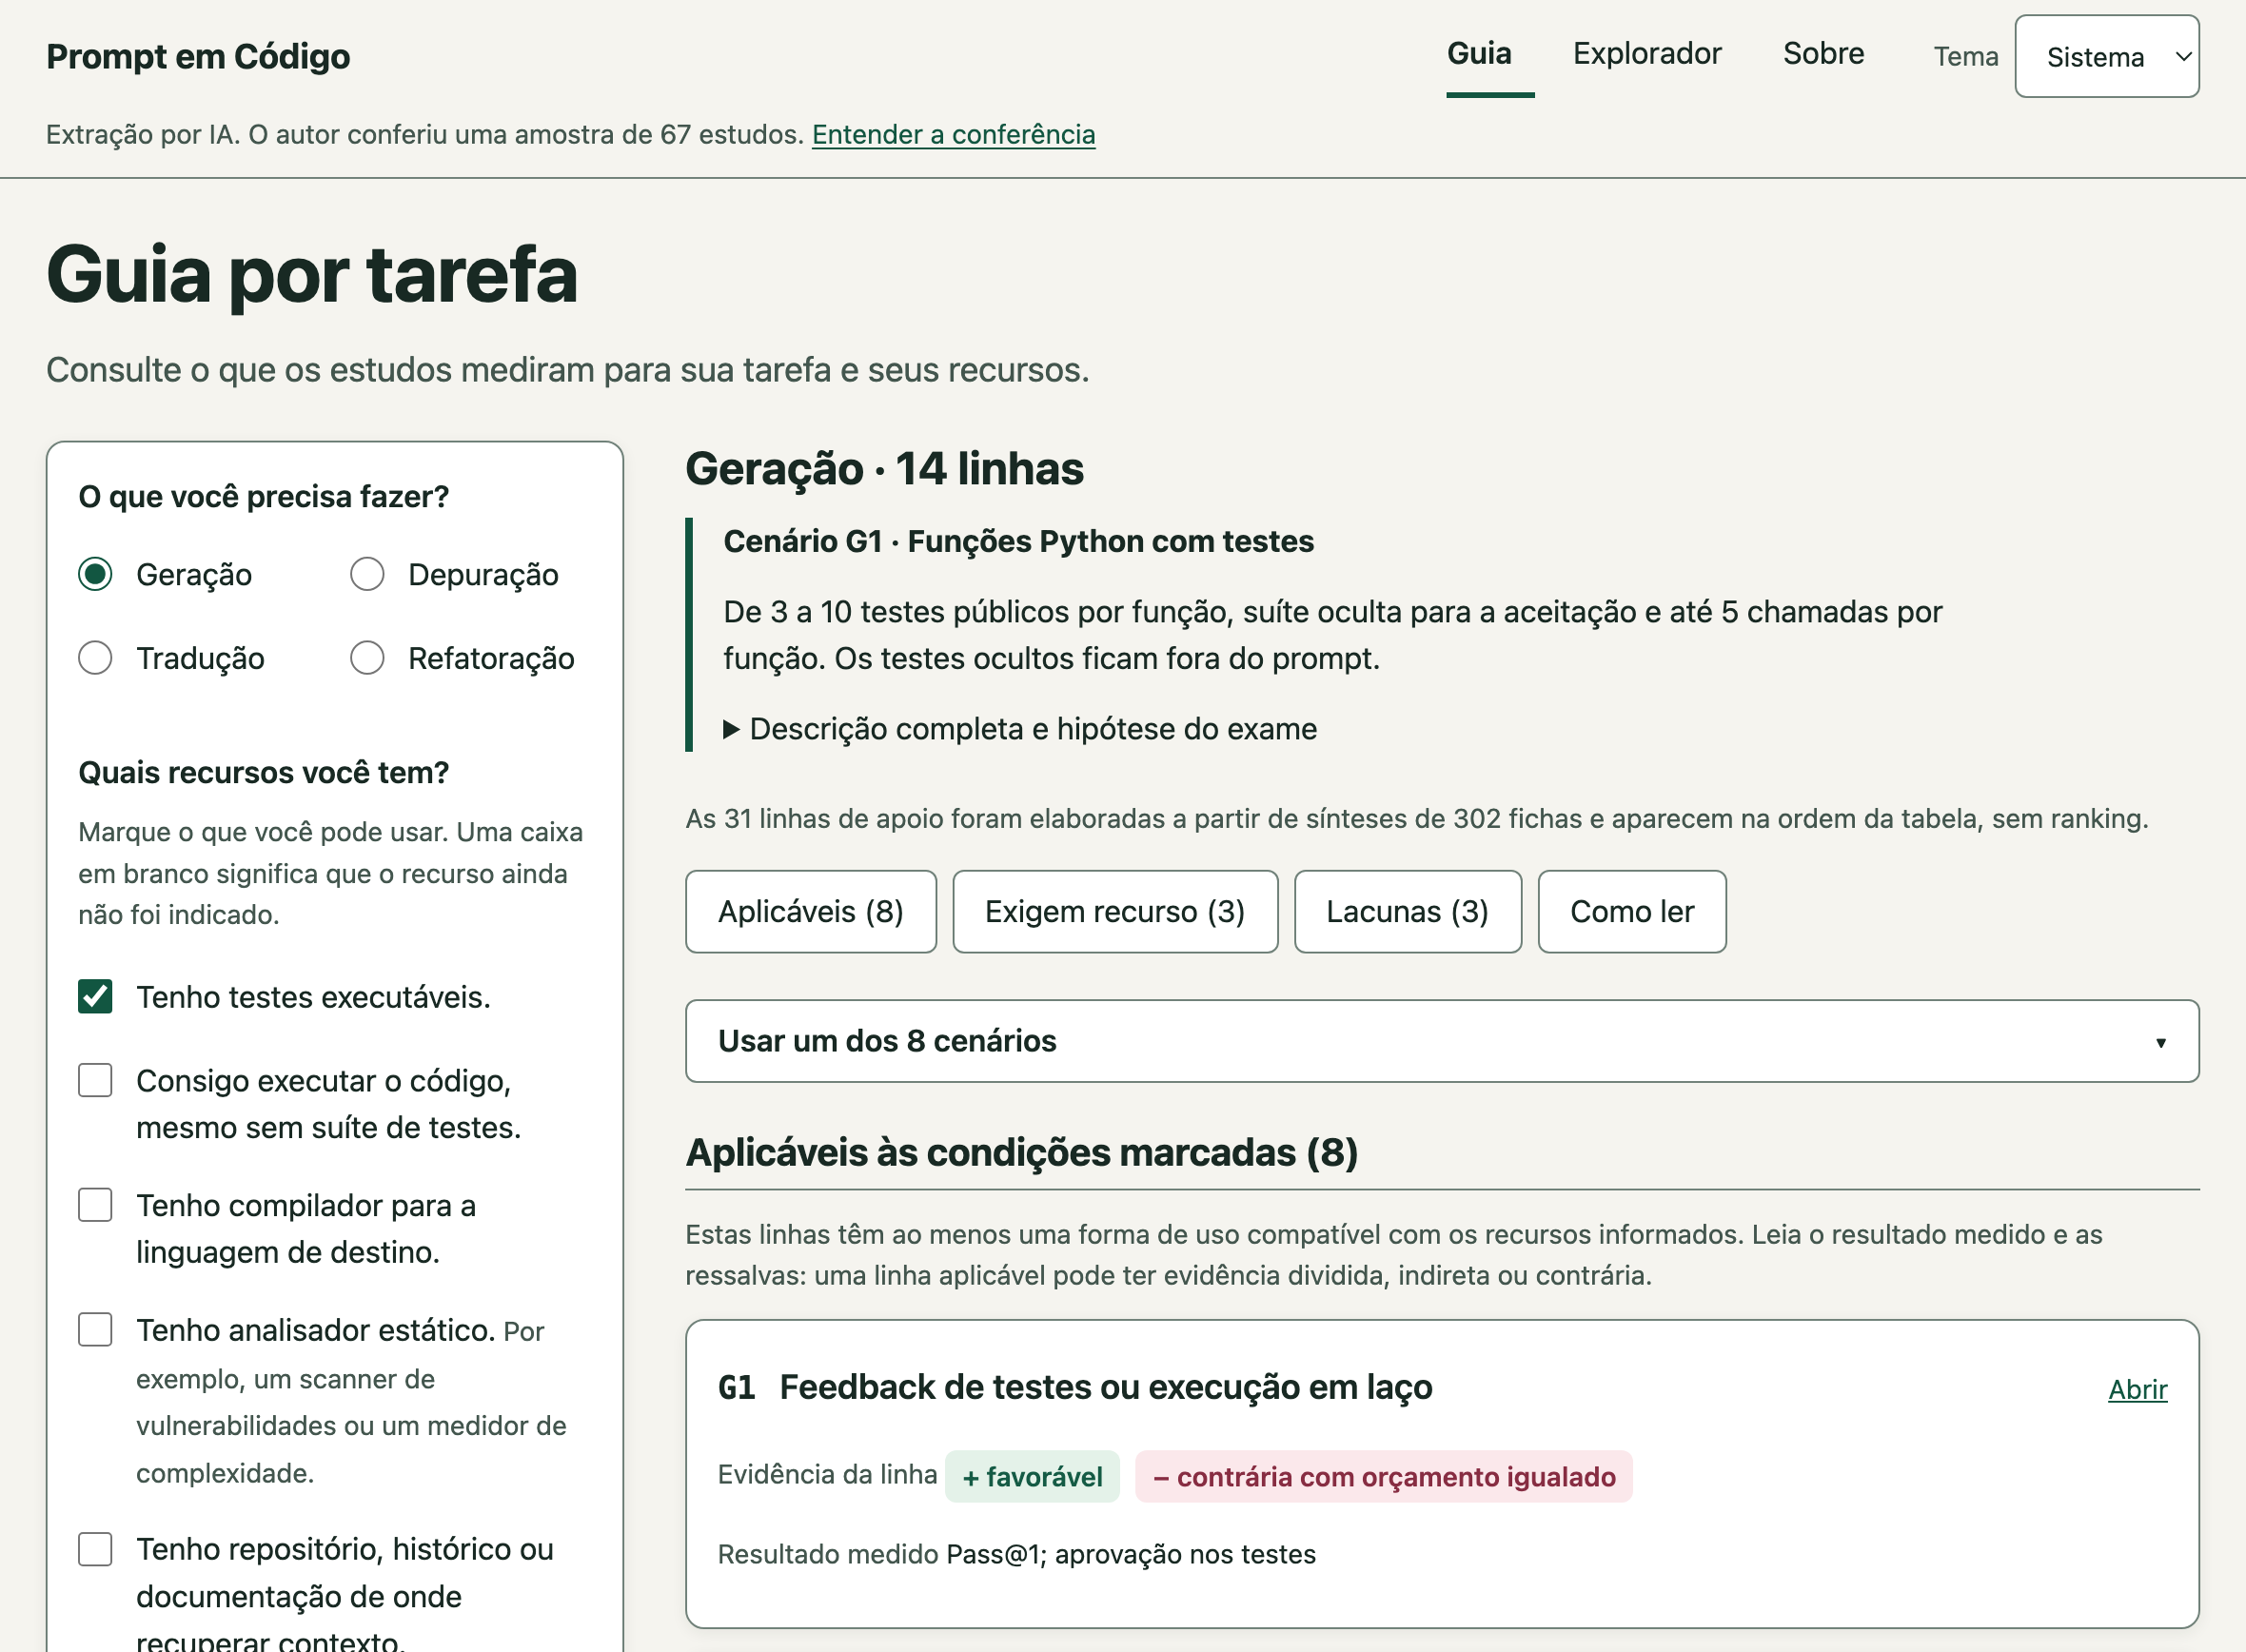
\includegraphics[width=\textwidth,height=0.42\textheight,keepaspectratio]{figuras/guia-cenario-g1}
\ifdefined\fontetabela\else\caption{Guide screen with the conditions of scenario G1, on 22 November 2026 (interface in Portuguese)}\label{fig:guia}\fi
\end{figure*}

The Explorer gives access to the 805 comparisons. The search looks up identifier, study title, technique,
comparator, model, benchmark and metric, and the filters select task, mechanism added and direction
of the comparison. A matrix shows the count of comparisons per mechanism added and task, and each cell opens
the corresponding list. The index of studies leads to the record of each of the 332 studies, with its techniques, its
comparisons and the address of the source, when recorded. The About screen summarizes the method, explains how to read the terms used and reports the
coverage of the data and the status of the check.

The system keeps the limits of the synthesis. The rows appear in the order of the table, without ranking and without averaging
across benchmarks, and each pair of values is presented separately. An applicable row is one whose
required resources were ticked, and its evidence may be mixed, indirect or contrary. Each comparison
states that the extraction was made by AI and whether it belongs to the sample checked by the author. The rows of the Guide come from the
syntheses of 302 records, and the later extractions appear only in the Explorer. The separation of the rows into the three
groups and the filling in of the scenarios were derived from the condition column of the table, with AI support, and do not yet
have a recorded review by the author. They are editorial decisions of the system, and not results of the review.

The design specification was made by Codex and the implementation, by Claude Code, AI assistants, at the request of the
author. The code, the data and the automated tests that compare the published file with the sources are in the
project repository. The verification consisted of these tests and of the inspection of the screens in the browser. The system was not
evaluated with users, and for this reason this work does not claim its usefulness or its usability.

\subsection{Comparison with other reviews}\label{sec:comparacao}
The general reviews of LLMs in software engineering describe which prompting techniques the studies use, but not
what each one adds to the prompt or under which condition it works. \citet{hou2024slr} count the frequency
of the techniques in studies up to January 2024. This work covers only four tasks, includes studies up to 2026 and
records, per comparison, the type of counterfactual, the direction and the conditions. This explains the main difference in
reading: most of the evidence is of packages against baselines, which a usage count does not show.

Two points converge with closely related reviews.
The role of verifiable external information, such as tests, execution and repository context, in the favourable
results of this corpus is consistent with the emphasis of \citet{fan2023survey} on hybrid techniques, which
combine traditional software engineering and LLMs.
% AFIRMACAO: A120
The dependence on perfect localization of the defect, recorded here in the debugging rows, also appears in
\citet{yang2025aprsurvey}, who record this assumption for each repair system, because it makes the
results hardly comparable across articles.
% AFIRMACAO: A122
On energy efficiency, \citet{masthanali2026energy} did not find a prompting strategy
that improves the result consistently, which resembles the mixed results of the instructions and of
self-critique without execution in this work.
% AFIRMACAO: A123

The reviews of prompting techniques, such as that of \citet{sahoo2024survey}, organize the techniques by area
and summarize the results reported by their authors, without crossing them with the evaluation conditions. The decision-support table
of this work tries to fill this gap for the four tasks, with the caveat that the search was not designed
to locate reviews and, therefore, no claim is made that the combination is new.

\subsection{Threats to validity}\label{sec:ameacas}
The threats below follow from the method carried out up to 17 November 2026.

\textit{Search coverage.} The search used three databases and a single search string, applied to title and abstract. The string
did not retrieve two of the six studies of the reference set (S3 and S5), because title and abstract do not combine the
three blocks of terms, which indicates a potential coverage limitation; the eligibility of these two studies was not
assessed. There was no broad snowballing to compensate.
The number of studies retrieved does not, by itself, demonstrate that the coverage is adequate.

\textit{Concessions of the rapid review.} Requiring the task in the title reduced the candidates from 2,304 to 715, but, in the
calibration samples, 46 of the 79 studies included by the author (58\%) did not have the task in the title and would be left
out (Section~\ref{sec:calibracao}). This is the main limitation of the work: the corpus represents the studies that
name the task in the title, and not the whole literature on the subject. The cut of stage 2 removes 233 studies available
only on arXiv, which tends to under-represent the most recent work, still without a reviewed publication.

\textit{Access to the texts.} The protocol started restricted to open access and came to accept the institutional access
of UFMG after the title and abstract screening. Studies outside the two types of access are not read. Stage 3,
almost all from IEEE Xplore, was read by the models and checked by the author in the 111 studies. IEEE Xplore studies
without institutional access and those only on arXiv (stage 2) remain outside the corpus of this version.

\textit{AI-assisted selection.} The screening was done by two models from the same vendor (Claude Opus 5.5 and Claude
Sonnet 5.5), which may err in the same way. For this reason, the agreement between them ($\kappa = 0.726$ at title and
abstract and $\kappa = 0.745$ in the 419 full-text studies) does not indicate correctness. The comparison with the author shows
relevant disagreements: at full text, with the author's first decision, $\kappa = 0.641$ with AI-A and
$0.548$ with AI-B. Of the 60 consensual exclusions at
full text, the author included 5, and, at title and abstract, 7 of the 92. Since the author checked all the consensual
exclusions in the two phases, these studies were not lost. The measure, however, shows that exclusion by two
models does not dispense with the human check. There is a single human reviewer, and not independent dual human
screening.

\textit{Application of the criteria.} The rule of I2 for the full text was defined after the calibration, and the boundary of
X4 for studies in which prompting is only a baseline was formulated during the check. Both were decided
in view of the data and may reflect the cases that motivated them. The boundary of X4 depends on judging whether a prompting result is
analysed as a finding or serves only as a reference, and this judgement may vary between readers; with a single
human reviewer, this variation was not measured. The boundary was applied to S314 and S373 on the basis of the reasons already
recorded, without a new reading. Of the nine studies in doubt, eight were excluded later, and one (S1617) was included by the
rule of the date of the event.

\textit{Reading from the extracted text.} The models read the text extracted from the PDFs, without figures and with tables sometimes
scrambled, returning to the PDF only in case of doubt. In three studies, one of the models read only part of the text, and
in seven long texts it was not verified whether the reading was complete. The author read all the 419 studies checked, which reduces,
but does not eliminate, the effect of these failures on the selection.

\textit{Extraction and synthesis.} The extraction was done by AI, with a single extractor per study. Two models
worked on the 332 records: Claude Opus 5.5 on 295 studies and Codex on 27, plus the 10 pilot records,
extracted by Opus. The calibration in the pilot
showed errors in reading values and in selecting comparisons, and does not estimate the error rate in new studies. The author checked the 67
studies of the sample after the synthesis and corrected 18 of 571 blocks (3.2\%), but 56 of these studies have only the
declaration that they were correct, without a record per block. The rate holds for the blocks judged; outside the sample, the records remain
as extraction by AI. The synthesis by grouping was drafted in a first
version by subagents, over excerpts of the records. The automatic check confirmed that the identifiers
cited exist, but not that each sentence reflects the study. The author checked each claim
against the original and marked 30 of the 120 for correction. The limit of three comparisons per study, chosen without looking at the effect, reduces selective choice in the
extraction, but leaves out results that the authors report in other tables. The heterogeneity recorded in a
targeted search compensates only in part for this loss. The studies use different models, benchmarks and
metrics, and for this reason the synthesis does not compute averages or rank techniques. Results on benchmarks do not,
by themselves, demonstrate gains in productivity, security or cost. They may be affected by contamination of the
training data, which 187 of the 332 studies with a record do not address.

\textit{Validation of the practical contribution.} The taxonomy and the decision-support table were examined in eight synthetic
scenarios, with judgement by the author, without external users or an experiment. This examination verifies clarity, grounding in the sources and concrete guidance, but
does not measure the effectiveness of the techniques or the usefulness of the table for developers. The system of
Section~\ref{sec:aplicacao} was also not evaluated with users.

\subsection{Social, economic and environmental impacts}
The studies of the corpus measure performance on benchmarks and, in few cases, cost or energy. The evidence on
the performance of developers is scarce: S62 measures time and accuracy of 20 participants in a delimited task of
reviewing patches, with and without explanations, with no significant difference in time (S62, section 5.4). These
results do not allow general productivity gains to be concluded, and for this reason this work does not claim economic
gains.

Among the impacts measured, multi-step techniques multiply calls and tokens. MapCoder, for
example, used on average 16.7 calls and 21.25 thousand tokens, against one call and 0.64 thousand tokens for the
direct prompt (S344).
% AFIRMACAO: A57
This cost also has an environmental dimension, since repair consumed from 5 to 15 times the energy of the single pass in
one study (S1415). Risks to the security of the code were also measured, such as the vulnerabilities introduced
or preserved in translation (S951) and those accumulated in improvement iterations (S739).
% AFIRMACAO: A50

The effects on those who use the techniques hardly appear in the records. One exception is the report of participants who
accepted without scrutiny the reasoning of incorrect patches (S62).
% AFIRMACAO: A60
This type of effect calls for more studies with users; the few present in the corpus, such as that of S62, cover delimited
tasks.

% English translation of capitulos/06-conclusao.tex, made by Claude Code (Claude Fable 5.2) on 24 November 2026.
% Pending review by the author. When the Portuguese file changes, update this one (scripts/verificar_traducao.py).
\section{Conclusion}
This work organized the evidence on prompting techniques for code generation, translation, refactoring and
debugging. To do so, it carried out a rapid literature review that started from 2,304 unique studies in three databases and reached a
corpus of 332 studies included by the author at full text, all with an extraction record. The results
answer the three research questions with a caveat that holds for the whole text: the extraction was done by AI,
and the author
checked 67 studies selected for the sample, in which 18 of 571 blocks required correction, and the 120 empirical claims against the original, of which 30 called for correction.

As for RQ1, the techniques evaluated combine mechanisms, and most of the evidence compares the complete technique with
a baseline. In the extracted comparisons, many favourable results involve verifiable external
information: tests,
execution, repository context and localization of the defect. These gains depend on conditions that are not always
repeated outside the study, such as available tests, more calls to the model or information taken from the reference
solution. Reasoning instructions, self-critique without execution, fixed examples and changes in wording had
mixed or unfavourable results, especially with small models and in repair.

As for RQ2, functional correctness is the most recorded risk, and passing tests is not always equivalent to correct
code. Almost all studies propose some mitigation, but fewer than half evaluate at least one. Contamination and
non-determinism are treated as design care, almost without evaluation, and security instructions may reduce
correctness.

As for RQ3, the multi-label taxonomy separates task, mechanism, role, type of counterfactual and conditions. The decision-support
table summarizes, per task and grouping, the direction of the comparisons, the strength of the evidence and the caveats. It also
marks the cases in which the evidence is not enough to recommend a technique.

In the examination in eight scenarios, the author judged the table partial on most criteria. It led to an executable
script only when the condition of the scenario coincided with that of the studies (D1), and did not declare the evidence
insufficient when reproduction of the defect or tests were missing (D2 and T2). For this reason, the author decided to revise it. Version 2
separates the types of verification, states the result measured in each row and declares in rows of their own the
conditions without sufficient evidence. The inclusion of stage 2 remains to be defined with the advisor.
Outside the sample, the records remain as extraction by AI. The
findings hold for this corpus, which contains only studies with the task in the title and an indication of peer review, and for
results on benchmarks. They do not demonstrate gains in productivity, security or cost in real use.


% Declarations required by the SBC Reviews template (English version of declaracoes.tex). Drafted by
% Claude Code (Claude Fable 5.2) on 24 November 2026 from what the repository documents (D143). They are
% declarations of the authors: they depend on confirmation by the three of them.
\begin{declarations}

\begin{contributions}
% Draft following the CRediT taxonomy, to be confirmed by the authors.
CCF defined the research questions, the criteria and the protocol, checked the search, screened the calibration samples,
checked the full-text reading decisions, the sample of extractions and the empirical claims in the text, and
is responsible for the content (conceptualization, methodology, investigation, validation and data curation). EMLF supervised the
work and PSCG co-supervised it (supervision). The participation of the AI tools is described in the declaration on the use
of artificial intelligence.
\end{contributions}

\begin{interests}
\pendencia{declaration of competing interests, to be made by the three authors.}
\end{interests}

\begin{materials}
The protocol and its changes, the exact queries for each database, the prompts, the data, the extraction records, the
scripts and the logs of decisions and of AI use created in this review are in the public project repository
(\url{https://github.com/caiofreitas1/tcc2-prompt-engineering}). The decision-support table and the extracted comparisons can
be consulted in the Prompt em Código system (\url{https://caiofreitas1.github.io/tcc2-prompt-engineering/}). The PDFs
and the texts extracted from the articles are not part of the repository.
\end{materials}

\begin{aitools}
This work used generative AI tools in the operation of the review and in the writing, as detailed in
Section~\ref{sec:ia}. Claude Code (Anthropic), with the models Claude Opus 5.5, Claude Sonnet 5.5 and Claude Fable 5.2,
carried out the search, the deduplication, the screening and the full-text reading, the extraction and the quality assessment, the
synthesis, the counts, the composition of the tables and the draft of the text. Codex CLI (OpenAI) took part in the extraction
and audited project materials. The check of the metadata of the references, the Prompt em Código system and the
adaptation to this format were also made with these tools. The text was written in Portuguese and translated into English
by Claude Code (Claude Fable 5.2); the translation has not yet been reviewed by the authors. The tables and the counts are generated by
scripts from the data in the repository. The steps checked by the author and the scope of each check are in
Section~\ref{sec:conferencia}. The authors are responsible for all the content.
\end{aitools}

\begin{furtherinformation}
This is a review of published studies. It did not involve human participants or personal data and was not submitted
to an ethics committee.
\pendencia{before submission: ORCID and institutional e-mail of Caio César de Freitas; e-mail of Pedro Saint Clair
Garcia; confirmation of the ORCIDs and of the e-mail obtained from public sources; choice of the corresponding author; approval of the
title in English; review of the translation by the authors; confirmation of the contributions and of the reading of the final version by the three authors; funding, if
any; and deposit of the artifacts with a persistent identifier and a licence, recommended by the journal.}
\end{furtherinformation}

\end{declarations}


\bibliographystyle{apalike-sol}
\bibliography{referencias}

% English translation of capitulos/07-apendice-busca.tex, made by Claude Code (Claude Fable 5.2) on 24 November 2026.
% Pending review by the author. When the Portuguese file changes, update this one (scripts/verificar_traducao.py).
\appendices
\section{Search string and filters}\label{ap:busca}
The general search string, applied to title and abstract, is:

{\footnotesize\raggedright
(``prompt engineering'' OR prompting OR prompt OR prompts OR ``in-context learning'' OR ``few-shot''
OR ``zero-shot'' OR ``chain-of-thought'' OR ``chain of thought'') AND (``code generation'' OR
``program synthesis'' OR ``code translation'' OR ``program translation'' OR ``code migration'' OR
transpil* OR refactoring OR refactor OR debugging OR debug OR ``program repair'' OR ``bug fixing'' OR
``bug fix'' OR ``bug repair'') AND (``large language model'' OR ``large language models'' OR LLM OR
LLMs OR ``language model'' OR ``language models'' OR ``generative AI'' OR ChatGPT OR ``GPT-4'' OR
Codex)\par}

\medskip
The filters applied were: on arXiv, submission date from 1 January 2021 to 7 September 2026; on IEEE Xplore,
years from 2021 to 2026; on the ACM Digital Library, electronic publication from January 2021 to September 2026, including the
whole month, in the ACM Full-Text collection. In the rapid review adopted, the block of tasks is applied only to the
title, by local simulation over the records, without a new search in the databases. The exact query for each database is in \texttt{dados/buscas.csv}, in the project repository.

% Generated by scripts/gerar_apendice_estudos.py (English text of capitulos/08-apendice-estudos.tex).
\section{Included studies}\label{ap:estudos}
The 332 studies of the definitive corpus, by the identifier used in the text. Title and identifier come from the database records; year and authorship were not checked for this list. The 67 studies marked with $\ast$ were read in the arXiv version; the identifier is that of the publication in a journal or in proceedings, located on 21 November 2026 by comparing the title and the authors with those of the arXiv record. Another 2 remain identified by arXiv, with no publication located.

{\scriptsize\raggedright
\begin{description}\setlength{\itemsep}{0pt}\setlength{\parskip}{0pt}
\item[S1$^\ast$] Self-planning Code Generation with Large Language Models. \texttt{doi:10.1145/3672456}.
\item[S4$^\ast$] An Empirical Study on the Code Refactoring Capability of Large Language Models. \texttt{doi:10.1145/3801158}.
\item[S6] Chain of Grounded Objectives: Concise Goal-Oriented Prompting for Code Generation. \texttt{doi:10.4230/LIPIcs.ECOOP.2025.35}.
\item[S14] A Neural Network Solves, Explains, and Generates University Math Problems by Program Synthesis and Few-Shot Learning at Human Level. \texttt{doi:10.1073/pnas.2123433119}.
\item[S25$^\ast$] Repair Is Nearly Generation: Multilingual Program Repair with LLMs. \texttt{doi:10.1609/aaai.v37i4.25642}.
\item[S50$^\ast$] ADELT: Transpilation Between Deep Learning Frameworks. \texttt{doi:10.24963/ijcai.2024/694}.
\item[S53] InferFix: End-to-End Program Repair with LLMs. \texttt{doi:10.1145/3611643.3613892}.
\item[S62$^\ast$] Explainable Automated Debugging via Large Language Model-driven Scientific Debugging. \texttt{doi:10.1007/s10664-024-10594-x}.
\item[S65$^\ast$] A study on Prompt Design, Advantages and Limitations of ChatGPT for Deep Learning Program Repair. \texttt{doi:10.1007/s10515-025-00492-x}.
\item[S77] Structured Chain-of-Thought Prompting for Code Generation. \texttt{doi:10.1145/3690635}.
\item[S90$^\ast$] Uncovering and Quantifying Social Biases in Code Generation. \texttt{doi:10.52202/075280-0110}.
\item[S109$^\ast$] Exploring and Characterizing Large Language Models For Embedded System Development and Debugging. \texttt{doi:10.1145/3613905.3650764}.
\item[S114] Franc: A Lightweight Framework for High-Quality Code Generation. \texttt{doi:10.1109/scam63643.2024.00020}.
\item[S120$^\ast$] Private-Library-Oriented Code Generation with Large Language Models. \texttt{doi:10.1016/j.knosys.2025.113934}.
\item[S124] An Empirical Study of the Non-determinism of ChatGPT in Code Generation. \texttt{doi:10.1145/3697010}.
\item[S129] Exploring Parameter-Efficient Fine-Tuning Techniques for Code Generation with Large Language Models. \texttt{doi:10.1145/3714461}.
\item[S137$^\ast$] BioCoder: A Benchmark for Bioinformatics Code Generation with Large Language Models. \texttt{doi:10.1093/bioinformatics/btae230}.
\item[S140] Bias Testing and Mitigation in LLM-based Code Generation. \texttt{doi:10.1145/3724117}.
\item[S149] From Misuse to Mastery: Enhancing Code Generation with Knowledge-Driven AI Chaining. \texttt{doi:10.1109/ase56229.2023.00143}.
\item[S150] Fixing Large Language Models' Specification Misunderstanding for Better Code Generation. \texttt{doi:10.1109/icse55347.2025.00108}.
\item[S170] Large Language Model-Aware In-Context Learning for Code Generation. \texttt{doi:10.1145/3715908}.
\item[S176] API-Assisted Code Generation for Question Answering on Varied Table Structures. \texttt{doi:10.18653/v1/2023.emnlp-main.897}.
\item[S193$^\ast$] Explain-then-Translate: An Analysis on Improving Program Translation with Self-generated Explanations. \texttt{doi:10.18653/v1/2023.findings-emnlp.119}.
\item[S195] Bring Your Own KG: Self-Supervised Program Synthesis for Zero-Shot KGQA. \texttt{doi:10.18653/v1/2024.findings-naacl.57}.
\item[S202] Refactoring Programs Using Large Language Models with Few-Shot Examples. \texttt{doi:10.1109/apsec60848.2023.00025}.
\item[S207] Novel Preprocessing Technique for Data Embedding in Engineering Code Generation Using Large Language Model. \texttt{doi:10.1109/lad62341.2024.10691715}.
\item[S213] On the Effectiveness of Large Language Models in Domain-Specific Code Generation. \texttt{doi:10.1145/3697012}.
\item[S216] Chain-of-Thought in Neural Code Generation: From and for Lightweight Language Models. \texttt{doi:10.1109/tse.2024.3440503}.
\item[S233$^\ast$] DebugBench: Evaluating Debugging Capability of Large Language Models. \texttt{doi:10.18653/v1/2024.findings-acl.247}.
\item[S247] Knowledge-Aware Code Generation with Large Language Models. \texttt{doi:10.1145/3643916.3644418}.
\item[S261] MPIrigen: MPI Code Generation through Domain-Specific Language Models. \texttt{doi:10.1145/3660605.3660944}.
\item[S271$^\ast$] HumanEval-XL: A Multilingual Code Generation Benchmark for Cross-lingual Natural Language Generalization. \texttt{doi:10.63317/2zjsm6sdd5yo}.
\item[S273] Compositional API Recommendation for Library-Oriented Code Generation. \texttt{doi:10.1145/3643916.3644403}.
\item[S275] When Large Language Models Confront Repository-Level Automatic Program Repair: How Well They Done?. \texttt{doi:10.1145/3639478.3647633}.
\item[S279$^\ast$] Design2Code: Benchmarking Multimodal Code Generation for Automated Front-End Engineering. \texttt{doi:10.18653/v1/2025.naacl-long.199}.
\item[S282$^\ast$] Guiding Enumerative Program Synthesis with Large Language Models. \texttt{doi:10.1007/978-3-031-65630-9\_15}.
\item[S295$^\ast$] Exploring Language Model's Code Generation Ability with Auxiliary Functions. \texttt{doi:10.18653/v1/2024.findings-naacl.181}.
\item[S301] SOEN-101: Code Generation by Emulating Software Process Models Using Large Language Model Agents. \texttt{doi:10.1109/icse55347.2025.00140}.
\item[S302$^\ast$] Iterative Refinement of Project-Level Code Context for Precise Code Generation with Compiler Feedback. \texttt{doi:10.18653/v1/2024.findings-acl.138}.
\item[S303] RepairAgent: An Autonomous, LLM-Based Agent for Program Repair. \texttt{doi:10.1109/icse55347.2025.00157}.
\item[S304] Output Format Biases in the Evaluation of Large Language Models for Code Translation. \texttt{doi:10.1145/3650105.3652301}.
\item[S309] Assessing, Exploiting, and Mitigating Syntactic Robustness Failures in LLM-Based Code Generation. \texttt{doi:10.1145/3793655.3793727}.
\item[S315] The Fact Selection Problem in LLM-Based Program Repair. \texttt{doi:10.1109/icse55347.2025.00162}.
\item[S319$^\ast$] Comments as Natural Logic Pivots: Improve Code Generation via Comment Perspective. \texttt{doi:10.18653/v1/2024.findings-acl.420}.
\item[S320] CreativEval: Evaluating Creativity of LLM-Based Hardware Code Generation. \texttt{doi:10.1109/lad62341.2024.10691798}.
\item[S321] Aligning the Objective of LLM-Based Program Repair. \texttt{doi:10.1109/icse55347.2025.00169}.
\item[S323] The Fault in our Stars: Quality Assessment of Code Generation Benchmarks. \texttt{doi:10.1109/scam63643.2024.00028}.
\item[S325$^\ast$] Low-Cost Language Models: Survey and Performance Evaluation on Python Code Generation. \texttt{doi:10.1016/j.engappai.2024.109490}.
\item[S328$^\ast$] Assessing GPT-4-Vision's Capabilities in UML-Based Code Generation. \texttt{doi:10.1145/3643795.3648391}.
\item[S329] Exploring and Unleashing the Power of Large Language Models in Automated Code Translation. \texttt{doi:10.1145/3660778}.
\item[S342] MEIC: Re-Thinking RTL Debug Automation Using LLMs. \texttt{doi:10.1145/3676536.3676801}.
\item[S344$^\ast$] MapCoder: Multi-Agent Code Generation for Competitive Problem Solving. \texttt{doi:10.18653/v1/2024.acl-long.269}.
\item[S348$^\ast$] AnalogCoder: Analog Circuit Design via Training-Free Code Generation. \texttt{doi:10.1609/aaai.v39i1.32016}.
\item[S354$^\ast$] LeDex: Training LLMs to Better Self-Debug and Explain Code. \texttt{doi:10.52202/079017-1120}.
\item[S357$^\ast$] DevEval: A Manually-Annotated Code Generation Benchmark Aligned with Real-World Code Repositories. \texttt{doi:10.18653/v1/2024.findings-acl.214}.
\item[S360] CatCoder: Repository-Level Code Generation with Relevant Code and Type Context. \texttt{doi:10.1145/3779217}.
\item[S361] VHDL-Eval: A Framework for Evaluating Large Language Models in VHDL Code Generation. \texttt{doi:10.1109/lad62341.2024.10691836}.
\item[S362] Refactoring to Pythonic Idioms: A Hybrid Knowledge-Driven Approach Leveraging Large Language Models. \texttt{doi:10.1145/3643776}.
\item[S365] JavaBench: A Benchmark of Object-Oriented Code Generation for Evaluating Large Language Models. \texttt{doi:10.1145/3691620.3695470}.
\item[S383$^\ast$] Retrieval-Augmented Code Generation for Situated Action Generation: A Case Study on Minecraft. \texttt{doi:10.18653/v1/2024.findings-emnlp.652}.
\item[S391$^\ast$] Toward Secure Code Generation: Bridging Correctness and Security via Task-Adaptive Vulnerability Modeling and Execution-Based Benchmarking. \texttt{doi:10.1145/3832159}.
\item[S393] Automated C/C++ Program Repair for High-Level Synthesis via Large Language Models. \texttt{doi:10.1109/mlcad62225.2024.10740262}.
\item[S397] Prompting Techniques for Secure Code Generation: A Systematic Investigation. \texttt{doi:10.1145/3722108}.
\item[S398$^\ast$] On Leakage of Code Generation Evaluation Datasets. \texttt{doi:10.18653/v1/2024.findings-emnlp.772}.
\item[S399$^\ast$] Benchmarking Language Model Creativity: A Case Study on Code Generation. \texttt{doi:10.18653/v1/2025.naacl-long.141}.
\item[S409] Enhancing Code Translation in Language Models with Few-Shot Learning via Retrieval-Augmented Generation. \texttt{doi:10.1109/hpec62836.2024.10938485}.
\item[S412] ThinkRepair: Self-Directed Automated Program Repair. \texttt{doi:10.1145/3650212.3680359}.
\item[S414] TaskEval: Assessing Difficulty of Code Generation Tasks for Large Language Models. \texttt{doi:10.1145/3773285}.
\item[S416$^\ast$] ArchCode: Incorporating Software Requirements in Code Generation with Large Language Models. \texttt{doi:10.18653/v1/2024.acl-long.730}.
\item[S427$^\ast$] An Exploratory Study on Fine-Tuning Large Language Models for Secure Code Generation. \texttt{doi:10.1007/s10664-026-10803-9}.
\item[S429] Bridging the Language Gap: Enhancing Multilingual Prompt-Based Code Generation in LLMs via Zero-Shot Cross-Lingual Transfer. \texttt{doi:10.1109/ijcnn64981.2025.11227991}.
\item[S432] Revisiting VerilogEval: A Year of Improvements in Large-Language Models for Hardware Code Generation. \texttt{doi:10.1145/3718088}.
\item[S435] Enhancing Automated Program Repair with Solution Design. \texttt{doi:10.1145/3691620.3695537}.
\item[S447$^\ast$] Can OpenSource beat ChatGPT? -- A Comparative Study of Large Language Models for Text-to-Code Generation. \texttt{aclanthology.org/2024.swisstext-1.1}.
\item[S448] A Pair Programming Framework for Code Generation via Multi-Plan Exploration and Feedback-Driven Refinement. \texttt{doi:10.1145/3691620.3695506}.
\item[S459] Contextualized Data-Wrangling Code Generation in Computational Notebooks. \texttt{doi:10.1145/3691620.3695503}.
\item[S466] Automated Unit Test Refactoring. \texttt{doi:10.1145/3715750}.
\item[S479$^\ast$] What Makes Large Language Models Reason in (Multi-Turn) Code Generation?. International Conference on Learning Representations (ICLR 2025).
\item[S491$^\ast$] Personality-Guided Code Generation Using Large Language Models. \texttt{doi:10.18653/v1/2025.acl-long.54}.
\item[S492] Agents4PLC: Automating Closed-Loop PLC Code Generation and Verification in Industrial Control Systems Using LLM-Based Agents. \texttt{doi:10.1109/tse.2026.3667895}.
\item[S495] mHumanEval -- A Multilingual Benchmark to Evaluate Large Language Models for Code Generation. \texttt{doi:10.18653/v1/2025.naacl-long.570}.
\item[S499] Less Is More: DocString Compression in Code Generation. \texttt{doi:10.1145/3735636}.
\item[S500] Demo-Craft: Using In-Context Learning to Improve Code Generation in Large Language Models. \texttt{doi:10.1109/iitcee64140.2025.10915349}.
\item[S501] Leveraging Large Language Models for Code Translation and Software Development in Scientific Computing. \texttt{doi:10.1145/3732775.3733572}.
\item[S508] Interaction2Code: Benchmarking MLLM-based Interactive Webpage Code Generation from Interactive Prototyping. \texttt{doi:10.1109/ase63991.2025.00028}.
\item[S511] An Empirical Study on the Potential of LLMs in Automated Software Refactoring. \texttt{doi:10.1007/s10515-025-00500-0}.
\item[S512] The First Prompt Counts the Most! An Evaluation of Large Language Models on Iterative Example-Based Code Generation. \texttt{doi:10.1145/3728947}.
\item[S530] DRC-Coder: Automated DRC Checker Code Generation Using LLM Autonomous Agent. \texttt{doi:10.1145/3698364.3705347}.
\item[S547$^\ast$] PERC: Plan-As-Query Example Retrieval for Underrepresented Code Generation. \texttt{aclanthology.org/2025.coling-main.534}.
\item[S552$^\ast$] Counterexample Guided Program Repair Using Zero-Shot Learning and MaxSAT-based Fault Localization. \texttt{doi:10.1609/aaai.v39i1.32046}.
\item[S553] Tree-of-Code: A Tree-Structured Exploring Framework for End-to-End Code Generation and Execution in Complex Task Handling. \texttt{arXiv:2412.15305}.
\item[S556] Top General Performance = Top Domain Performance? DomainCodeBench: A Multi-domain Code Generation Benchmark. \texttt{doi:10.1145/3744916.3773271}.
\item[S560] The Impact of Prompt Programming on Function-Level Code Generation. \texttt{doi:10.1109/tse.2025.3587794}.
\item[S569] HaVen: Hallucination-Mitigated LLM for Verilog Code Generation Aligned with HDL Engineers. \texttt{doi:10.23919/date64628.2025.10993072}.
\item[S570$^\ast$] Online Prompt Selection for Program Synthesis. \texttt{doi:10.1609/aaai.v39i11.33227}.
\item[S579] Testing Refactoring Engine via Historical Bug Report driven LLM. \texttt{doi:10.1109/forge66646.2025.00020}.
\item[S582] VRank: Enhancing Verilog Code Generation from Large Language Models via Self-Consistency. \texttt{doi:10.1109/isqed65160.2025.11014398}.
\item[S588$^\ast$] GLLM: Self-Corrective G-Code Generation using Large Language Models with User Feedback. \texttt{doi:10.18420/btw2025-29}.
\item[S591] Enhancing Code Generation for Low-Resource Languages: No Silver Bullet. \texttt{doi:10.1109/icpc66645.2025.00058}.
\item[S597] COFFE: A Code Efficiency Benchmark for Code Generation. \texttt{doi:10.1145/3715727}.
\item[S603$^\ast$] CodeSCM: Causal Analysis for Multi-Modal Code Generation. \texttt{doi:10.18653/v1/2025.naacl-long.345}.
\item[S604] Benchmarking Prompt Engineering Techniques for Secure Code Generation with GPT Models. \texttt{doi:10.1109/forge66646.2025.00018}.
\item[S613] Knowledge-Enhanced Program Repair for Data Science Code. \texttt{doi:10.1109/icse55347.2025.00246}.
\item[S629$^\ast$] Program Synthesis Dialog Agents for Interactive Decision-Making. \texttt{doi:10.18653/v1/2025.ijcnlp-long.176}.
\item[S633$^\ast$] CodeArena: A Collective Evaluation Platform for LLM Code Generation. \texttt{doi:10.18653/v1/2025.acl-demo.48}.
\item[S634] Code-as-Symbolic-Planner: Foundation Model-Based Robot Planning via Symbolic Code Generation. \texttt{doi:10.1109/iros60139.2025.11247174}.
\item[S641] Evaluating Large Language Models in Code Generation: INFINITE Methodology for Defining the Inference Index. \texttt{doi:10.3390/app15073784}.
\item[S645] Fully Autonomous Programming using Iterative Multi-Agent Debugging with Large Language Models. \texttt{doi:10.1145/3719351}.
\item[S647] Evaluating the Generalizability of LLMs in Automated Program Repair. \texttt{doi:10.1109/icse-nier66352.2025.00024}.
\item[S650] Prompt Alchemy: Automatic Prompt Refinement for Enhancing Code Generation. \texttt{doi:10.1109/tse.2025.3589634}.
\item[S654$^\ast$] MoT: Modularization-of-Thought Prompting for Effective Code Generation. \texttt{doi:10.1145/3832173}.
\item[S667] Smoke and Mirrors: Jailbreaking LLM-based Code Generation via Implicit Malicious Prompts. \texttt{doi:10.1145/3744916.3764566}.
\item[S670] What to Retrieve for Effective Retrieval-Augmented Code Generation? An Empirical Study and Beyond. \texttt{doi:10.1145/3744916.3773224}.
\item[S674] Post-Incorporating Code Structural Knowledge into Pretrained Models via ICL for Code Translation. \texttt{doi:10.1109/tse.2025.3605768}.
\item[S692] Enhancing LLM-Based Quantum Code Generation with Multi-Agent Optimization and Quantum Error Correction. \texttt{doi:10.1109/dac63849.2025.11133316}.
\item[S695] Give LLMs a Security Course: Securing Retrieval-Augmented Code Generation via Knowledge Injection. \texttt{doi:10.1145/3719027.3765049}.
\item[S699] Towards Adaptive Software Agents for Debugging. \texttt{doi:10.1145/3696630.3728514}.
\item[S703$^\ast$] A Multi-Language Perspective on the Robustness of LLM Code Generation. \texttt{doi:10.1007/s10664-026-10882-8}.
\item[S715$^\ast$] Towards Effectively Leveraging Execution Traces for Program Repair with Code LLMs. \texttt{doi:10.18653/v1/2025.knowledgenlp-1.17}.
\item[S724] Automated Repair of Ambiguous Problem Descriptions for LLM-Based Code Generation. \texttt{doi:10.1109/ase63991.2025.00038}.
\item[S732] SafeTrans: LLM-assisted Transpilation from C to Rust. \texttt{doi:10.1145/3786180.3788317}.
\item[S739] Security Degradation in Iterative AI Code Generation: A Systematic Analysis of the Paradox. \texttt{doi:10.1109/istas65609.2025.11269659}.
\item[S740$^\ast$] CLEVER: A Curated Benchmark for Formally Verified Code Generation. \texttt{doi:10.52202/085713-3857}.
\item[S755] GUARD:Dual-Agent based Backdoor Defense on Chain-of-Thought in Neural Code Generation. \texttt{doi:10.18293/seke2025-018}.
\item[S759$^\ast$] Self-Correcting Code Generation Using Small Language Models. \texttt{doi:10.18653/v1/2025.findings-emnlp.127}.
\item[S760] Enhancing LLM-Based Code Generation with Complexity Metrics: A Feedback-Driven Approach. \texttt{doi:10.1109/compsac65507.2025.00178}.
\item[S771] ScaleRTL: Scaling LLMs with Reasoning Data and Test-Time Compute for Accurate RTL Code Generation. \texttt{doi:10.1109/mlcad65511.2025.11189212}.
\item[S782] Code Roulette: How Prompt Variability Affects LLM Code Generation. \texttt{doi:10.1145/3786181.3788724}.
\item[S783] ExpeRepair: Dual-Memory Enhanced LLM-Based Repository-Level Program Repair. \texttt{doi:10.1145/3808181}.
\item[S795] Spec2RTL-Agent: Automated Hardware Code Generation from Complex Specifications Using LLM Agent Systems. \texttt{doi:10.1109/iclad65226.2025.00013}.
\item[S799] Automatic Qiskit Code Refactoring Using Large Language Models. \texttt{doi:10.1109/chilecon66915.2025.11476424}.
\item[S800] TeXpert: A Multi-Level Benchmark for Evaluating LaTeX Code Generation by LLMs. \texttt{doi:10.18653/v1/2025.sdp-1.2}.
\item[S806] QHackBench: Benchmarking Large Language Models for Quantum Code Generation Using PennyLane Hackathon Challenges. \texttt{doi:10.1109/qai63978.2025.00056}.
\item[S810] T3: Multi-level Tree-based Automatic Program Repair with Large Language Models. \texttt{doi:10.1109/ijcnn64981.2025.11228000}.
\item[S821] Hierarchical Knowledge Injection for Improving LLM-based Program Repair. \texttt{doi:10.1109/ase63991.2025.00122}.
\item[S834] Are They All Good? Evaluating the Quality of CoTs in LLM-Based Code Generation. \texttt{doi:10.1109/tse.2026.3676295}.
\item[S836] NL in the Middle: Code Translation with LLMs and Intermediate Representations. \texttt{doi:10.1109/cascon66301.2025.00037}.
\item[S842] SIMCODE: A Benchmark for Natural Language to ns-3 Network Simulation Code Generation. \texttt{doi:10.1109/lcn65610.2025.11146057}.
\item[S845] Chain-of-Descriptions: Improving Code LLMs for VHDL Code Generation and Summarization. \texttt{doi:10.1145/3670474.3685966}.
\item[S852] RepoScope: Leveraging Call Chain-Aware Multi-View Context for Repository-Level Code Generation. \texttt{doi:10.1145/3744916.3773211}.
\item[S855] Input Reduction Enhanced LLM-based Program Repair. \texttt{doi:10.1145/3744916.3787760}.
\item[S878$^\ast$] ITUNLP at SemEval-2025 Task 8: Question-Answering over Tabular Data: A Zero-Shot Approach using LLM-Driven Code Generation. \texttt{aclanthology.org/2025.semeval-1.198}.
\item[S887] Data Dependency-Aware Code Generation from Enhanced UML Sequence Diagrams. \texttt{doi:10.1109/ase63991.2025.00282}.
\item[S892$^\ast$] More Than a Score: Probing the Impact of Prompt Specificity on LLM Code Generation. \texttt{doi:10.18653/v1/2025.ijcnlp-long.128}.
\item[S895] Experimental Analysis of Productive Interaction Strategy with ChatGPT: User Study on Function and Project-level Code Generation Tasks. \texttt{doi:10.1145/3844949}.
\item[S902] What Makes In-Context Examples Effective for Code Generation?. \texttt{doi:10.1145/3832275}.
\item[S910$^\ast$] LyS at SemEval 2025 Task 8: Zero-Shot Code Generation for Tabular QA. \texttt{aclanthology.org/2025.semeval-1.171}.
\item[S917] Hallucination in LLM-Based Code Generation: An Automotive Case Study. \texttt{doi:10.1109/fllm67465.2025.11391125}.
\item[S919$^\ast$] TRACE: Evaluating Execution Efficiency of LLM-Based Code Translation. \texttt{doi:10.18653/v1/2026.acl-long.140}.
\item[S939] Model-Driven Quantum Code Generation Using Large Language Models and Retrieval-Augmented Generation. \texttt{doi:10.1109/models67397.2025.00031}.
\item[S951] When Code Crosses Borders: A Security-Centric Study of LLM-based Code Translation. \texttt{doi:10.1109/tifs.2026.3746885}.
\item[S957$^\ast$] Quality Assessment of Tabular Data using Large Language Models and Code Generation. \texttt{doi:10.18653/v1/2025.emnlp-industry.183}.
\item[S958] Toward Green Code: Prompting Small Language Models for Energy-Efficient Code Generation. \texttt{doi:10.1109/fllm67465.2025.11391183}.
\item[S964] UniPar: A Unified LLM-Based Framework for Parallel and Accelerated Code Translation in HPC. \texttt{doi:10.1109/hpec67600.2025.11196677}.
\item[S979] RelRepair: Enhancing Automated Program Repair by Retrieving Relevant Code. \texttt{doi:10.1109/tr.2026.3736386}.
\item[S996] SolContractEval: A Benchmark for Evaluating Contract-Level Solidity Code Generation. \texttt{doi:10.1109/ase63991.2025.00235}.
\item[S1008] Automated Program Repair of Uncompilable Student Code. \texttt{doi:10.1145/3770761.3777323}.
\item[S1010] RustAssure: Differential Symbolic Testing for LLM-Transpiled C-to-Rust Code. \texttt{doi:10.1109/ase63991.2025.00051}.
\item[S1023] EvoCAD: Evolutionary CAD Code Generation with Vision Language Models. \texttt{doi:10.1109/ictai66417.2025.00075}.
\item[S1024$^\ast$] ContractEval: A Benchmark for Evaluating Contract-Satisfying Assertions in Code Generation. \texttt{doi:10.18653/v1/2026.findings-acl.2112}.
\item[S1032] When Many-Shot Prompting Fails: An Empirical Study of LLM Code Translation. \texttt{doi:10.1145/3786180.378831}.
\item[S1034] SEER: Enhancing Chain-of-Thought Code Generation through Self-Exploring Deep Reasoning. \texttt{doi:10.1145/3744916.3773197}.
\item[S1047$^\ast$] Once Upon an Input: Reasoning via Per-Instance Program Synthesis. \texttt{doi:10.52202/085713-4571}.
\item[S1053$^\ast$] SymCode: A Neurosymbolic Approach to Mathematical Reasoning via Verifiable Code Generation. \texttt{doi:10.18653/v1/2026.findings-eacl.76}.
\item[S1054] Automated Extract Method Refactoring with Open-Source LLMs: A Comparative Study. \texttt{doi:10.1109/aiware69974.2025.00020}.
\item[S1065] Secure Code Generation at Scale with Reflexion. \texttt{doi:10.1109/aiware69974.2025.00038}.
\item[S1070] OUNLP at TSAR 2025 Shared Task: Multi-Round Text Simplifier via Code Generation. \texttt{doi:10.18653/v1/2025.tsar-1.19}.
\item[S1074] UA-Code-Bench: A Competitive Programming Benchmark for Evaluating LLM Code Generation in Ukrainian. \texttt{doi:10.15276/ict.02.2025.47}.
\item[S1077$^\ast$] Retriv at BLP-2025 Task 2: Test-Driven Feedback-Guided Framework for Bangla-to-Python Code Generation. \texttt{doi:10.18653/v1/2025.banglalp-1.59}.
\item[S1080] Vendor-Aware Industrial Agents: RAG-Enhanced LLMs for Secure On-Premise PLC Code Generation. \texttt{doi:10.1109/icit64854.2026.11491098}.
\item[S1086$^\ast$] Enhancing LLM Code Generation Capabilities through Test-Driven Development and Code Interpreter. \texttt{doi:10.18653/v1/2025.banglalp-1.56}.
\item[S1107$^\ast$] PyBangla at BLP-2025 Task 2: Enhancing Bangla-to-Python Code Generation with Iterative Self-Correction and Multilingual Agents. \texttt{doi:10.18653/v1/2025.banglalp-1.55}.
\item[S1121$^\ast$] Understanding Chain-of-Thought Effectiveness in Code Generation: An Empirical and Information-Theoretic Analysis. \texttt{doi:10.1007/s10664-026-10947-8}.
\item[S1132] Workflows vs Agents for Code Translation. \texttt{arXiv:2512.14762}.
\item[S1133$^\ast$] Intention Chain-of-Thought Prompting with Dynamic Routing for Code Generation. \texttt{doi:10.1609/aaai.v40i1.37030}.
\item[S1141] Comment Traps: How Defective Commented-out Code Augment Defects in AI-Assisted Code Generation. \texttt{doi:10.1145/3797102}.
\item[S1155] In Line with Context: Repository-Level Code Generation via Context Inlining. \texttt{doi:10.1145/3797094}.
\item[S1163$^\ast$] ParaCodex: A Profiling-Guided Autonomous Coding Agent for Reliable Parallel Code Generation and Translation. \texttt{doi:10.18653/v1/2026.acl-long.732}.
\item[S1176] Guidelines to Prompt Large Language Models for Code Generation: An Empirical Characterization. \texttt{doi:10.1145/3794763.3794819}.
\item[S1179] HardSecBench: Benchmarking the Security Awareness of LLMs for Hardware Code Generation. \texttt{doi:10.24963/ijcai.2026/57}.
\item[S1195$^\ast$] RealSec-bench: A Benchmark for Evaluating Secure Code Generation in Real-World Repositories. \texttt{doi:10.18653/v1/2026.findings-acl.1786}.
\item[S1204] Failure-Aware Enhancements for Large Language Model (LLM) Code Generation: An Empirical Study on Decision Framework. \texttt{doi:10.1109/saner67736.2026.00085}.
\item[S1220] JMigBench: A Benchmark for Evaluating LLMs on Source Code Migration (Java 8 to Java 11). \texttt{doi:10.1145/3786180.3788316}.
\item[S1229] SimulatorCoder: DNN Accelerator Simulator Code Generation and Optimization Via Large Language Models. \texttt{doi:10.1109/icassp55912.2026.11463415}.
\item[S1234$^\ast$] From Prompts to Performance: Evaluating LLMs for Task-based Parallel Code Generation. \texttt{doi:10.1007/978-3-032-27676-6\_2}.
\item[S1286] DePro: Understanding the Role of LLMs in Debugging Competitive Programming Code. \texttt{doi:10.1145/3803437.3805561}.
\item[S1304] From Guessing to Seeing: Enhancing LLM-Based Program Repair via Trace-Guided Multi-strategy Debate. \texttt{doi:10.1145/3832783.3837458}.
\item[S1359] Beyond Translation Accuracy: Addressing False Failures in LLM-Based Code Translation. \texttt{doi:10.1145/3805760.3814890}.
\item[S1368] Patterns of Developer Adoption of LLM-Generated Code Refactoring Suggestions. \texttt{doi:10.1145/3803846.3807462}.
\item[S1415] Knowledge boundary probing and demand-guided intervention for LLM-based power system code generation. \texttt{doi:10.1016/j.aei.2026.105328}.
\item[S1429] QBugLM: An Agentic Benchmarking Framework for LLM-based Quantum Software Debugging. \texttt{doi:10.1109/qsw72780.2026.00028}.
\item[S1450] No Resource, No Benchmarks, No Problem? Evaluating and Improving LLMs for Code Generation in No-Resource Languages. \texttt{doi:10.1109/tse.2026.3703553}.
\item[S1458$^\ast$] Text2DSL: LLM-Based Code Generation for Domain-Specific Languages. \texttt{doi:10.1016/j.procs.2026.09.361}.
\item[S1502$^\ast$] PROBE: Benchmarking Code Generation in Large Language Models. \texttt{doi:10.1007/s10664-026-10904-5}.
\item[S1503$^\ast$] Large Language Models for Code Generation from Multilingual Prompts: A Curated Benchmark and a Study on Code Quality. \texttt{doi:10.1145/3845994}.
\item[S1556] Do Influence Tactics Matter? Investigating Prompt Framing Effects in LLM Code Generation. \texttt{doi:10.1007/s10664-026-10934-z}.
\item[S1562$^\ast$] TDD-Agent: Test-Driven Reasoning for Code Generation. \texttt{doi:10.18653/2026.emnlp-main.1845}.
\item[S1565] XRFix: Exploring Performance Bug Repair of Extended Reality Applications with Large Language Models. \texttt{doi:10.1145/3744916.3773120}.
\item[S1583$^\ast$] Towards Fully Automated Medical Imaging Code Generation via Validation-based Context Engineering. \texttt{doi:10.1145/3832783.3834399}.
\item[S1592$^\ast$] TIPCODER: Reinforcement Learning Boosted Test-time Instruction Proposer for Code Generation. \texttt{doi:10.18653/2026.findings-emnlp.495}.
\item[S1598] Prompt Engineering for Python Code Debugging with Large Language Models: A Comparative Analysis of Zero-Shot, Few-Shot, and Chain-of-Thought Approaches. \texttt{doi:10.1109/softt67007.2025.11213109}.
\item[S1601] Chain-of-Thought vs. Few-Shot: A Comparative Study of Prompting Strategies for Code Generation. \texttt{doi:10.1109/iisec69317.2026.11418478}.
\item[S1604] What Does a Prompt Actually Do? A Systematic Ablation Study of Prompt Components in LLM Code Generation. \texttt{doi:10.1109/sse72781.2026.00036}.
\item[S1606] Prompt-Bias in LLMs: Prompting Strategies Shape Code Generation Trade-offs in Small-Scale Models. \texttt{doi:10.23919/iiai-aaicps00095.2026.00178}.
\item[S1607] Enhancing Security in Industrial Firmware Code Generation via Structured Prompt Engineering. \texttt{doi:10.1109/nnice68970.2026.11466224}.
\item[S1608] Work in Progress: Unlocking Code Generation Through Synergistic Prompt Engineering. \texttt{doi:10.1109/edunine62377.2025.10980842}.
\item[S1610] CodeEnhancer Model Comparison: Evaluating Security-Aware Code Generation Across Open-Source LLMs and Prompt Engineering Strategies. \texttt{doi:10.1109/idap71869.2026.11728109}.
\item[S1613] Model-Agnostic Empirical Evaluation of Test-Driven Prompt Engineering on Improving Accuracy and Efficiency in Large Language Models Python Code Generation. \texttt{doi:10.1109/access.2026.3662817}.
\item[S1614] Automatic Bug Fixing via Deliberate Problem Solving with Large Language Models. \texttt{doi:10.1109/issrew60843.2023.00040}.
\item[S1617] English or Spanish Prompts: Effect of Language Prompt on LLM Code Generation Quality. \texttt{doi:10.1109/jocici69279.2026.11701728}.
\item[S1620] Mitigating Syntax and Logic Errors in LLM Based Code Generation via XML-Structured Prompts. \texttt{doi:10.1109/ipccc66453.2025.11304661}.
\item[S1624] Evaluating Large Language Models for G-Code Debugging, Manipulation, and Comprehension. \texttt{doi:10.1109/lad62341.2024.10691700}.
\item[S1625] API-Aware Stepwise Prompting for LLM-based Workflow Code Generation. \texttt{doi:10.23919/apnoms67058.2025.11181303}.
\item[S1631] Standard Conformant Prompting (SCP): A Reproducible Framework for Compiler-Ready PLC Code Generation with Large Language Models : From Post-Hoc Verification to Standard-Driven Code Synthesis in Industrial Automation. \texttt{doi:10.1109/codit70676.2026.11630913}.
\item[S1636] Coft: Making Large Language Models Better Zero-Shot Learners for Code Generation. \texttt{doi:10.1109/icpc66645.2025.00059}.
\item[S1640] A Novel Method of PLC Code Generation Based on Large Language Models. \texttt{doi:10.1109/iccea65460.2025.11102210}.
\item[S1642] Prompt-to-G-Code Generation Using Large Language Models for Additive Manufacturing. \texttt{doi:10.1109/csitss67709.2025.11294195}.
\item[S1644] Semantic-Guided Pruning Approach for Large Language Model-based Class-Level Code Generation. \texttt{doi:10.1109/ricai64321.2024.10911408}.
\item[S1653] Understanding Prompt Quality and Its Relation to LLM-based Code Generation. \texttt{doi:10.1109/tse.2026.3719766}.
\item[S1655] Prompting for Security: A Cross-Model Evaluation of Code Generation in LLMs. \texttt{doi:10.1109/ubmk67458.2025.11207030}.
\item[S1666] SPRoC: Semantics-Preserving Mutations for Robustness Evaluation of Code Generation Large Language Models. \texttt{doi:10.1109/smc58881.2025.11343558}.
\item[S1674] Impact of Different Buggy Code Information on Large Language Model-Based Automated Program Repair. \texttt{doi:10.1109/isctis70043.2026.11572607}.
\item[S1678] Evaluating Fault Localization and Program Repair Capabilities of Existing Closed-Source General-Purpose LLMs. \texttt{doi:10.1145/3643795.3648390}.
\item[S1679] Advancing Large Language Models in Code Generation: Usaco Benchmark and Bug Mitigation Insights. \texttt{doi:10.1109/icpc66645.2025.00057}.
\item[S1682] Chatgpt-Based Test Generation for Refactoring Engines Enhanced by Feature Analysis on Examples. \texttt{doi:10.1109/icse55347.2025.00210}.
\item[S1684] Enhancing LLM Code Generation: A Systematic Evaluation of Multi-Agent Collaboration and Runtime Debugging for Accuracy, Reliability, and Latency. \texttt{doi:10.1109/aict67988.2025.11268754}.
\item[S1685] MUARF: Leveraging Multi-Agent Workflows for Automated Code Refactoring. \texttt{doi:10.1109/icse-companion66252.2025.00071}.
\item[S1688] Role-Aware Intelligent Agent Framework for Enhanced Code Generation Using Large Language Model. \texttt{doi:10.1109/ic3it66137.2025.11341145}.
\item[S1690] SVVHD: An Open-Source and Self-Verified Benchmark Framework for LLM Evaluation in VHDL Code Generation. \texttt{doi:10.1109/iscas66217.2026.11563038}.
\item[S1693] Balancing Security and Correctness in Code Generation: An Empirical Study on Commercial Large Language Models. \texttt{doi:10.1109/tetci.2024.3446695}.
\item[S1694] DataMorpher: Automatic Data Transformation Using LLM-Based Zero-Shot Code Generation. \texttt{doi:10.1109/icde65448.2025.00346}.
\item[S1695] Revisiting the Non-Determinism of Code Generation by the GPT-3.5 Large Language Model. \texttt{doi:10.1109/saner64311.2025.00012}.
\item[S1698] An Empirical Analysis of LLM-Driven Refactoring for Microservices. \texttt{doi:10.1109/icsa-c68850.2026.00074}.
\item[S1702] Securing AI Code Generation - A Prompt Rectification Approach for Mitigating Cyber Risks. \texttt{doi:10.1109/trustcom66490.2025.00106}.
\item[S1704] Investigating Code Generation Performance of ChatGPT with Crowdsourcing Social Data. \texttt{doi:10.1109/compsac57700.2023.00117}.
\item[S1706] iSMELL: Assembling LLMs with Expert Toolsets for Code Smell Detection and Refactoring. \texttt{doi:10.1145/3691620.3695508}.
\item[S1707] PCEBench: A Multi-Dimensional Benchmark for Evaluating Large Language Models in Parallel Code Generation. \texttt{doi:10.1109/ipdps64566.2025.00055}.
\item[S1708] Guiding ChatGPT for Better Code Generation: An Empirical Study. \texttt{doi:10.1109/saner60148.2024.00018}.
\item[S1711] From Prompts to Pressure: Evaluating LLM-driven Agents for GPU Stress-code Generation. \texttt{doi:10.1109/iolts69666.2026.11633814}.
\item[S1713] VERT: Polyglot Verified Equivalent Rust Transpilation with Large Language Models. \texttt{doi:10.1109/ase63991.2025.00123}.
\item[S1715] Memorization in LLM-Based Program Repair. \texttt{doi:10.1109/apr66717.2025.00011}.
\item[S1725] LLM - Based Code Generation for Querying Temporal Tabular Financial Data. \texttt{doi:10.1109/cifer62890.2024.10772804}.
\item[S1727] MERIT: A Multi-Signal Repair Framework for Code Translation with Large Language Models. \texttt{doi:10.1109/icbase70763.2026.11619379}.
\item[S1734] Verilog Code Generation of Hierarchical Design Using LLMs. \texttt{doi:10.1109/mlcad65511.2025.11189211}.
\item[S1735] Dual-layer Graph Retrieval-Augmented Large Language Models for Terraform Code Generation. \texttt{doi:10.1109/isctis70043.2026.11572212}.
\item[S1736] Deus Ex LLMs: AI vs Humans in Post-Quantum Cryptographic Hardware Code Generation. \texttt{doi:10.1109/vlsi-soc64688.2025.11421711}.
\item[S1738] A Closer Look at Different Difficulty Levels Code Generation Abilities of ChatGPT. \texttt{doi:10.1109/ase56229.2023.00096}.
\item[S1740] An Open-Source Framework for LLM-Based Parallel Python Code Generation and Benchmarking. \texttt{doi:10.1109/aixse64906.2025.00018}.
\item[S1743] FormalEval: A Method for Automatic Evaluation of Code Generation via Large Language Models. \texttt{doi:10.1109/iseda62518.2024.10617643}.
\item[S1747] Locally-deployed Open-source LLMs for Code Generation: Promises and Challenges. \texttt{doi:10.1109/pais66004.2025.11126523}.
\item[S1748] NL2CSP: Towards Automated CSP Code Generation with Large Language Models. \texttt{doi:10.1109/icpads67057.2025.11323031}.
\item[S1754] Code Generation in LLM Families: A Quality Comparison of Reasoner and Regular Models. \texttt{doi:10.1109/ubmk67458.2025.11207012}.
\item[S1763] Security Rule Embedding and Static-Analysis-Guided Repair for LLM-Based Intelligent Multimedia UI Code Generation. \texttt{doi:10.1109/imns67862.2026.11655277}.
\item[S1771] An Evaluation of the Effectiveness of OpenAI's ChatGPT for Automated Python Program Bug Fixing using QuixBugs. \texttt{doi:10.1109/isemantic59612.2023.10295323}.
\item[S1775] An Exploratory Study on Architectural Smell Refactoring Using Large Languages Models. \texttt{doi:10.1109/icsa-c65153.2025.00070}.
\item[S1778] COM: A Framework for Hallucination Reduction and Reasoning Enhancement of LLMs in Zero-Shot Code Generation. \texttt{doi:10.1109/reccap69368.2026.11724074}.
\item[S1803] A Generative AI Framework for Semi-Automated Oracle SQL to BigQuery SQL Code Migration using LLM Driven DAGs and Iterative Refinement. \texttt{doi:10.1109/icscn67106.2025.11308271}.
\item[S1807] Polyglot: An Extensible Framework to Benchmark Code Translation with LLMs. \texttt{doi:10.1109/ase63991.2025.00195}.
\item[S1809] Advancing LLM Agents for Code Generation: Observability, Orchestration, Reliable Performance. \texttt{doi:10.1109/iccns66249.2025.11428688}.
\item[S1810] Cognitive-Aware Generative AI System for Intelligent Code Debugging and Programming Instruction. \texttt{doi:10.1109/tale66047.2025.11346746}.
\item[S1812] Preconditions and Postconditions as Design Constraints for LLM Code Generation. \texttt{doi:10.1109/access.2025.3625819}.
\item[S1813] GameLogLLM: LLM-Guided Code Generation for Game Latency Analysis. \texttt{doi:10.1109/icnlp69856.2026.11528097}.
\item[S1815] The Power of Small LLMs: A Multi-Agent for Code Generation via Dynamic Precaution Tuning. \texttt{doi:10.1109/tse.2025.3632508}.
\item[S1822] PseudoFix: Refactoring Distorted Structures in Decompiled C Pseudocode. \texttt{doi:10.1109/ase63991.2025.00075}.
\item[S1828] SLM4PLC: Correctness-by-Construction PLC Code Generation and Formal Verification Using Small Language Models. \texttt{doi:10.1109/ieecon68065.2026.11706980}.
\item[S1831] Evaluating the Effect of Artefact Representation on LLM-Based RESTful API Code Generation. \texttt{doi:10.1109/iaict71158.2026.11620682}.
\item[S1833] Local LLM-Assisted Unity Code Generation for Cyber-Physical Digital Twins. \texttt{doi:10.1109/ccwc67433.2026.11393802}.
\item[S1836] LLM as Automated Theorem Provers for Map-Reduce Code Generation. \texttt{doi:10.1109/edm69524.2026.11632200}.
\item[S1837] SemCompress: Semantic-Aware Adaptive DocString Compression for Code Generation. \texttt{doi:10.1109/iseae69422.2026.11544409}.
\item[S1847] Secure Code Generation With Open Source Generative AI Models. \texttt{doi:10.1109/ms.2026.3672189}.
\item[S1853] Efficient LLM Tuning: A Multi-Objective Approach for Code Generation. \texttt{doi:10.1109/wcnps69127.2025.11295914}.
\item[S1863] AgentRepair: Multi-Agent, AST-Anchored, Retrieval-Augmented Program Repair for Cold-Start Environments. \texttt{doi:10.1109/dsa66321.2025.00025}.
\item[S1867] MBSE-Driven PLC Code Generation and AI-Augmented Test Scenario Validation. \texttt{doi:10.1109/icara69401.2026.11480393}.
\item[S1869] An Empirical Analysis of ESLint Information Components and Their Interactions in LLM-based Program Repair. \texttt{doi:10.1109/apsec66846.2025.00084}.
\item[S1871] DeepDebateCoder: Meta-Policy Modeling and Few-Shot Anchored Asymmetric Debate for Reliable Code Generation. \texttt{doi:10.1109/ijcnn69854.2026.11728474}.
\item[S1875] Output Variation in Practice: A Naturalistic Study of LLM Code Generation. \texttt{doi:10.1109/icsl-dsga70378.2026.11736599}.
\item[S1880] Retrieve, Refine, or Both? Using Task-Specific Guidelines for Secure Python Code Generation. \texttt{doi:10.1109/icsme64153.2025.00041}.
\item[S1883] DiCE: Distributed Code Generation and Execution. \texttt{doi:10.1109/picom64201.2024.00008}.
\item[S1886] Comparison of Process Efficiency Between GPT and Claude for Backend API Code Generation Using GitHub Copilot Agent Mode. \texttt{doi:10.1109/icoabcd67551.2025.11470978}.
\item[S1888] A Multi-Agent Workflow for 3D Visualization Code Generation and Evaluation Based on Spatial-MLLM. \texttt{doi:10.1109/icicml67980.2025.11333708}.
\item[S1894] KNSE-Code: A Knowledge-Aware, Safety-Enhanced, Rule-Driven Framework for Aviation Safety-Critical Software Code Generation. \texttt{doi:10.1109/iccbdai66607.2025.11388648}.
\item[S1898] Code Generation Using Self-Interactive Assistant. \texttt{doi:10.1109/compsac61105.2024.00377}.
\item[S1924] Program Synthesis with Generative Pre-trained Transformers and Grammar-Guided Genetic Programming Grammar. \texttt{doi:10.1109/la-cci58595.2023.10409384}.
\item[S1926] GRACG: Graph Retrieval Augmented Code Generation. \texttt{doi:10.1109/asew67777.2025.00060}.
\item[S1929] Algorithmic Inversion: A Learnable Algorithm Representation for Code Generation. \texttt{doi:10.1109/icpc66645.2025.00054}.
\item[S1931] CECoder: Fine-Grained Code Element Retrieval for Repository-Level Code Generation. \texttt{doi:10.1109/issrew67781.2025.00051}.
\item[S1935] WebCoder: Multimodal Approach for Automated Web Service UI Code Generation. \texttt{doi:10.1109/icws67624.2025.00087}.
\item[S1943] RetypeR: Integrated Retrieval-based Automatic Program Repair for Python Type Errors. \texttt{doi:10.1109/icsme58944.2024.00028}.
\item[S1951] An Empirical Comparison of Code Generation Approaches for Ansible. \texttt{doi:10.1145/3643661.3643951}.
\item[S1960] Ansible Lightspeed: A Code Generation Service for IT Automation. \texttt{doi:10.1145/3691620.3695277}.
\item[S1970] CAUS-RAG: Algorithmic Interceptor for Mitigating Positional Bias in Technical Code Generation. \texttt{doi:10.1109/icnccom69117.2026.11736252}.
\item[S1977] A Low-Cost Lightweight Large Model Code Generation Optimization Framework Based on Structured Constraint Generation and External Verification. \texttt{doi:10.1109/ijcnn69854.2026.11728591}.
\item[S2000] Empirical evaluation of automated code generation for mobile applications by AI tools. \texttt{doi:10.1109/c358072.2023.10436306}.
\item[S2046] Repair Ingredients Are All You Need: Improving Large Language Model-Based Program Repair via Repair Ingredients Search. \texttt{doi:10.1145/3744916.3764534}.
\item[S2048] Optimizing Class-Level Code Generation: Enhancing In-Context Learning in Large Language Models with Pruning Techniques. \texttt{doi:10.1145/3786484.3786551}.
\item[S2051] Large Language Models for Code Translation: An In-Depth Analysis of Code Smells and Functional Correctness. \texttt{doi:10.1145/3777383}.
\item[S2053] Automated Prompt Engineering for Cost-Effective Code Generation Using Evolutionary Algorithms. \texttt{doi:10.1145/3805704}.
\item[S2054] How Do Large Language Models Perform in Deep Learning Code Generation? An Empirical Study. \texttt{doi:10.1145/3816024}.
\item[S2055] SolGen: Secure Smart Contract Code Generation Using Large Language Models Via Masked Prompting. \texttt{doi:10.1145/3717383.3717394}.
\item[S2056] ParaCoder: Parallel Code Generation with Large Language Model. \texttt{doi:10.1145/3711708.3723442}.
\item[S2057] Practical LLM-Based Function-Level Automated Program Repair: How Far Are We?. \texttt{doi:10.1145/3812804}.
\item[S2059] Causality-Aided Evaluation and Explanation of Large Language Model-Based Code Generation. \texttt{doi:10.1145/3728938}.
\item[S2060] ChatDBG: Augmenting Debugging with Large Language Models. \texttt{doi:10.1145/3729355}.
\item[S2075] ChemGen: Towards Understanding First-Principles Calculation Code Generation Based on Large Language Models. \texttt{doi:10.1145/3672919.3672971}.
\item[S2085] Evaluation of Code Generation for Simulating Participant Behavior in Experience Sampling Method by Iterative In-Context Learning of a Large Language Model. \texttt{doi:10.1145/3661143}.
\item[S2086] Towards Architecture-Driven Code Generation with Generative AI: An Empirical Study. \texttt{doi:10.1145/3805862.3805878}.
\item[S2090] Comparing PushGP and GPT-4o on Program Synthesis with only Input-Output Examples. \texttt{doi:10.1145/3712255.3726700}.
\item[S2113] An Empirical Study on Evaluating Accessible Code Generation Capabilities of LLMs. \texttt{doi:10.1145/3820782}.
\item[S2117] From Prompts to Properties: Rethinking LLM Code Generation with Property-Based Testing. \texttt{doi:10.1145/3696630.3728702}.
\item[S2118] Augmenting LLM Code Translation with Compiler Analysis for C to Triton Kernel Generation. \texttt{doi:10.1145/3774895.3812200}.
\item[S2119] Debugging Engine Enhanced by Prior Knowledge: Can We Teach LLM How to Debug?. \texttt{doi:10.1145/3797110}.
\item[S2121] Prompting through Decomposition: Evaluating the Efficacy of Problem Decomposition Diagrams for Code Generation. \texttt{doi:10.1145/3770761.3777189}.
\item[S2122] Automating Terraform Code Migration through Provider Evolution Knowledge. \texttt{doi:10.1145/3786582.3786841}.
\item[S2123] AceCoder: An Effective Prompting Technique Specialized in Code Generation. \texttt{doi:10.1145/3675395}.
\item[S2124] Evaluating GPT for use in K-12 Block Based CS Instruction Using a Transpiler and Prompt Engineering. \texttt{doi:10.1145/3641554.3701910}.
\item[S2129] RepoGuard: Harmonising Security and Functional Correctness in LLM-Guided Repository-Level Code Generation. \texttt{doi:10.1145/3803291.3803376}.
\item[S2130] GPT-3-Powered Type Error Debugging: Investigating the Use of Large Language Models for Code Repair. \texttt{doi:10.1145/3623476.3623522}.
\item[S2131] Self-Collaboration Code Generation via ChatGPT. \texttt{doi:10.1145/3672459}.
\item[S2135] A Multi-Agent Framework for Accessible Web Code Generation. \texttt{doi:10.1145/3800424.3800453}.
\item[S2140] ClarifyGPT: A Framework for Enhancing LLM-Based Code Generation via Requirements Clarification. \texttt{doi:10.1145/3660810}.
\item[S2141] Exploring Multi-Lingual Bias of Large Code Models in Code Generation. \texttt{doi:10.1145/3786793}.
\item[S2145] Code LLMs Still Fall Short of Top Programmers: Evaluating Algorithmic Code Generation Through Computational Thinking. \texttt{doi:10.1145/3773966.3778008}.
\item[S2152] One Size Does Not Fit All: Revisiting Code Context Engineering for Repository-Level Code Generation. \texttt{doi:10.1145/3808138}.
\item[S2155] A data-centric chip design agent framework for Verilog code generation. \texttt{doi:10.1145/3727980}.
\item[S2157] From Stateless Code Generation to Living Ontologies: Business Autonomous Entities in Action. \texttt{doi:10.1145/3786167.3788408}.
\item[S2162] Evaluating the Performance of Code Generation Models for Solving Parsons Problems With Small Prompt Variations. \texttt{doi:10.1145/3587102.3588805}.
\item[S2163] A Pilot Study on Secure Code Generation with ChatGPT for Web Applications. \texttt{doi:10.1145/3603287.3651194}.
\item[S2164] Assessing ChatGPT’s Code Generation Capabilities with Short vs Long Context Programming Problems. \texttt{doi:10.1145/3704522.3704535}.
\item[S2170] ChatIoT: Zero-code Generation of Trigger-action Based IoT Programs. \texttt{doi:10.1145/3678585}.
\item[S2175] CoLadder: Manipulating Code Generation via Multi-Level Blocks. \texttt{doi:10.1145/3654777.3676357}.
\item[S2183] LLM-Driven SQL Remediation: Towards Safe and Explainable Code for Automated Schema Refactoring. \texttt{doi:10.1145/3786181.3788716}.
\item[S2233] Cross-Refactoring-Type Test Program Migration for Refactoring Engines. \texttt{doi:10.1145/3808151}.
\end{description}
}


\end{document}
